%% LyX 2.0.5.1 created this file. For more info, see http://www.lyx.org/.
%% Do not edit unless you really know what you are doing.
%%\documentclass[10pt]{beamer}

\usepackage{natbib}
\setcounter{secnumdepth}{3}
\setcounter{tocdepth}{3}
\usepackage{url}
\usepackage[utf8]{inputenc}
\ifx\hypersetup\undefined
  \AtBeginDocument{%
    \hypersetup{unicode=true,pdfusetitle,
 bookmarks=true,bookmarksnumbered=false,bookmarksopen=false,
 breaklinks=false,pdfborder={0 0 0},backref=false,colorlinks=false}
  }
\else
  \hypersetup{unicode=true,pdfusetitle,
 bookmarks=true,bookmarksnumbered=false,bookmarksopen=false,
 breaklinks=false,pdfborder={0 0 0},backref=false,colorlinks=false}
\fi
\usepackage{breakurl}

\makeatletter

%%%%%%%%%%%%%%%%%%%%%%%%%%%%%% LyX specific LaTeX commands.
\providecommand{\LyX}{\texorpdfstring%
  {L\kern-.1667em\lower.25em\hbox{Y}\kern-.125emX\@}
  {LyX}}

%%%%%%%%%%%%%%%%%%%%%%%%%%%%%% Textclass specific LaTeX commands.
 % this default might be overridden by plain title style
 \newcommand\makebeamertitle{\frame{\maketitle}}%
 \AtBeginDocument{
   \let\origtableofcontents=\tableofcontents
   \def\tableofcontents{\@ifnextchar[{\origtableofcontents}{\gobbletableofcontents}}
   \def\gobbletableofcontents#1{\origtableofcontents}
 }
 \def\lyxframeend{} % In case there is a superfluous frame end
 \long\def\lyxframe#1{\@lyxframe#1\@lyxframestop}%
 \def\@lyxframe{\@ifnextchar<{\@@lyxframe}{\@@lyxframe<*>}}%
 \def\@@lyxframe<#1>{\@ifnextchar[{\@@@lyxframe<#1>}{\@@@lyxframe<#1>[]}}
 \def\@@@lyxframe<#1>[{\@ifnextchar<{\@@@@@lyxframe<#1>[}{\@@@@lyxframe<#1>[<*>][}}
 \def\@@@@@lyxframe<#1>[#2]{\@ifnextchar[{\@@@@lyxframe<#1>[#2]}{\@@@@lyxframe<#1>[#2][]}}
 \long\def\@@@@lyxframe<#1>[#2][#3]#4\@lyxframestop#5\lyxframeend{%
   \frame<#1>[#2][#3]{\frametitle{#4}#5}}

%%%%%%%%%%%%%%%%%%%%%%%%%%%%%% User specified LaTeX commands.
%\usetheme{PaloAlto}
  \usetheme{Warsaw}
%  %\usetheme{default}
  \setbeamercovered{invisible}

\makeatother

\begin{document}

\bibliographystyle{plainnat}




%\makebeamertitle

\lyxframeend{}
%
%
%\AtBeginSection[] % Do nothing for \section*
{
\begin{frame}<beamer>
\frametitle{}
\tableofcontents[currentsection] % Inhaltsverz. vor jeder Section einblenden
\end{frame}
}
%\mode<presentation>
%{
\title {Pool Models}
\subtitle {A classification by required and obtainable information} % (optional)
\author {Markus Müller, Holger Metzler, Carlos Sierra}
\makebeamertitle
%%%%%%%%%%%%%%%%%%%%%%%%%%%%%%%%%%%%%%%%%%%%%%%%%%%%%%%%%%%%%%%%%%%%%%%%%%%%%%%%%%%%%%%%%%%%%%%%%%%%%
\begin{frame}
	\begin{itemize}
		\item What are pool models?
		\item Why do we need them?
		\item What can they be used for?
			\begin{itemize}
				\item What is needed?
				\item What can we learn from them?
			\end{itemize}
	\end{itemize}
\end{frame}
%
%%%%%%%%%%%%%%%%%%%%%%%%%%%%%%%%%%%%%%%%%%%%%%%%%%%%%%%%%%%%%%%%%%%%%%%%%%%%%%%%%%%%%%%%%%%%%%%%%%%%%
\begin{frame}
  \titlepage
\end{frame}
\begin{frame}
  \frametitle{Outline}
  \tableofcontents[pausesections]
\end{frame}
%%%%%%%%%%%%%%%%%%%%%%%%%%%%%%%%%%%%%%%%%%%%%%%%%%%%%%%%%%%%%%%%%%%%%%%%%%%%%%%%%%%%%%%%%%%%%%%%%%%%%
%%%%%%%%%%%%%%%%%%%%%%%%%%%%%%%%%%%%%%%%%%%%%%%%%%%%%%%%%%%%%%%%%%%%%%%%%%%%%%%%%%%%%%%%%%%%%%%%%%%%%
\section{Example Applications of Pool Models}
%%%%%%%%%%%%%%%%%%%%%%%%%%%%%%%%%%%%%%%%%%%%%%%%%%%%%%%%%%%%%%%%%%%%%%%%%%%%%%%%%%%%%%%%%%%%%%%%%%%%%
\begin{frame}
  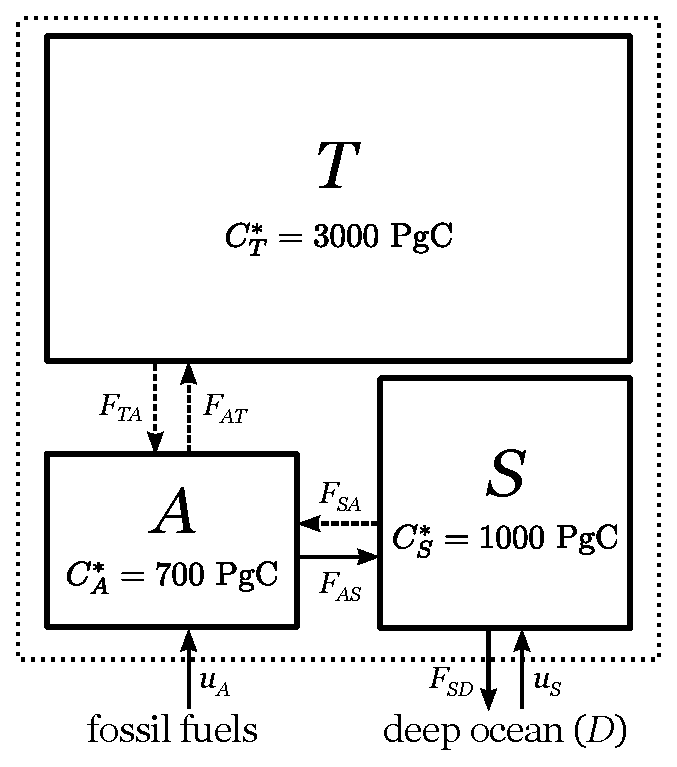
\includegraphics[height=0.9\textheight]{model2.pdf}
\end{frame}

%%%%%%%%%%%%%%%%%%%%%%%%%%%%%%%%%%%%%%%%%%%%%%%%%%%%%%%%%%%%%%%%%%%%%%%%%%%%%%%%%%%%%%%%%%%%%%%%%%%%%
\begin{frame}
	\frametitle{Hydrology Watersheds}
	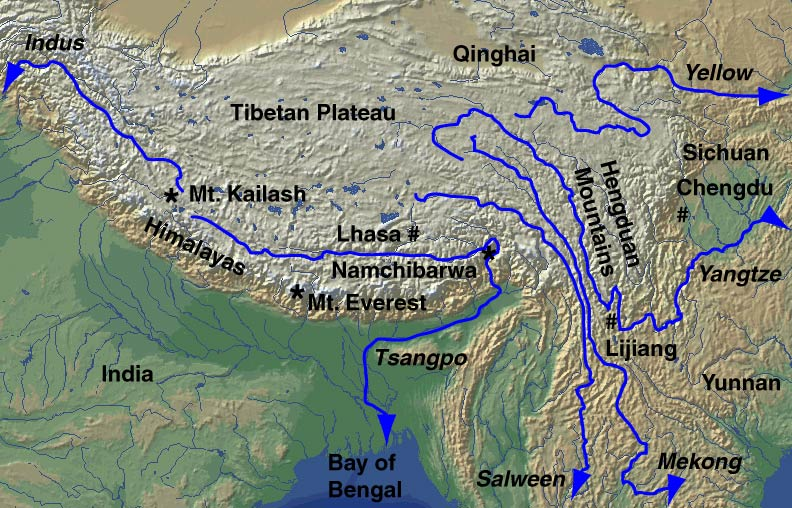
\includegraphics[width=0.9\textwidth]{Watersheds.jpeg}
\end{frame}
%%%%%%%%%%%%%%%%%%%%%%%%%%%%%%%%%%%%%%%%%%%%%%%%%%%%%%%%%%%%%%%%%%%%%%%%%%%%%%%%%%%%%%%%%%%%%%%%%%%%%
\begin{frame}
	\frametitle{Hydrology Catchments}
	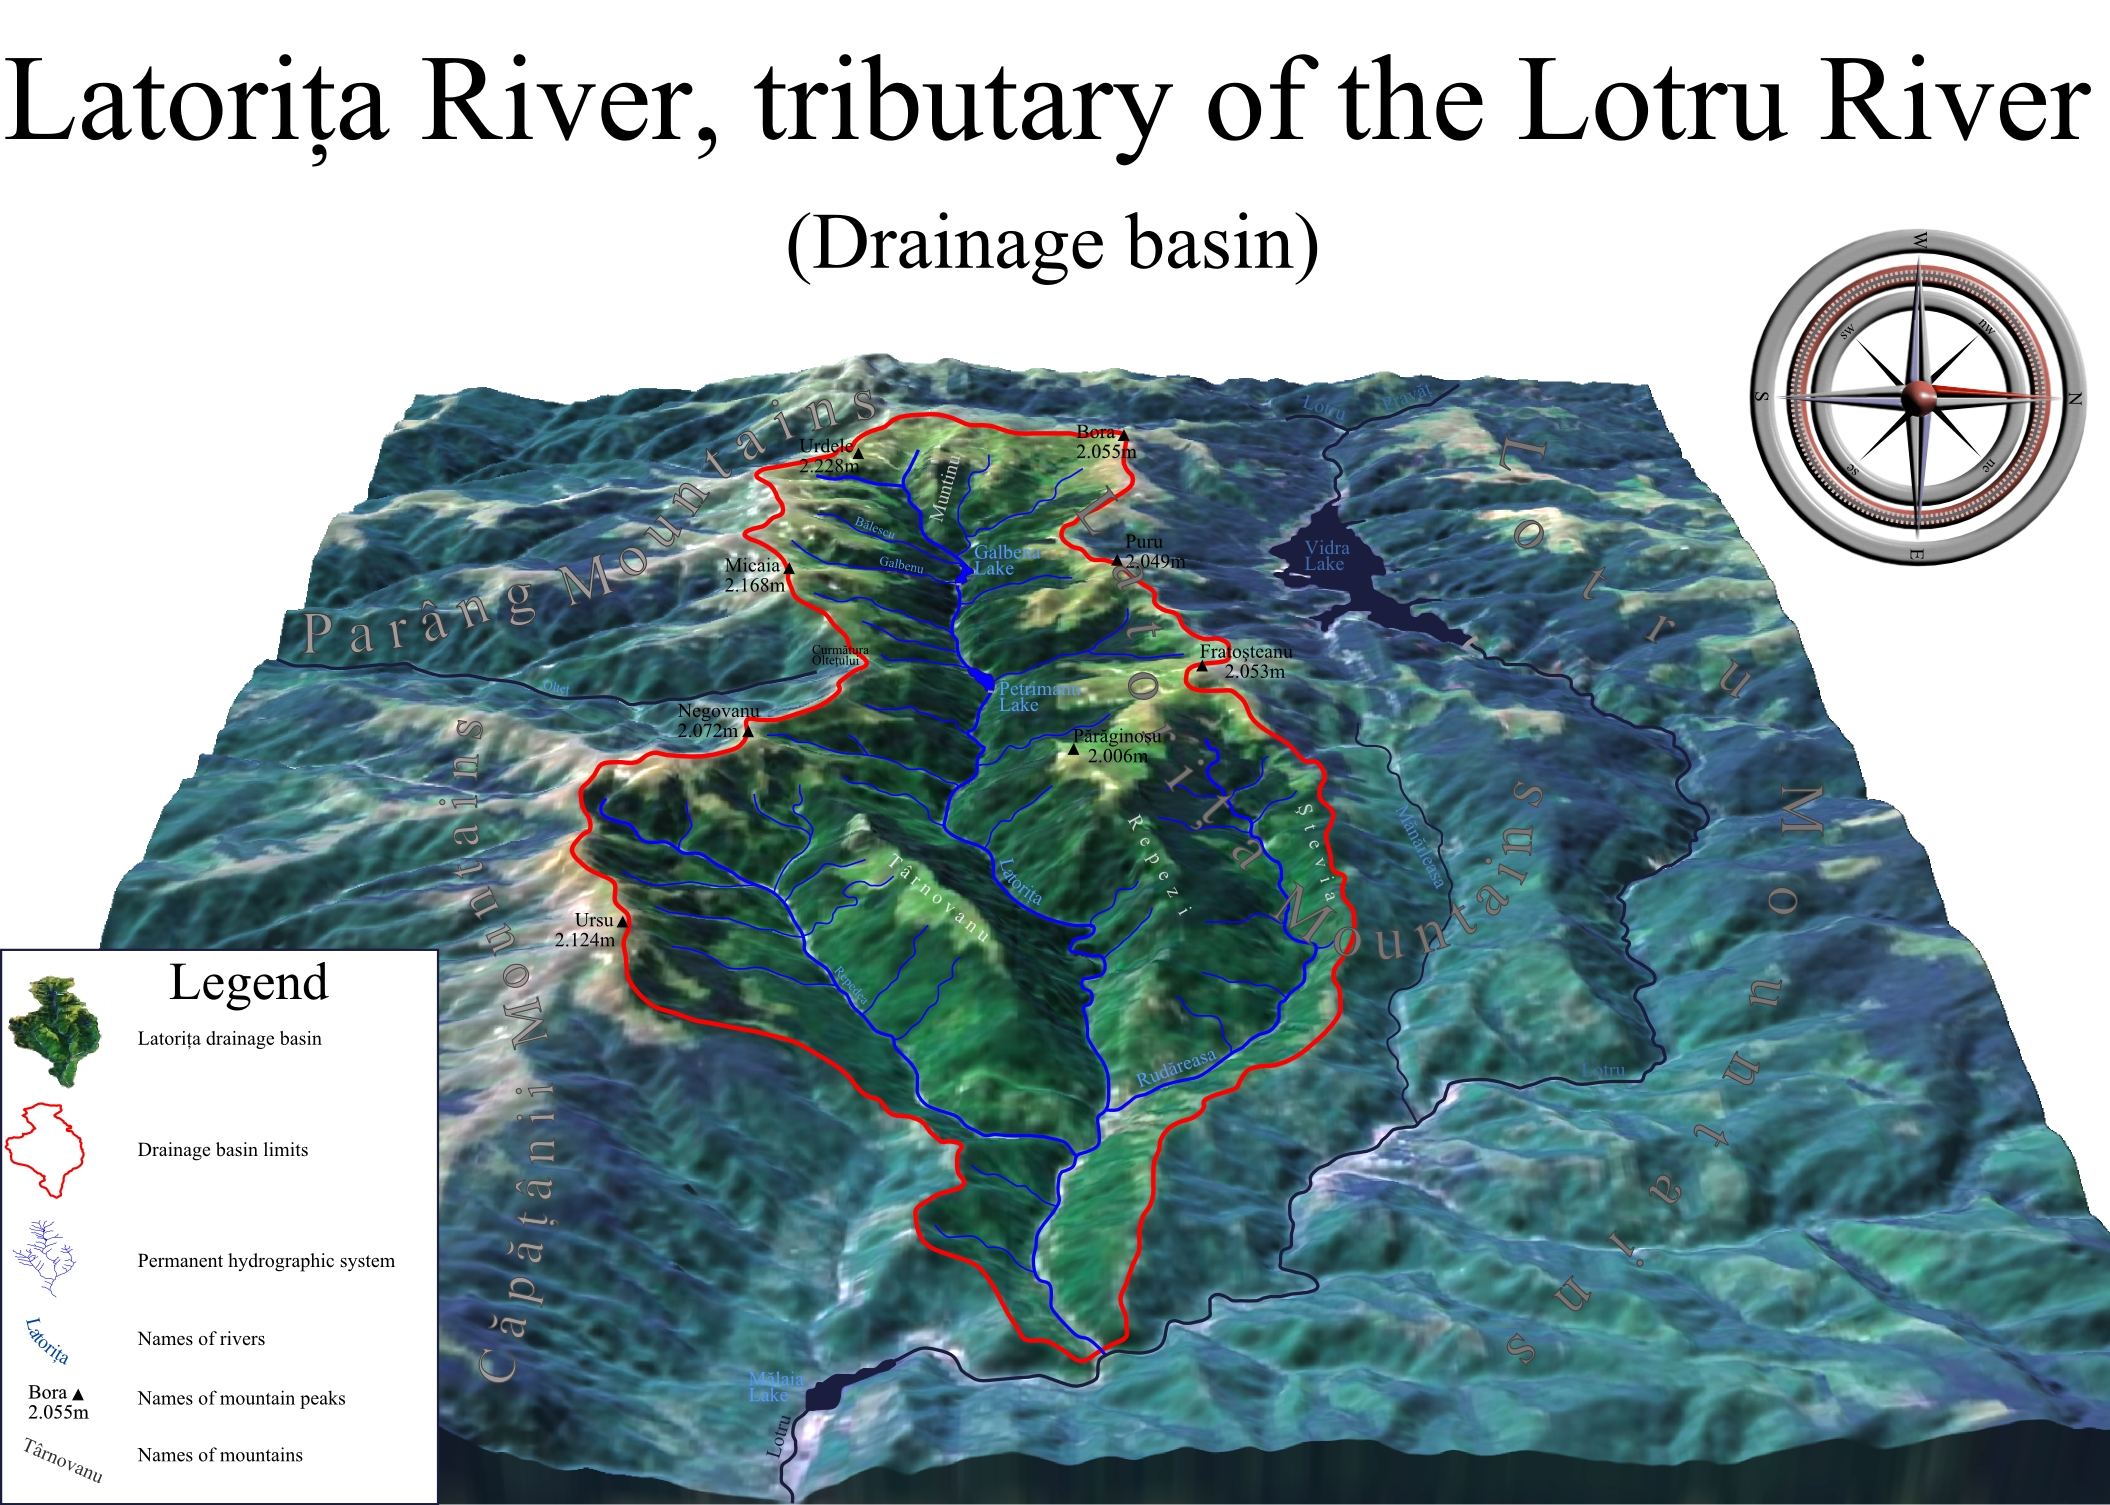
\includegraphics[width=0.9\textwidth]{EN_Bazinul_hidrografic_al_Raului_Latorita,_Romania.jpg}
\end{frame}
%%%%%%%%%%%%%%%%%%%%%%%%%%%%%%%%%%%%%%%%%%%%%%%%%%%%%%%%%%%%%%%%%%%%%%%%%%%%%%%%%%%%%%%%%%%%%%%%%%%%%
%%%%%%%%%%%%%%%%%%%%%%%%%%%%%%%%%%%%%%%%%%%%%%%%%%%%%%%%%%%%%%%%%%%%%%%%%%%%%%%%%%%%%%%%%%%%%%%%%%%%%
\begin{frame}
	\frametitle{Plant Physiology/ Carbon allocation}
	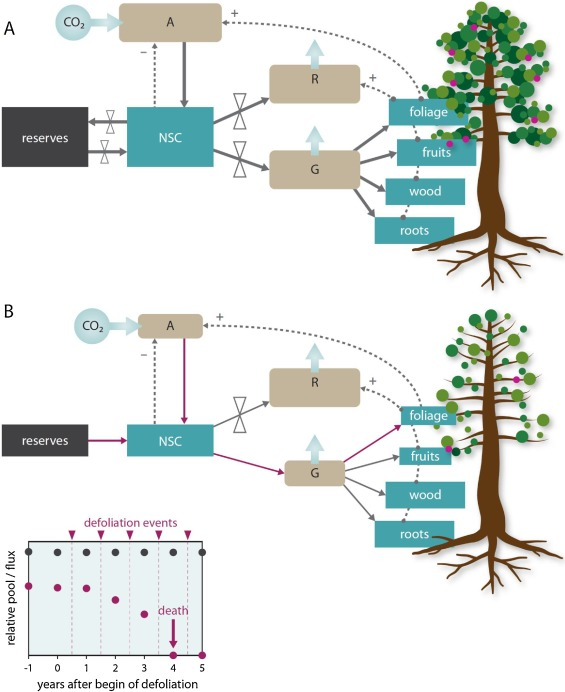
\includegraphics[height=0.9\textheight]{CarbonAllocation.jpg}
	\cite{Hartmann2018EEB}
\end{frame}
%%%%%%%%%%%%%%%%%%%%%%%%%%%%%%%%%%%%%%%%%%%%%%%%%%%%%%%%%%%%%%%%%%%%%%%%%%%%%%%%%%%%%%%%%%%%%%%%%%%%%
\begin{frame}
	\frametitle{Organic Matter Decomposition / Soil Models}
	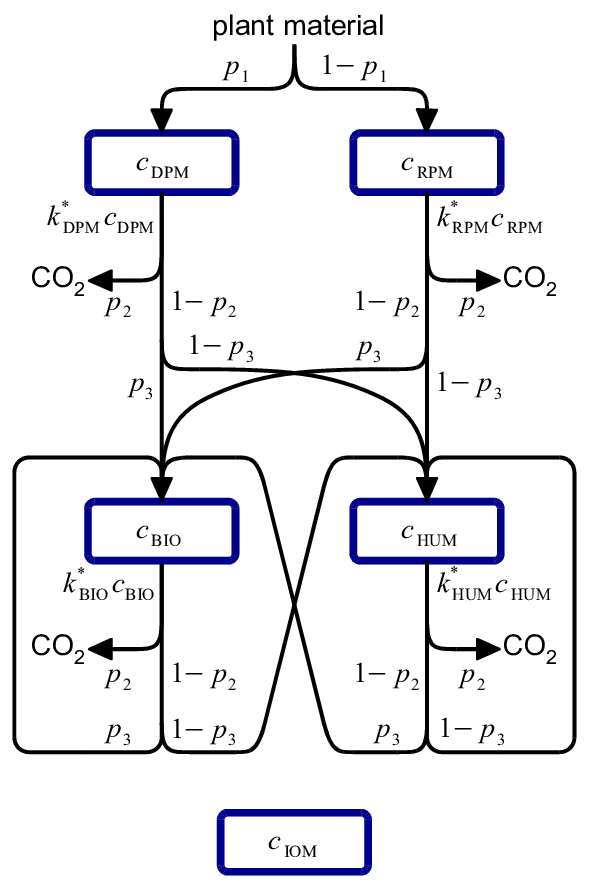
\includegraphics[width=0.35\textwidth]{RothC.png}
	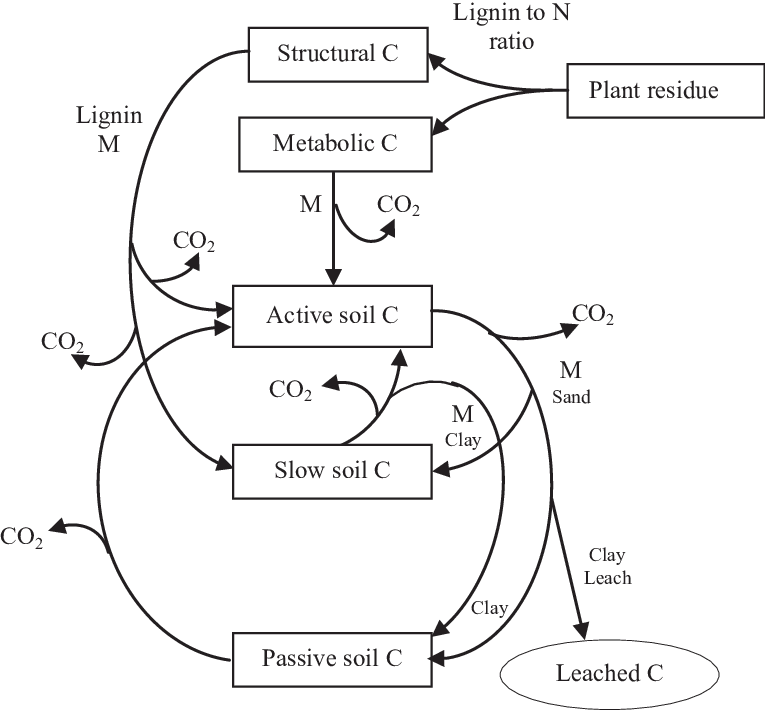
\includegraphics[width=0.55\textwidth]{Century.png}
\end{frame}
%%%%%%%%%%%%%%%%%%%%%%%%%%%%%%%%%%%%%%%%%%%%%%%%%%%%%%%%%%%%%%%%%%%%%%%%%%%%%%%%%%%%%%%%%%%%%%%%%%%%%
\begin{frame}
	\frametitle{Ecosystem Models}
	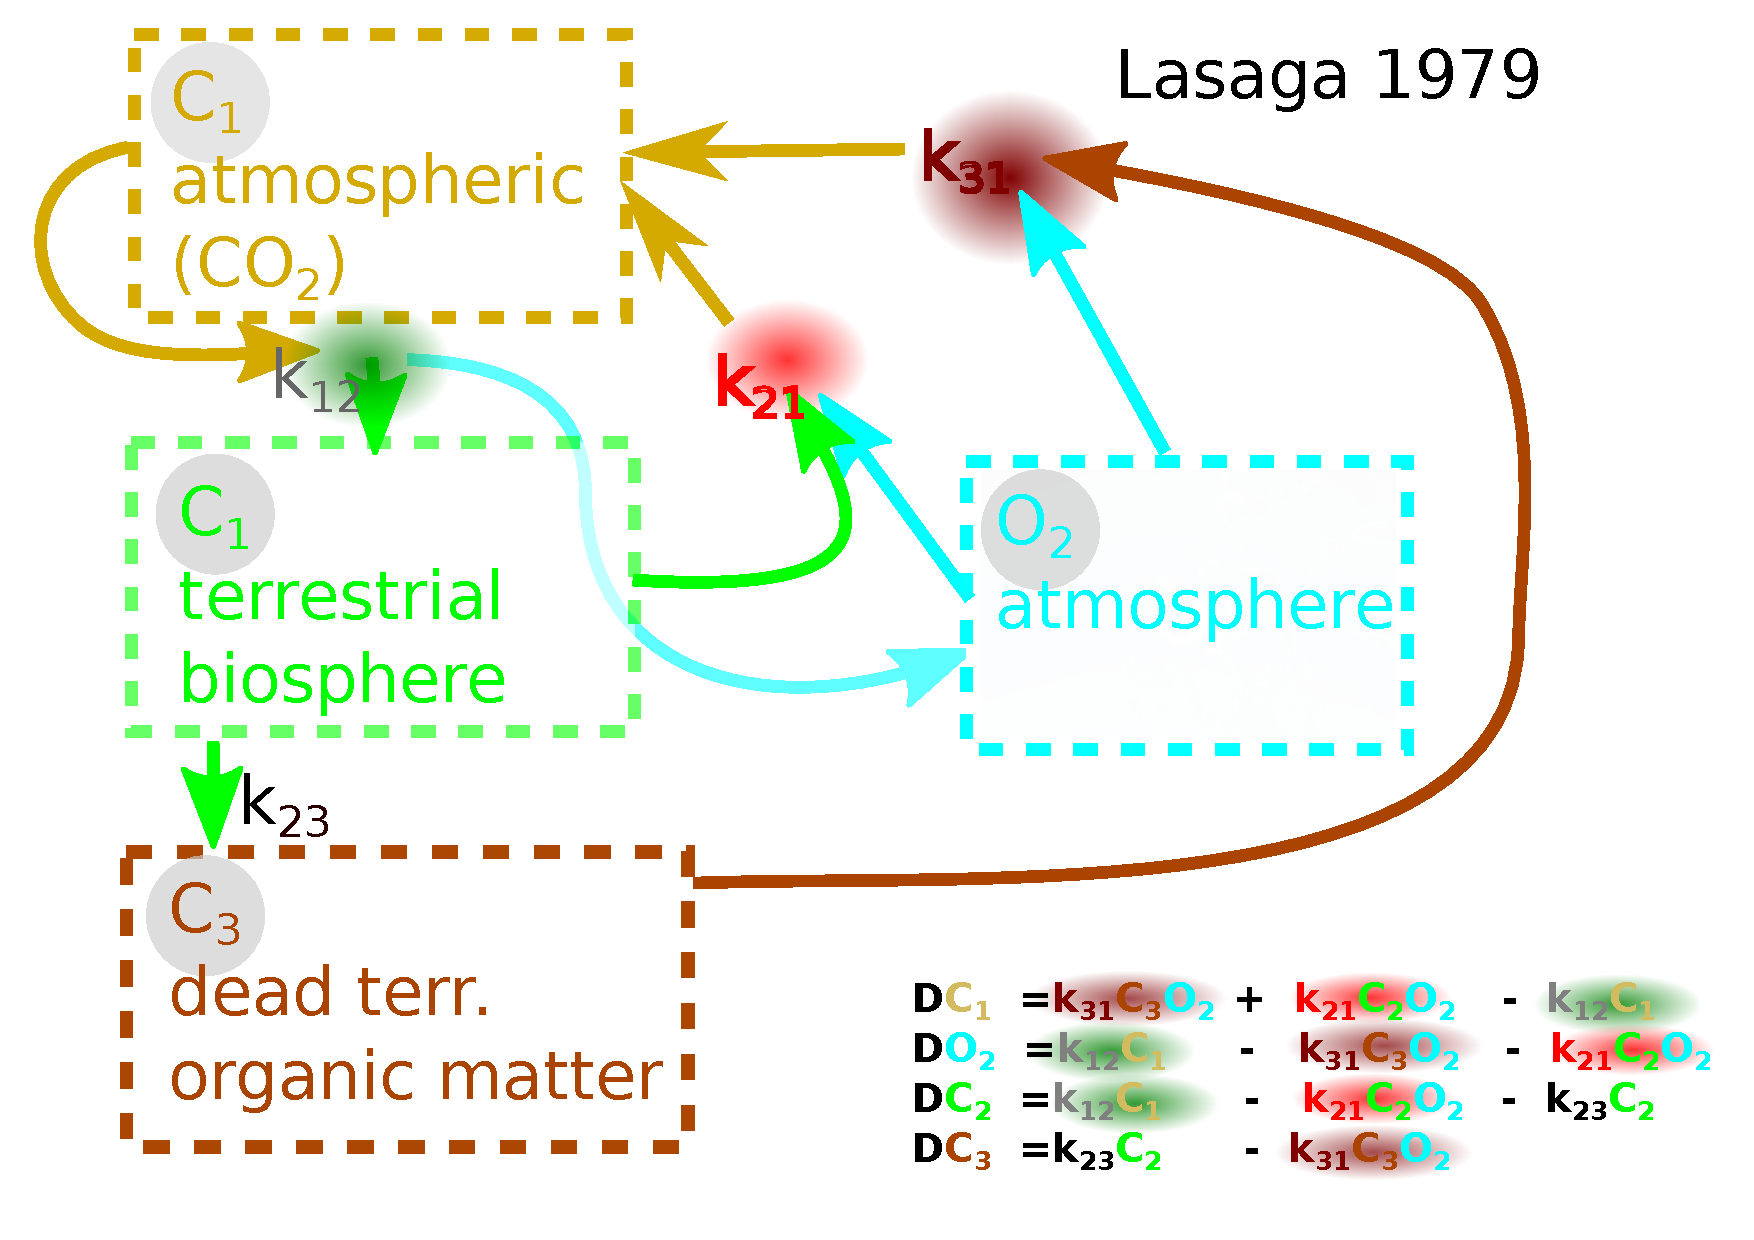
\includegraphics[width=0.9\textwidth]{LasagaModel.pdf}
\end{frame}
%%%%%%%%%%%%%%%%%%%%%%%%%%%%%%%%%%%%%%%%%%%%%%%%%%%%%%%%%%%%%%%%%%%%%%%%%%%%%%%%%%%%%%%%%%%%%%%%%%%%%
\begin{frame}
	\frametitle{Chemical Reactors}
	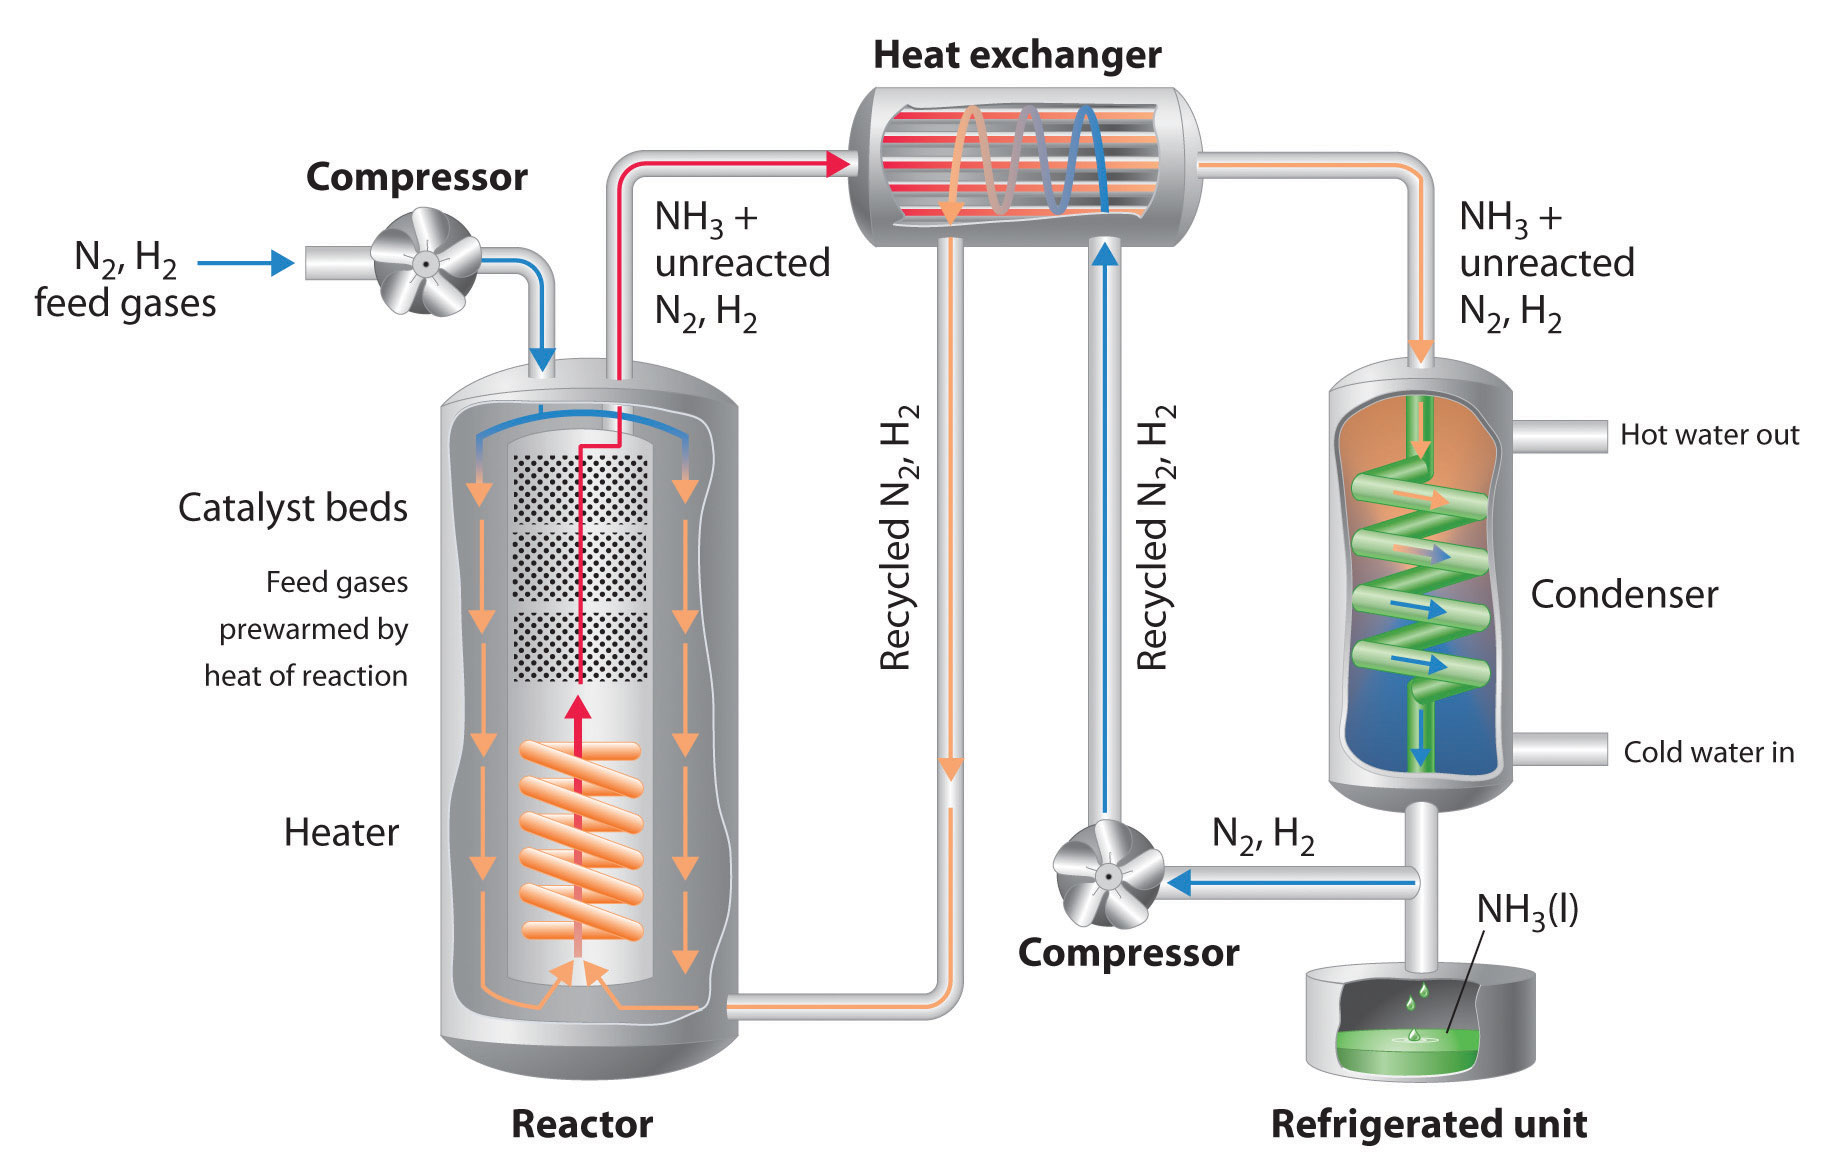
\includegraphics[width=0.9\textwidth]{HaberBosch.jpg}
\end{frame}
%%%%%%%%%%%%%%%%%%%%%%%%%%%%%%%%%%%%%%%%%%%%%%%%%%%%%%%%%%%%%%%%%%%%%%%%%%%%%%%%%%%%%%%%%%%%%%%%%%%%%
\begin{frame}
	\frametitle{Population Dynamics}
	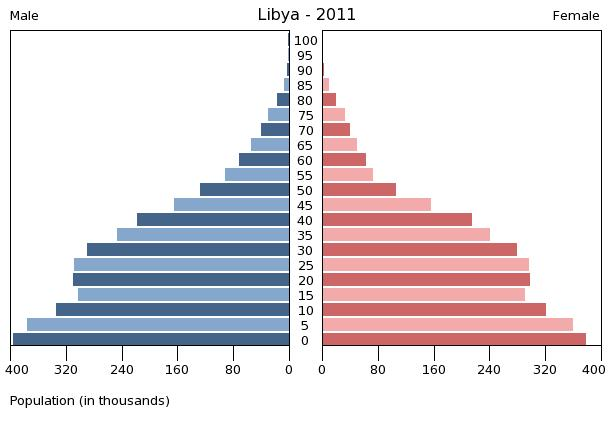
\includegraphics[width=0.9\textwidth]{LibyaPopulation2011.jpg}
\end{frame}
%%%%%%%%%%%%%%%%%%%%%%%%%%%%%%%%%%%%%%%%%%%%%%%%%%%%%%%%%%%%%%%%%%%%%%%%%%%%%%%%%%%%%%%%%%%%%%%%%%%%%
\section{Reducing Model Complexity }
\subsection{The Carbon Cycle example}
%%%%%%%%%%%%%%%%%%%%%%%%%%%%%%%%%%%%%%%%%%%%%%%%%%%%%%%%%%%%%%%%%%%%%%%%%%%%%%%%%%%%%%%%%%%%%%%%%%%%
%%%%%%%%%%%%%%%%%%%%%%%%%%%%%%%%%%%%%%%%%%%%%%%%%%%%%%%%%%%%%%%%%%%%%%%%%%%%%%%%%%%%%%%%%%%%%%%%%%%%%
\begin{frame}
  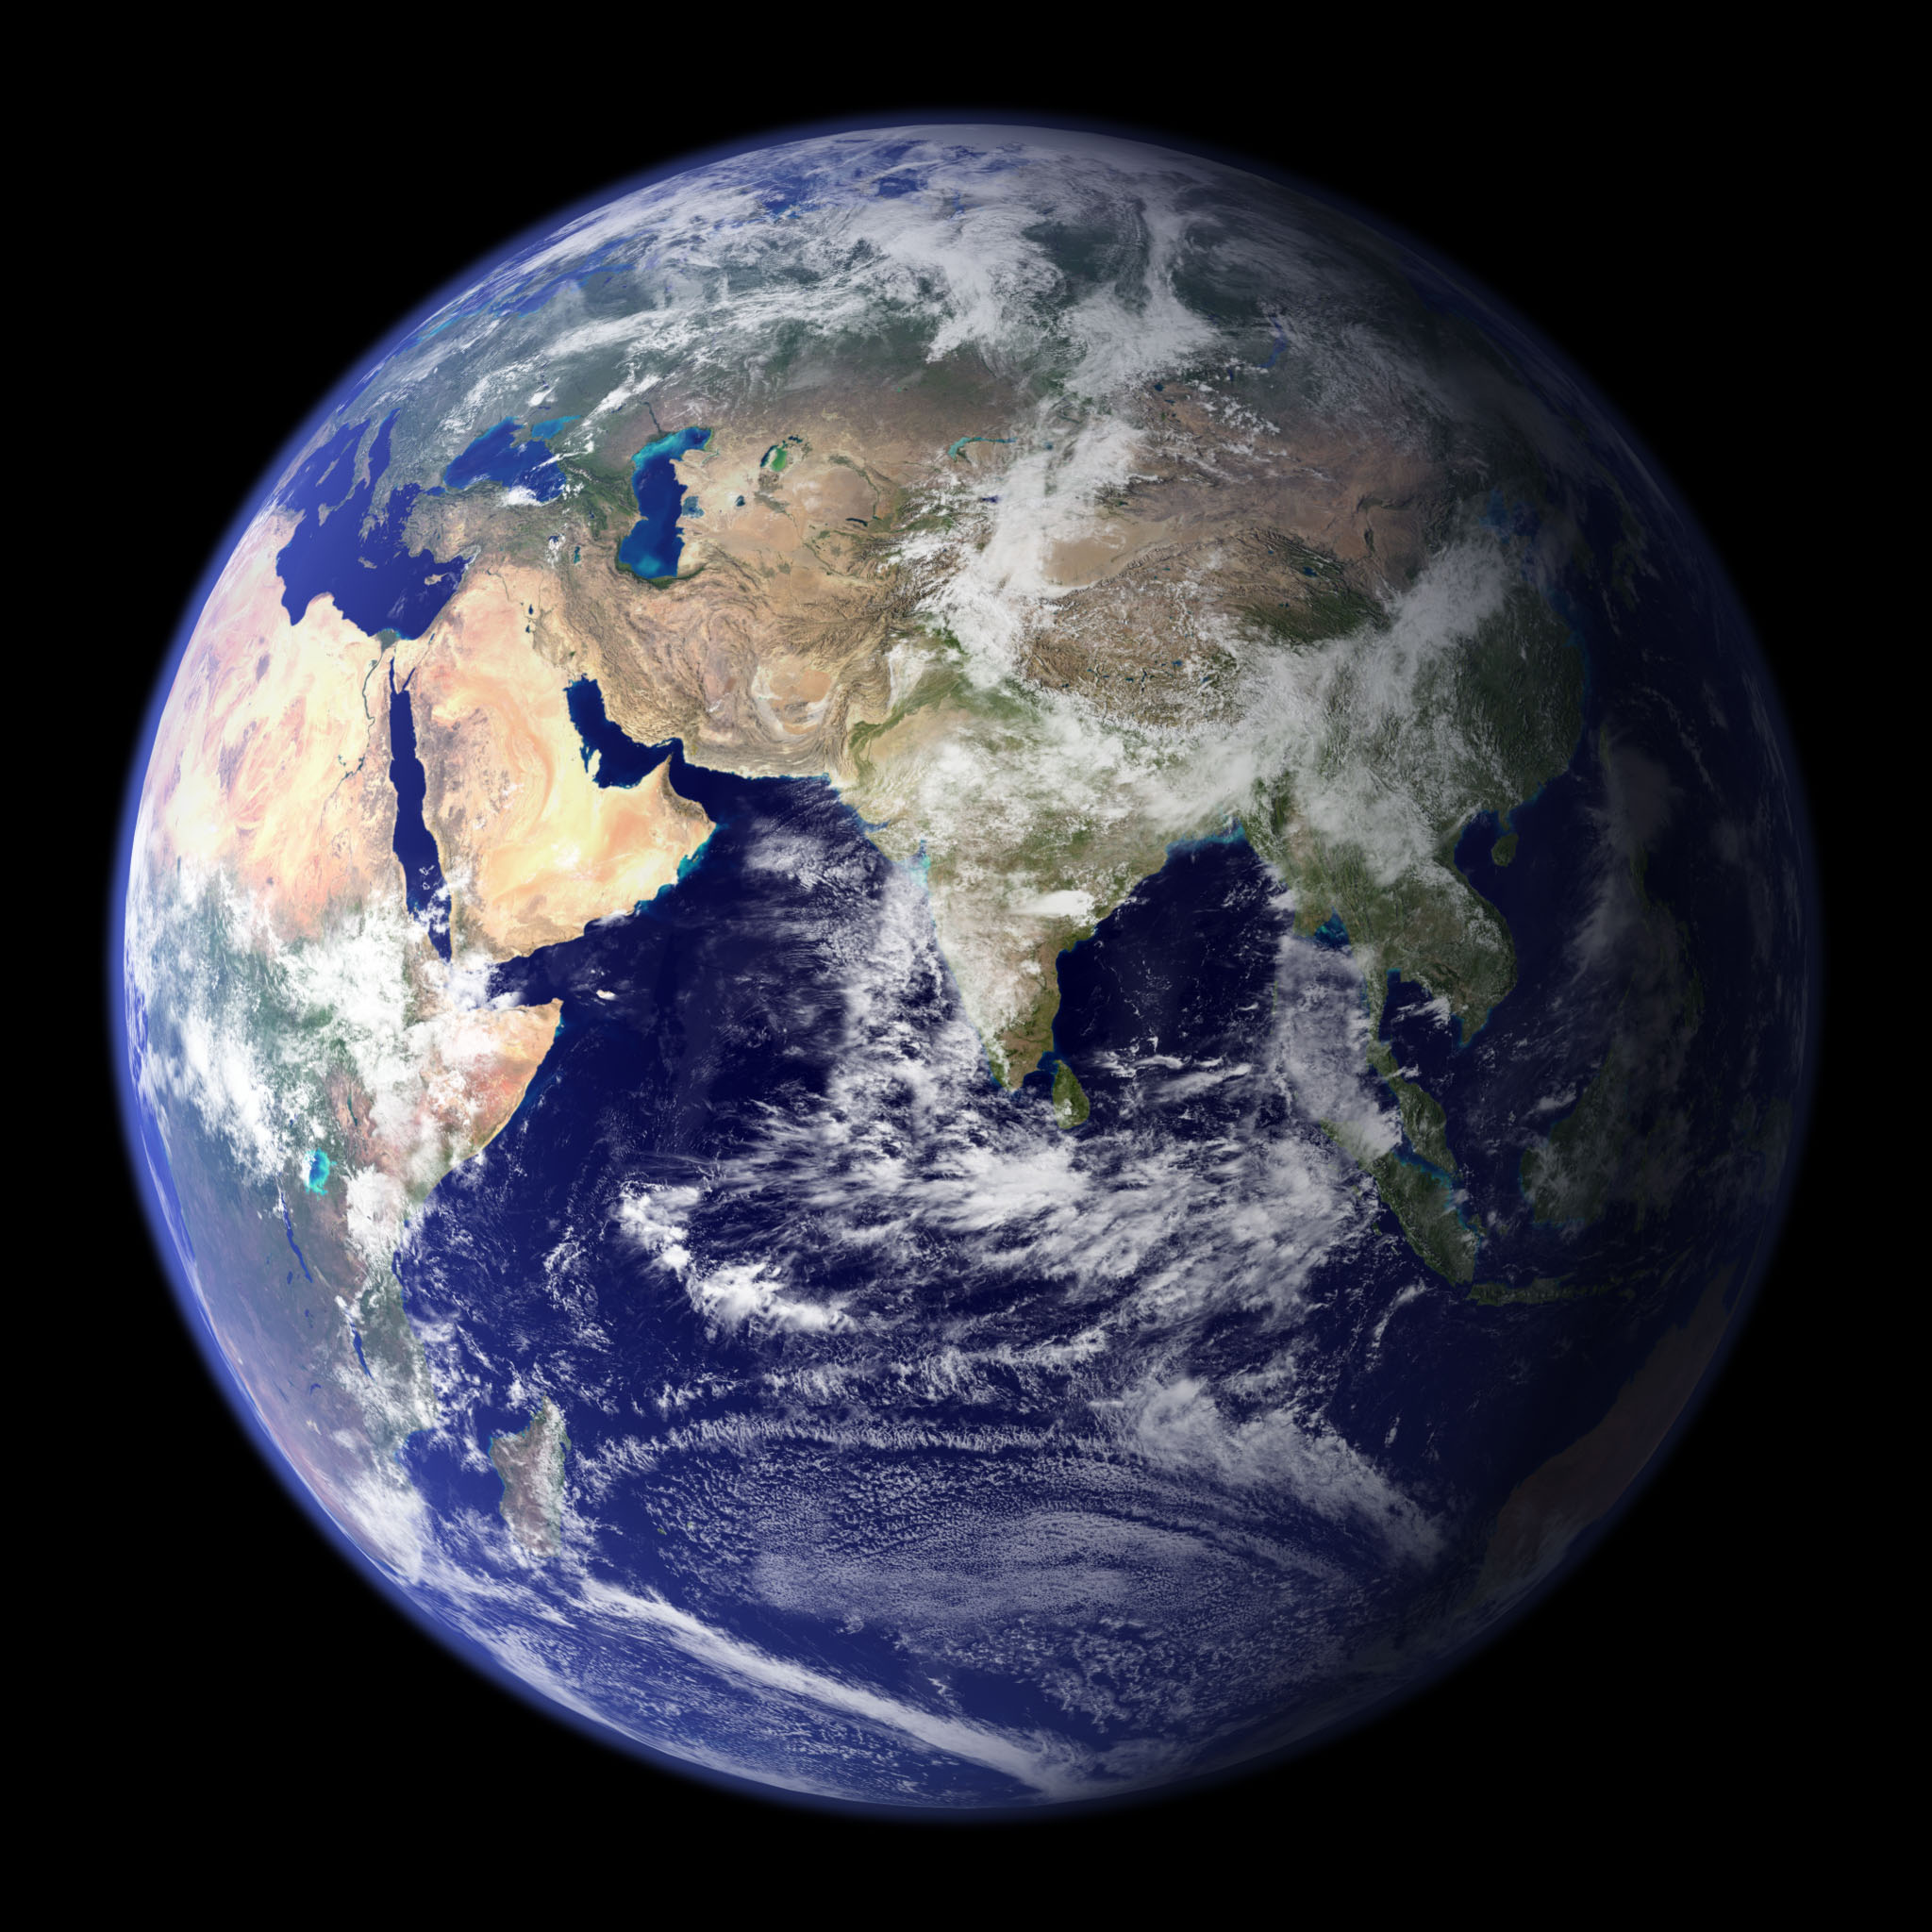
\includegraphics[width=0.3\textwidth]{Earth.jpg}
\end{frame}
%%%%%%%%%%%%%%%%%%%%%%%%%%%%%%%%%%%%%%%%%%%%%%%%%%%%%%%%%%%%%%%%%%%%%%%%%%%%%%%%%%%%%%%%%%%%%%%%%%%%%
\begin{frame}
  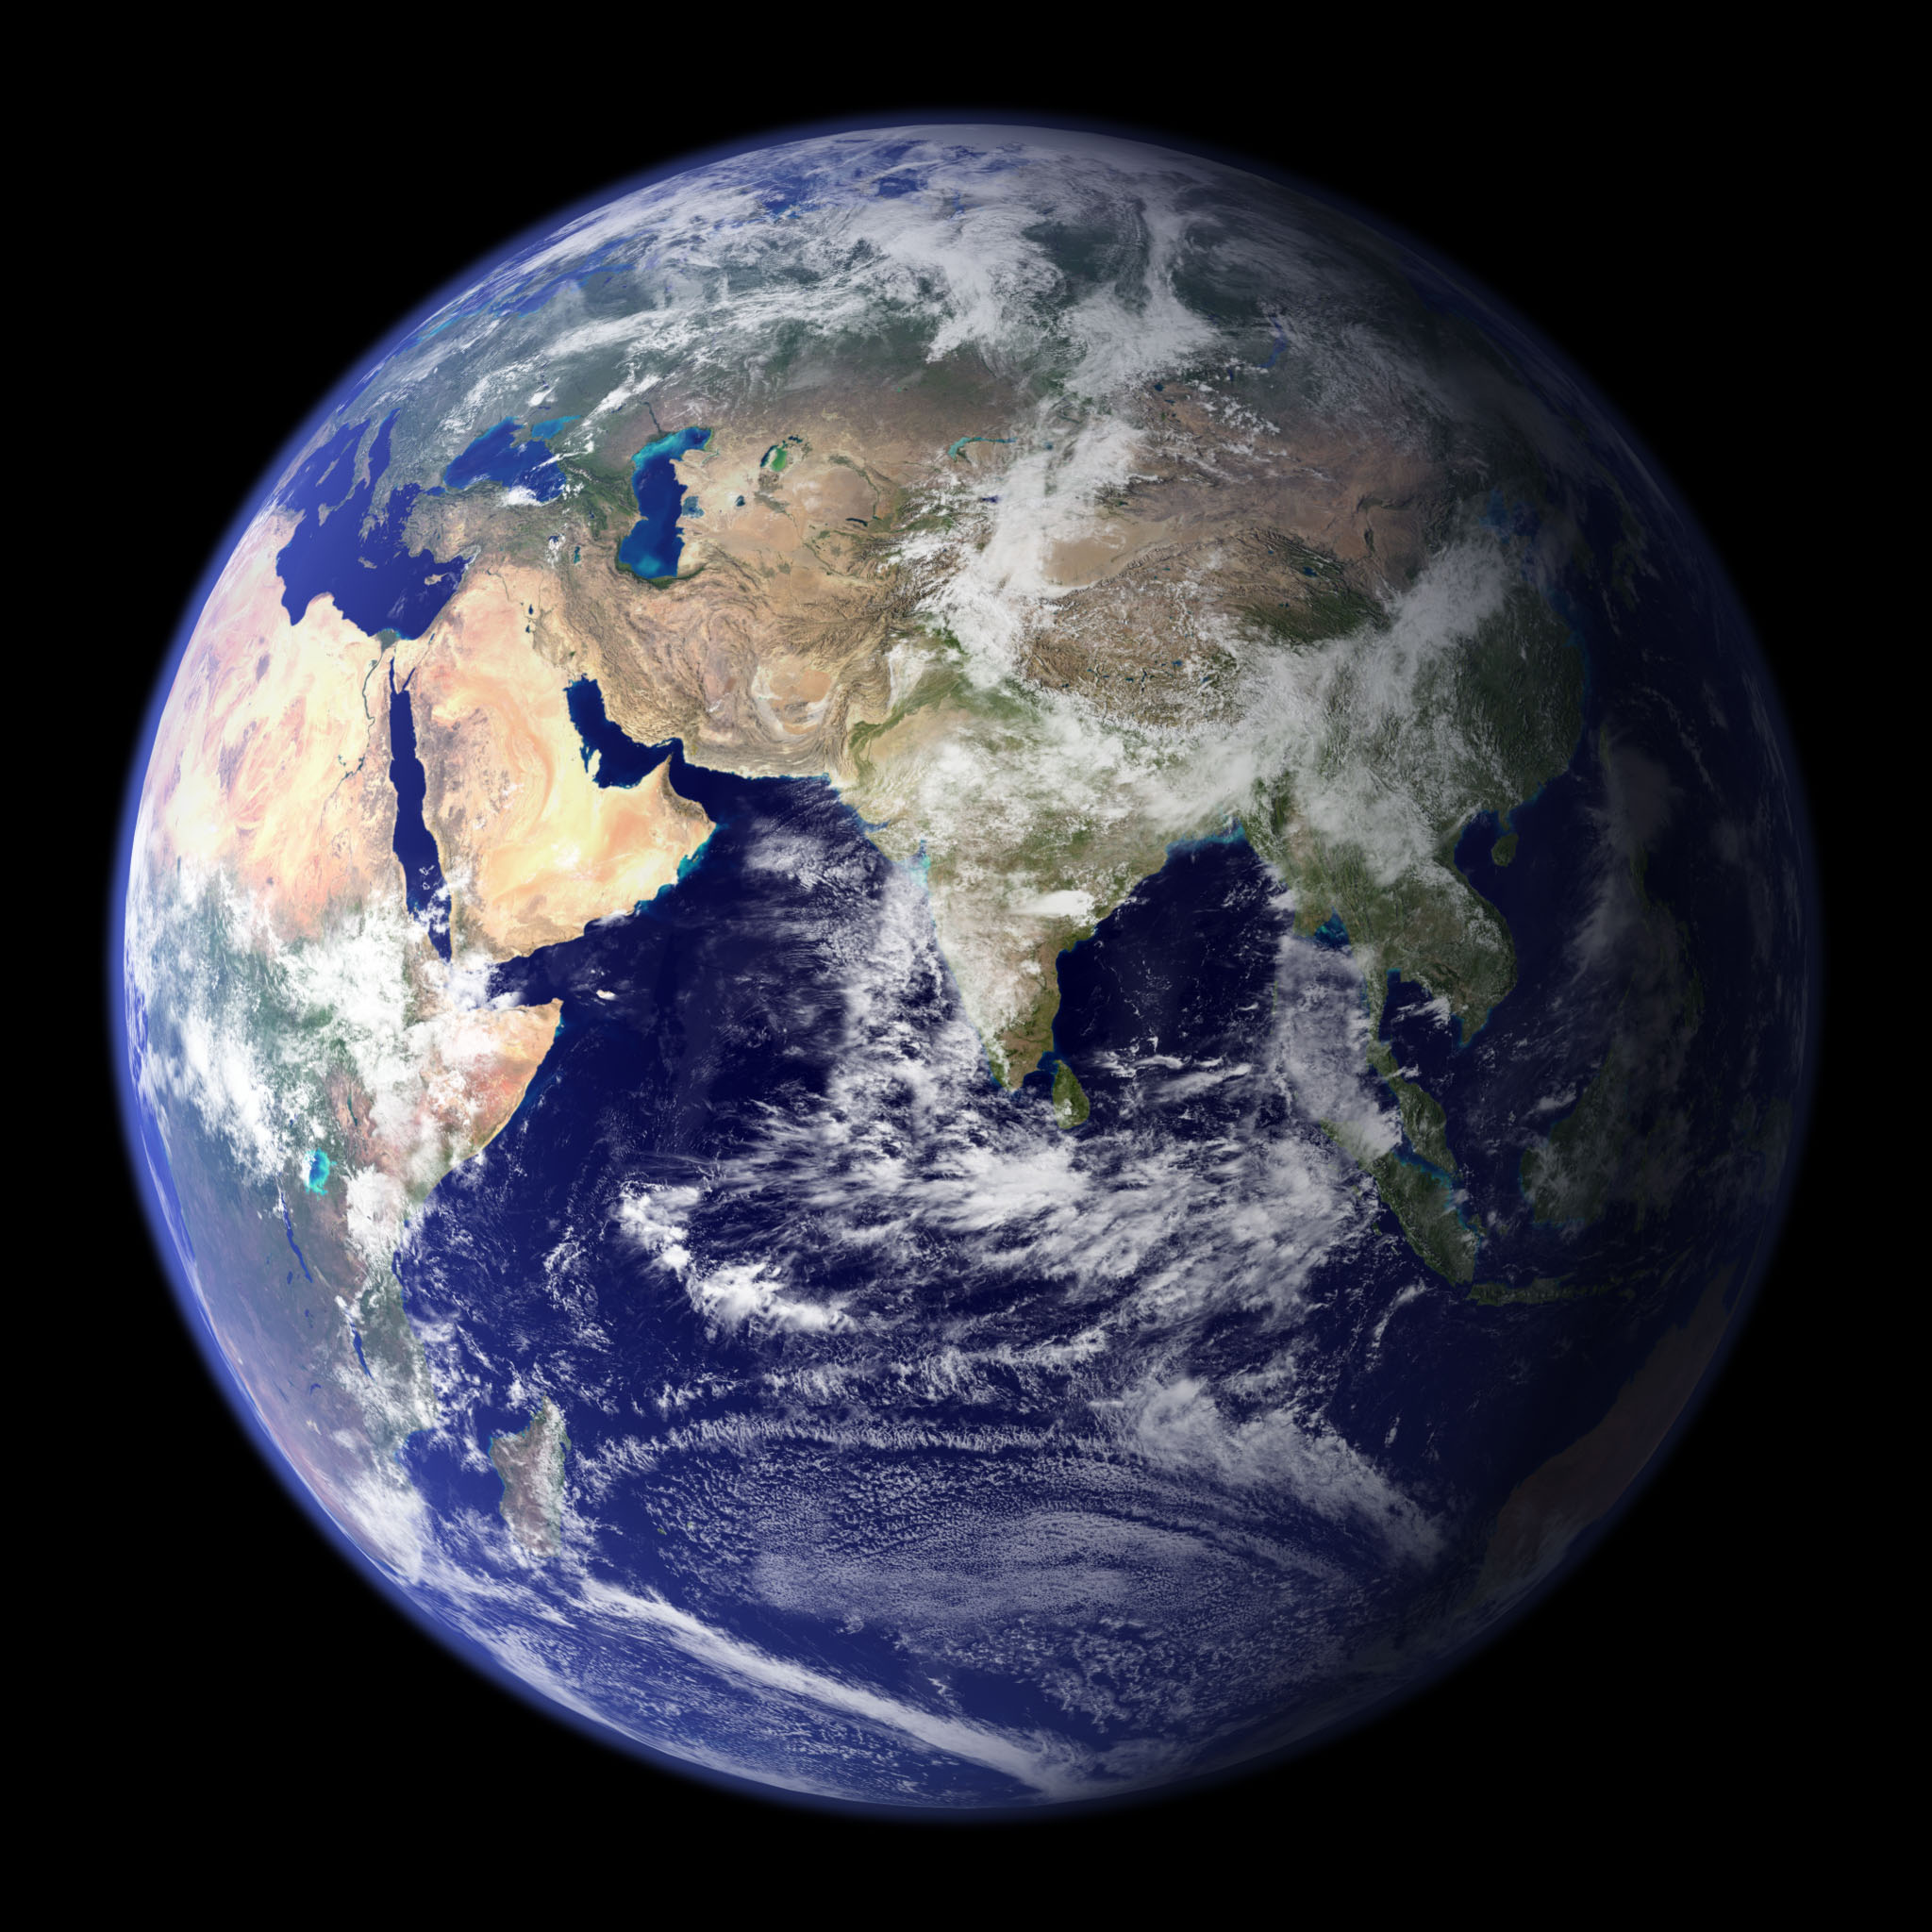
\includegraphics[width=0.3\textwidth]{Earth.jpg}
\end{frame}
%%%%%%%%%%%%%%%%%%%%%%%%%%%%%%%%%%%%%%%%%%%%%%%%%%%%%%%%%%%%%%%%%%%%%%%%%%%%%%%%%%%%%%%%%%%%%%%%%%%%%
\begin{frame}
  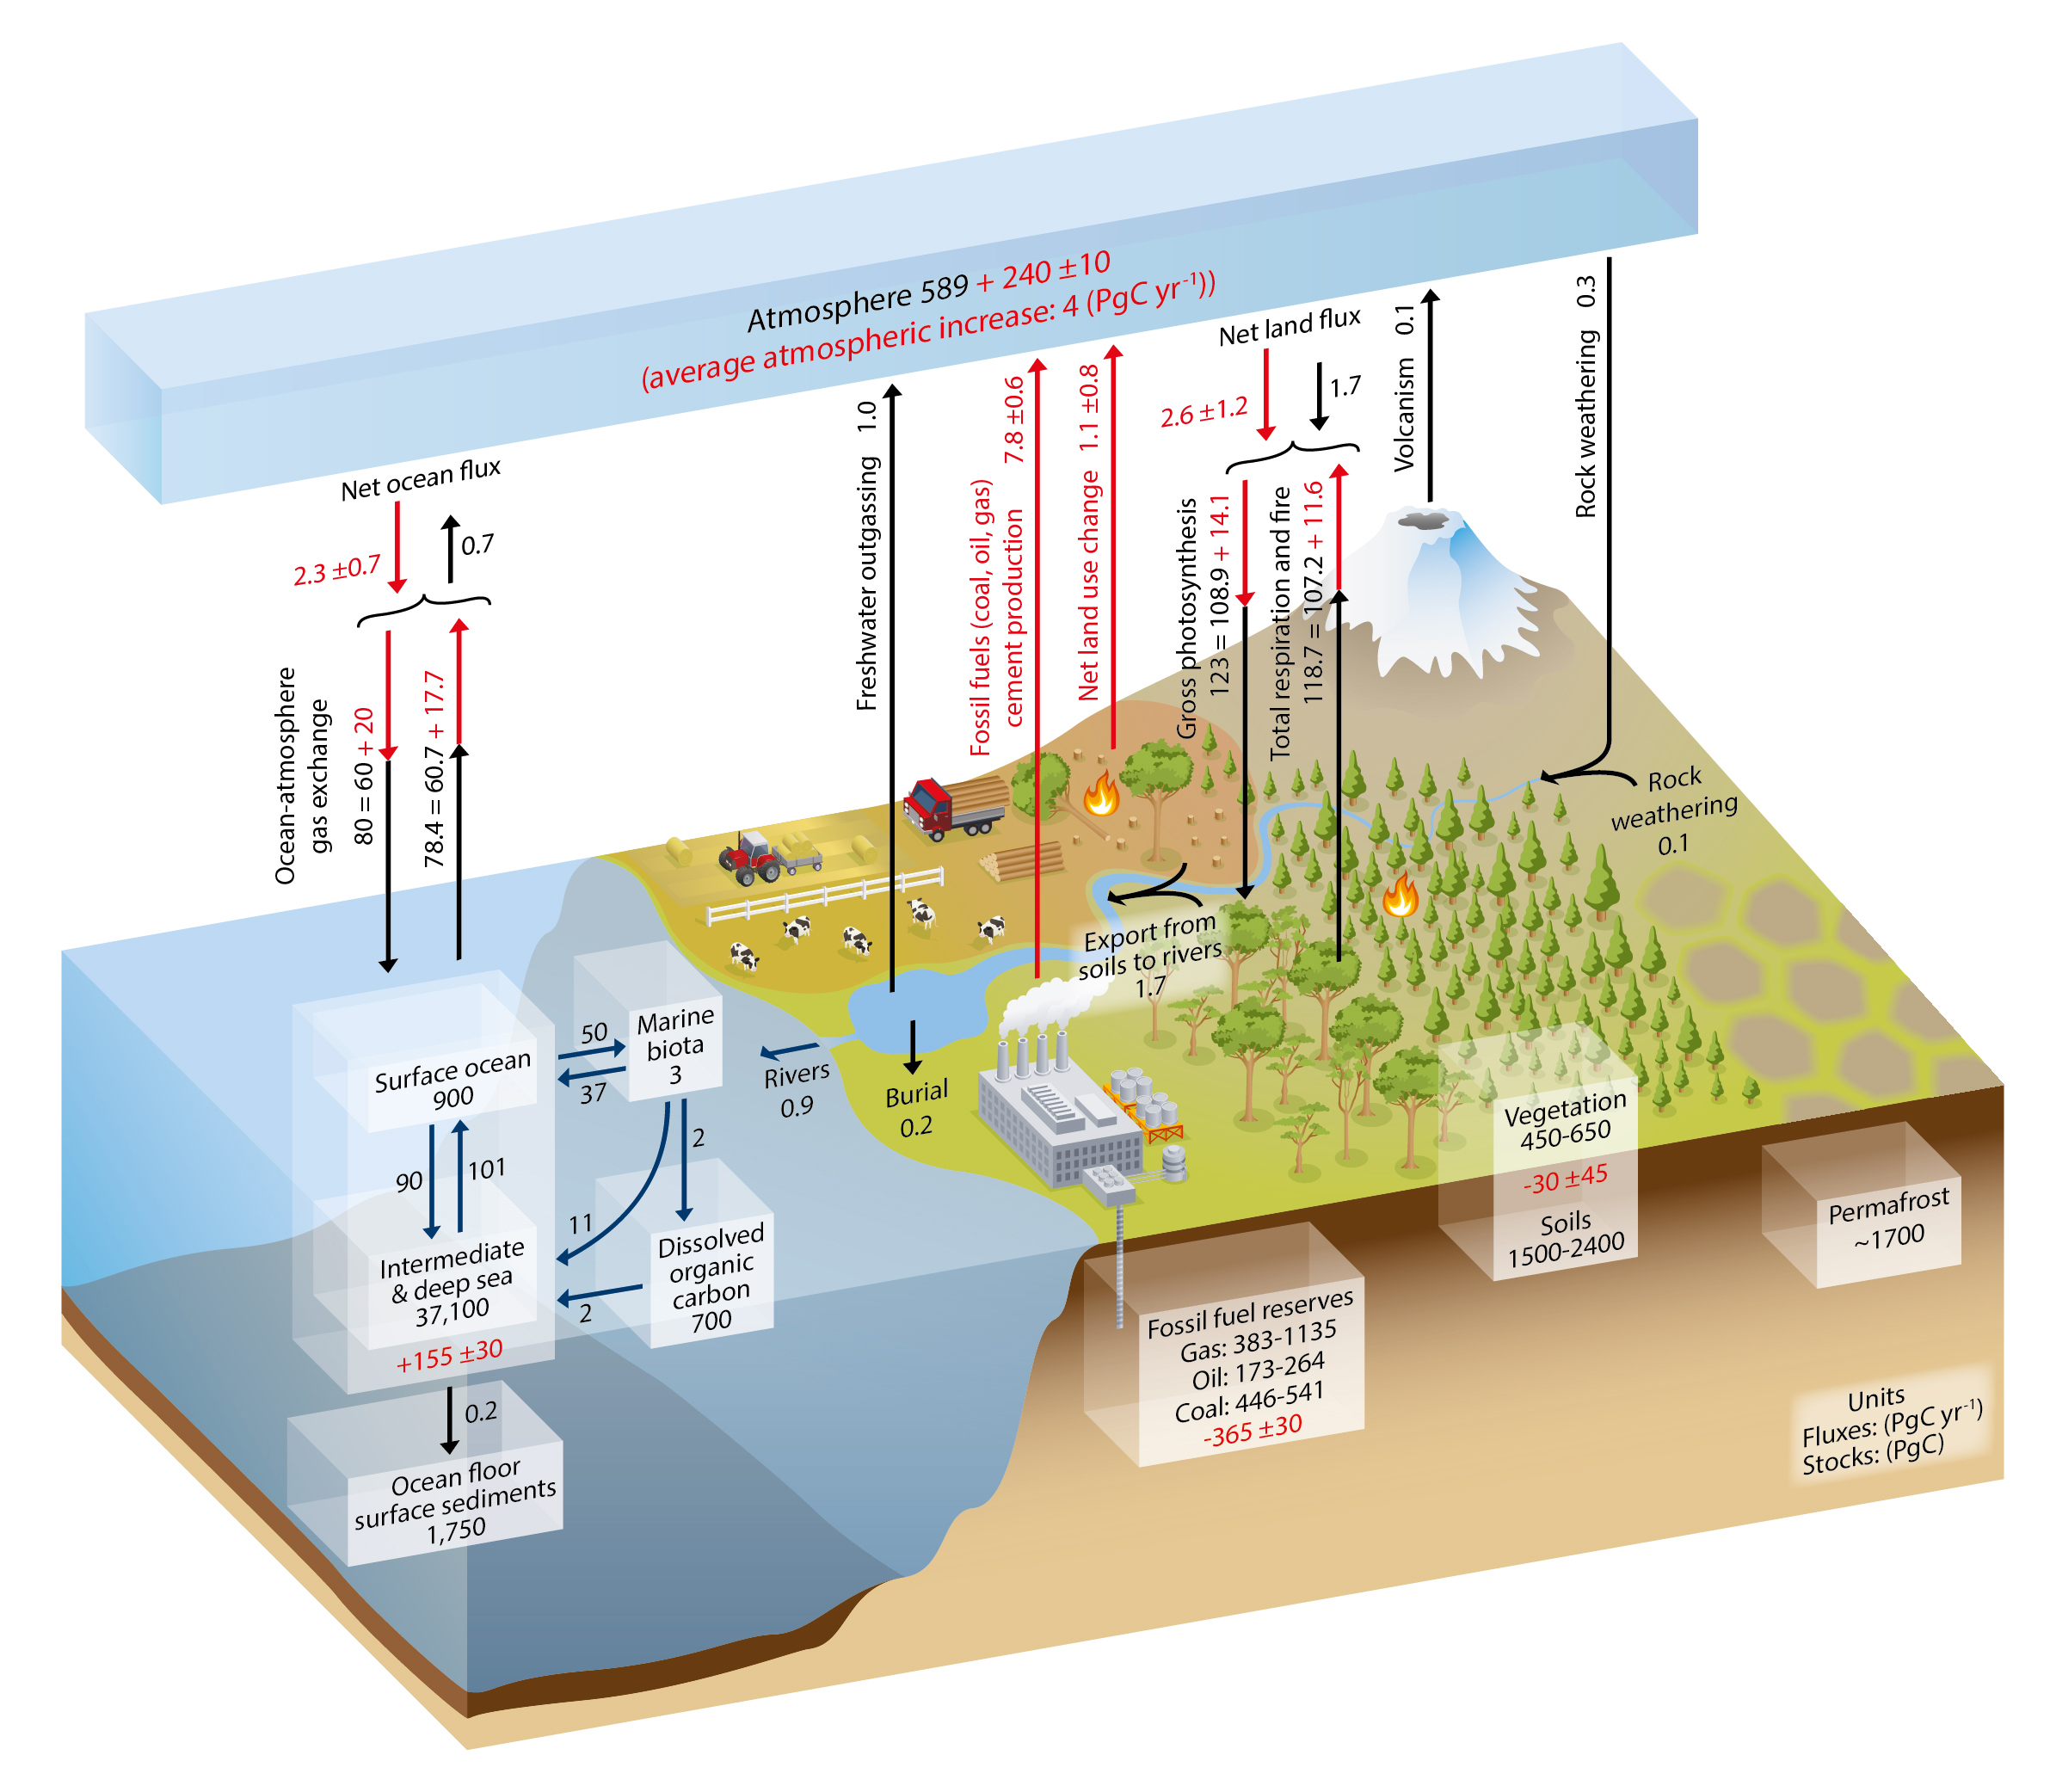
\includegraphics[width=0.9\textwidth]{cCycleIPCC.jpg}
\end{frame}
%%%%%%%%%%%%%%%%%%%%%%%%%%%%%%%%%%%%%%%%%%%%%%%%%%%%%%%%%%%%%%%%%%%%%%%%%%%%%%%%%%%%%%%%%%%%%%%%%%%%%
\begin{frame}
  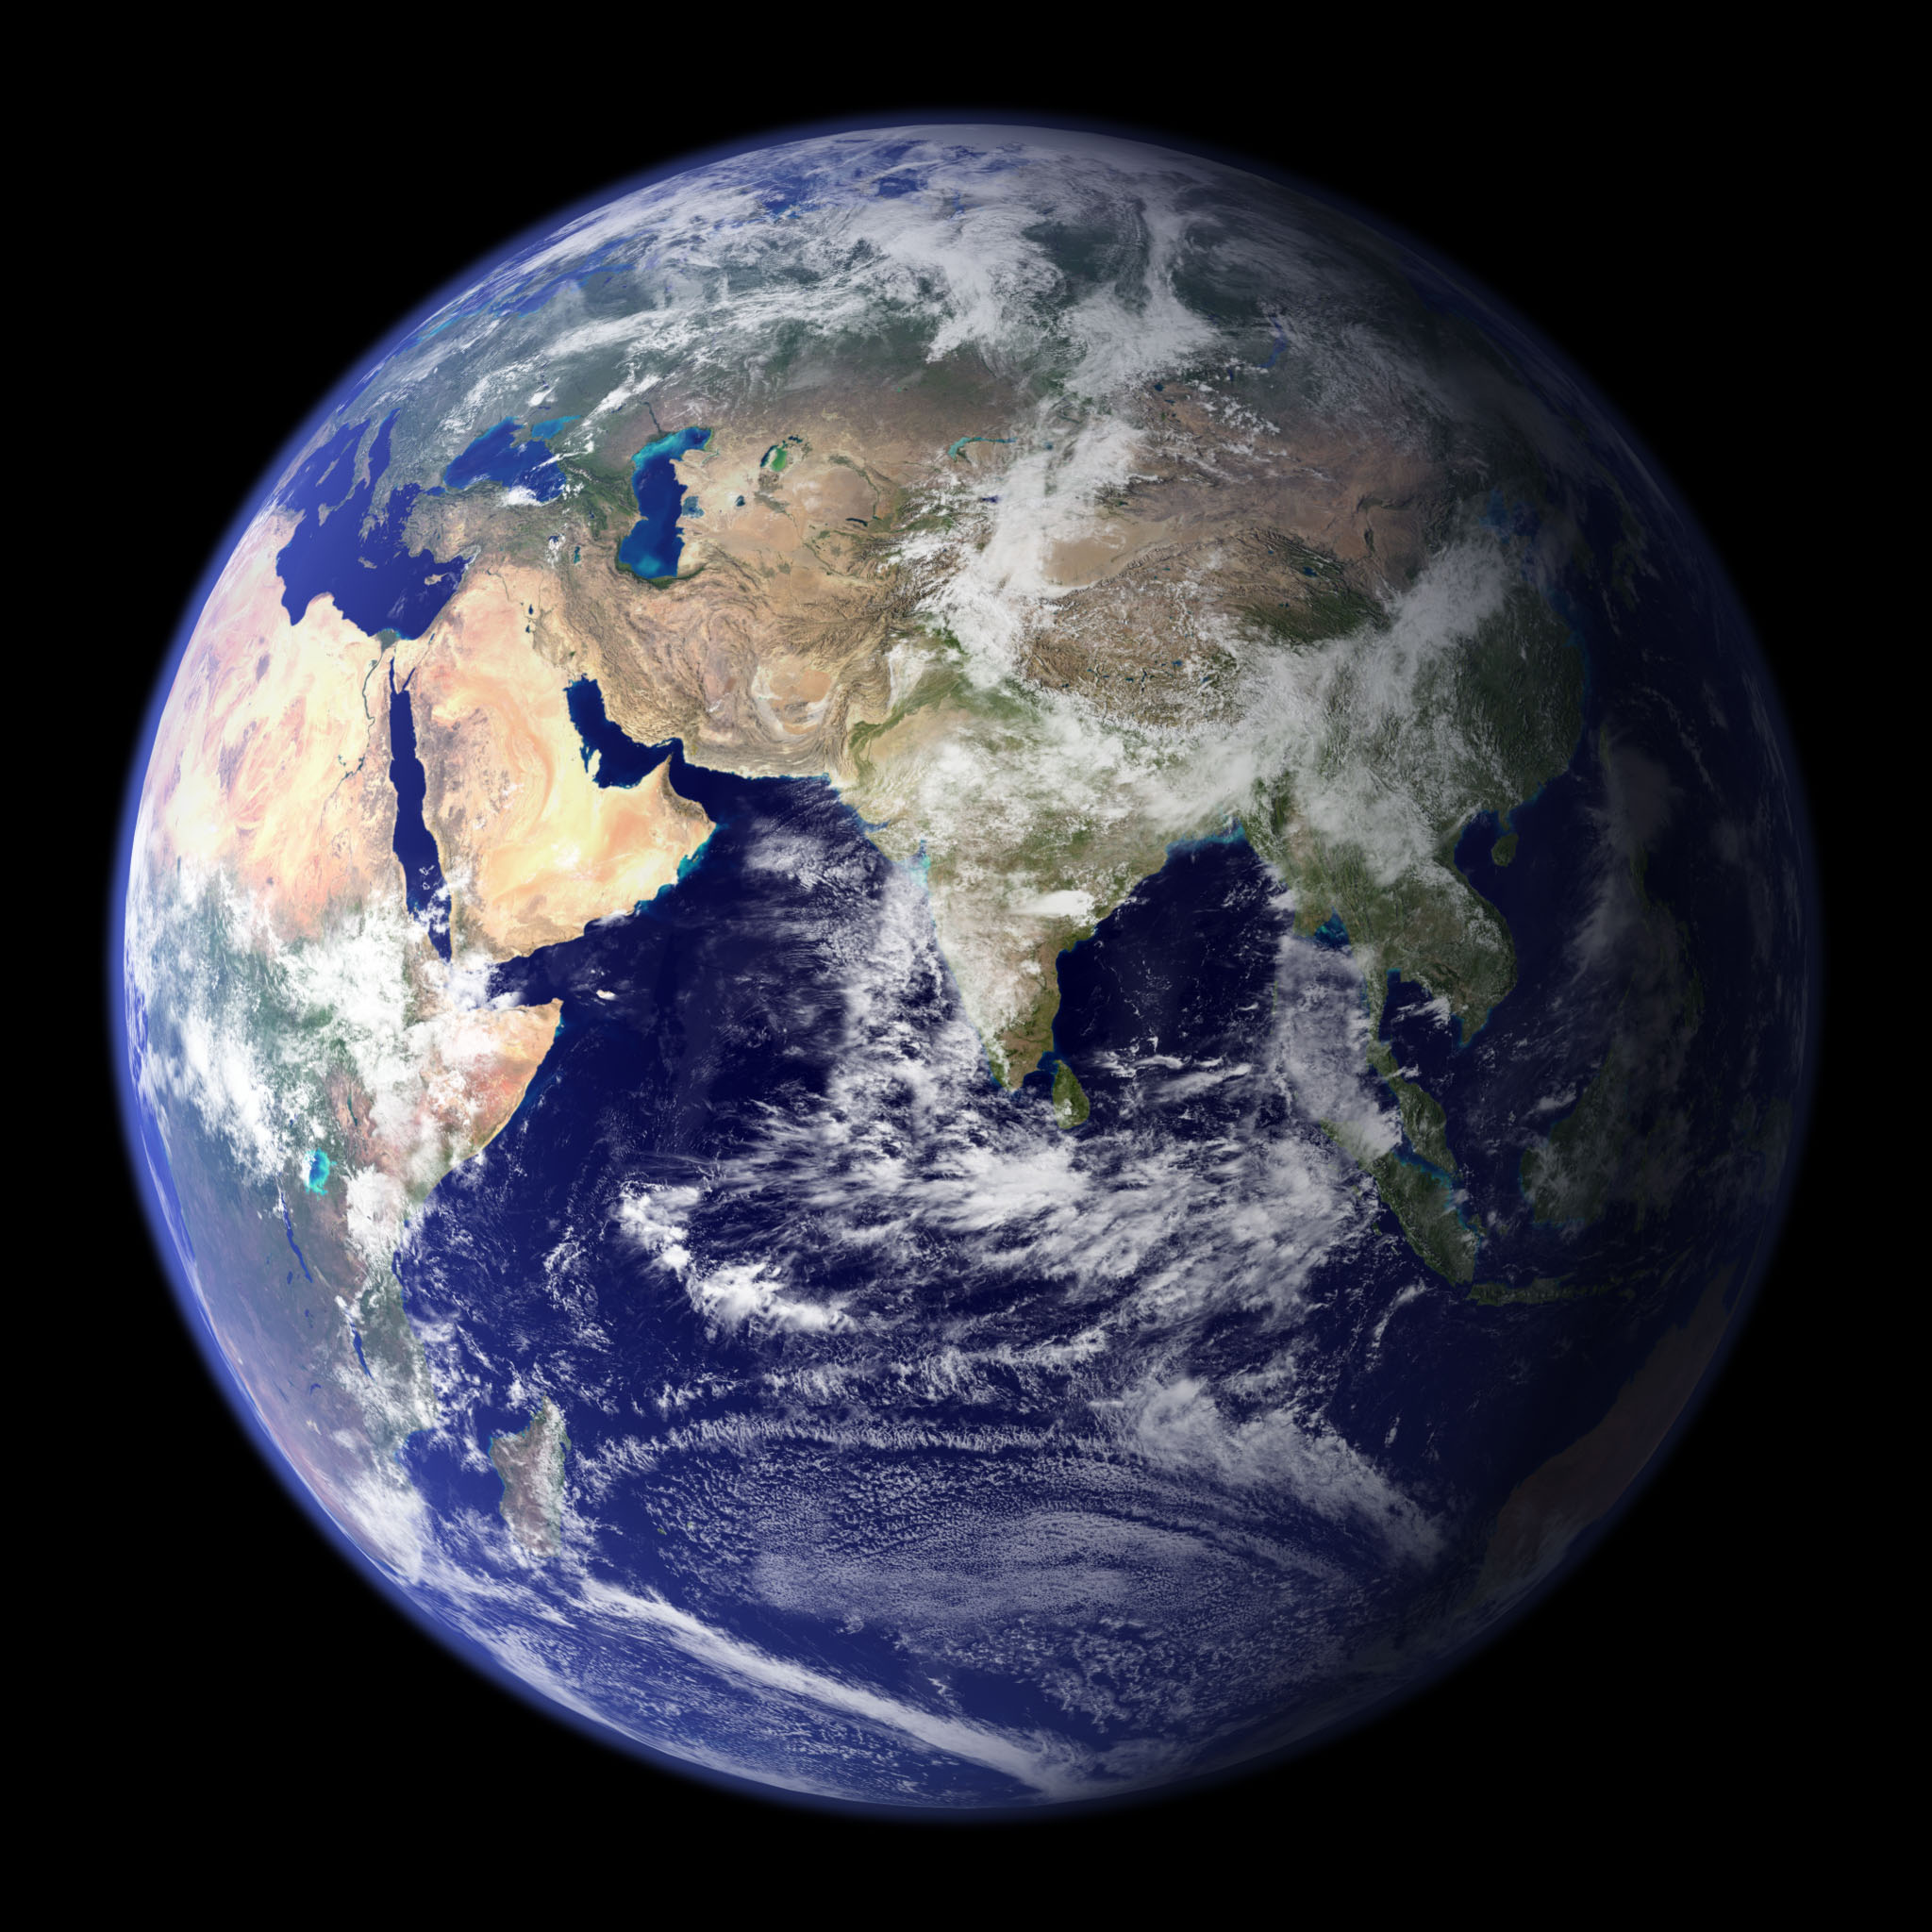
\includegraphics[width=0.3\textwidth]{Earth.jpg}
  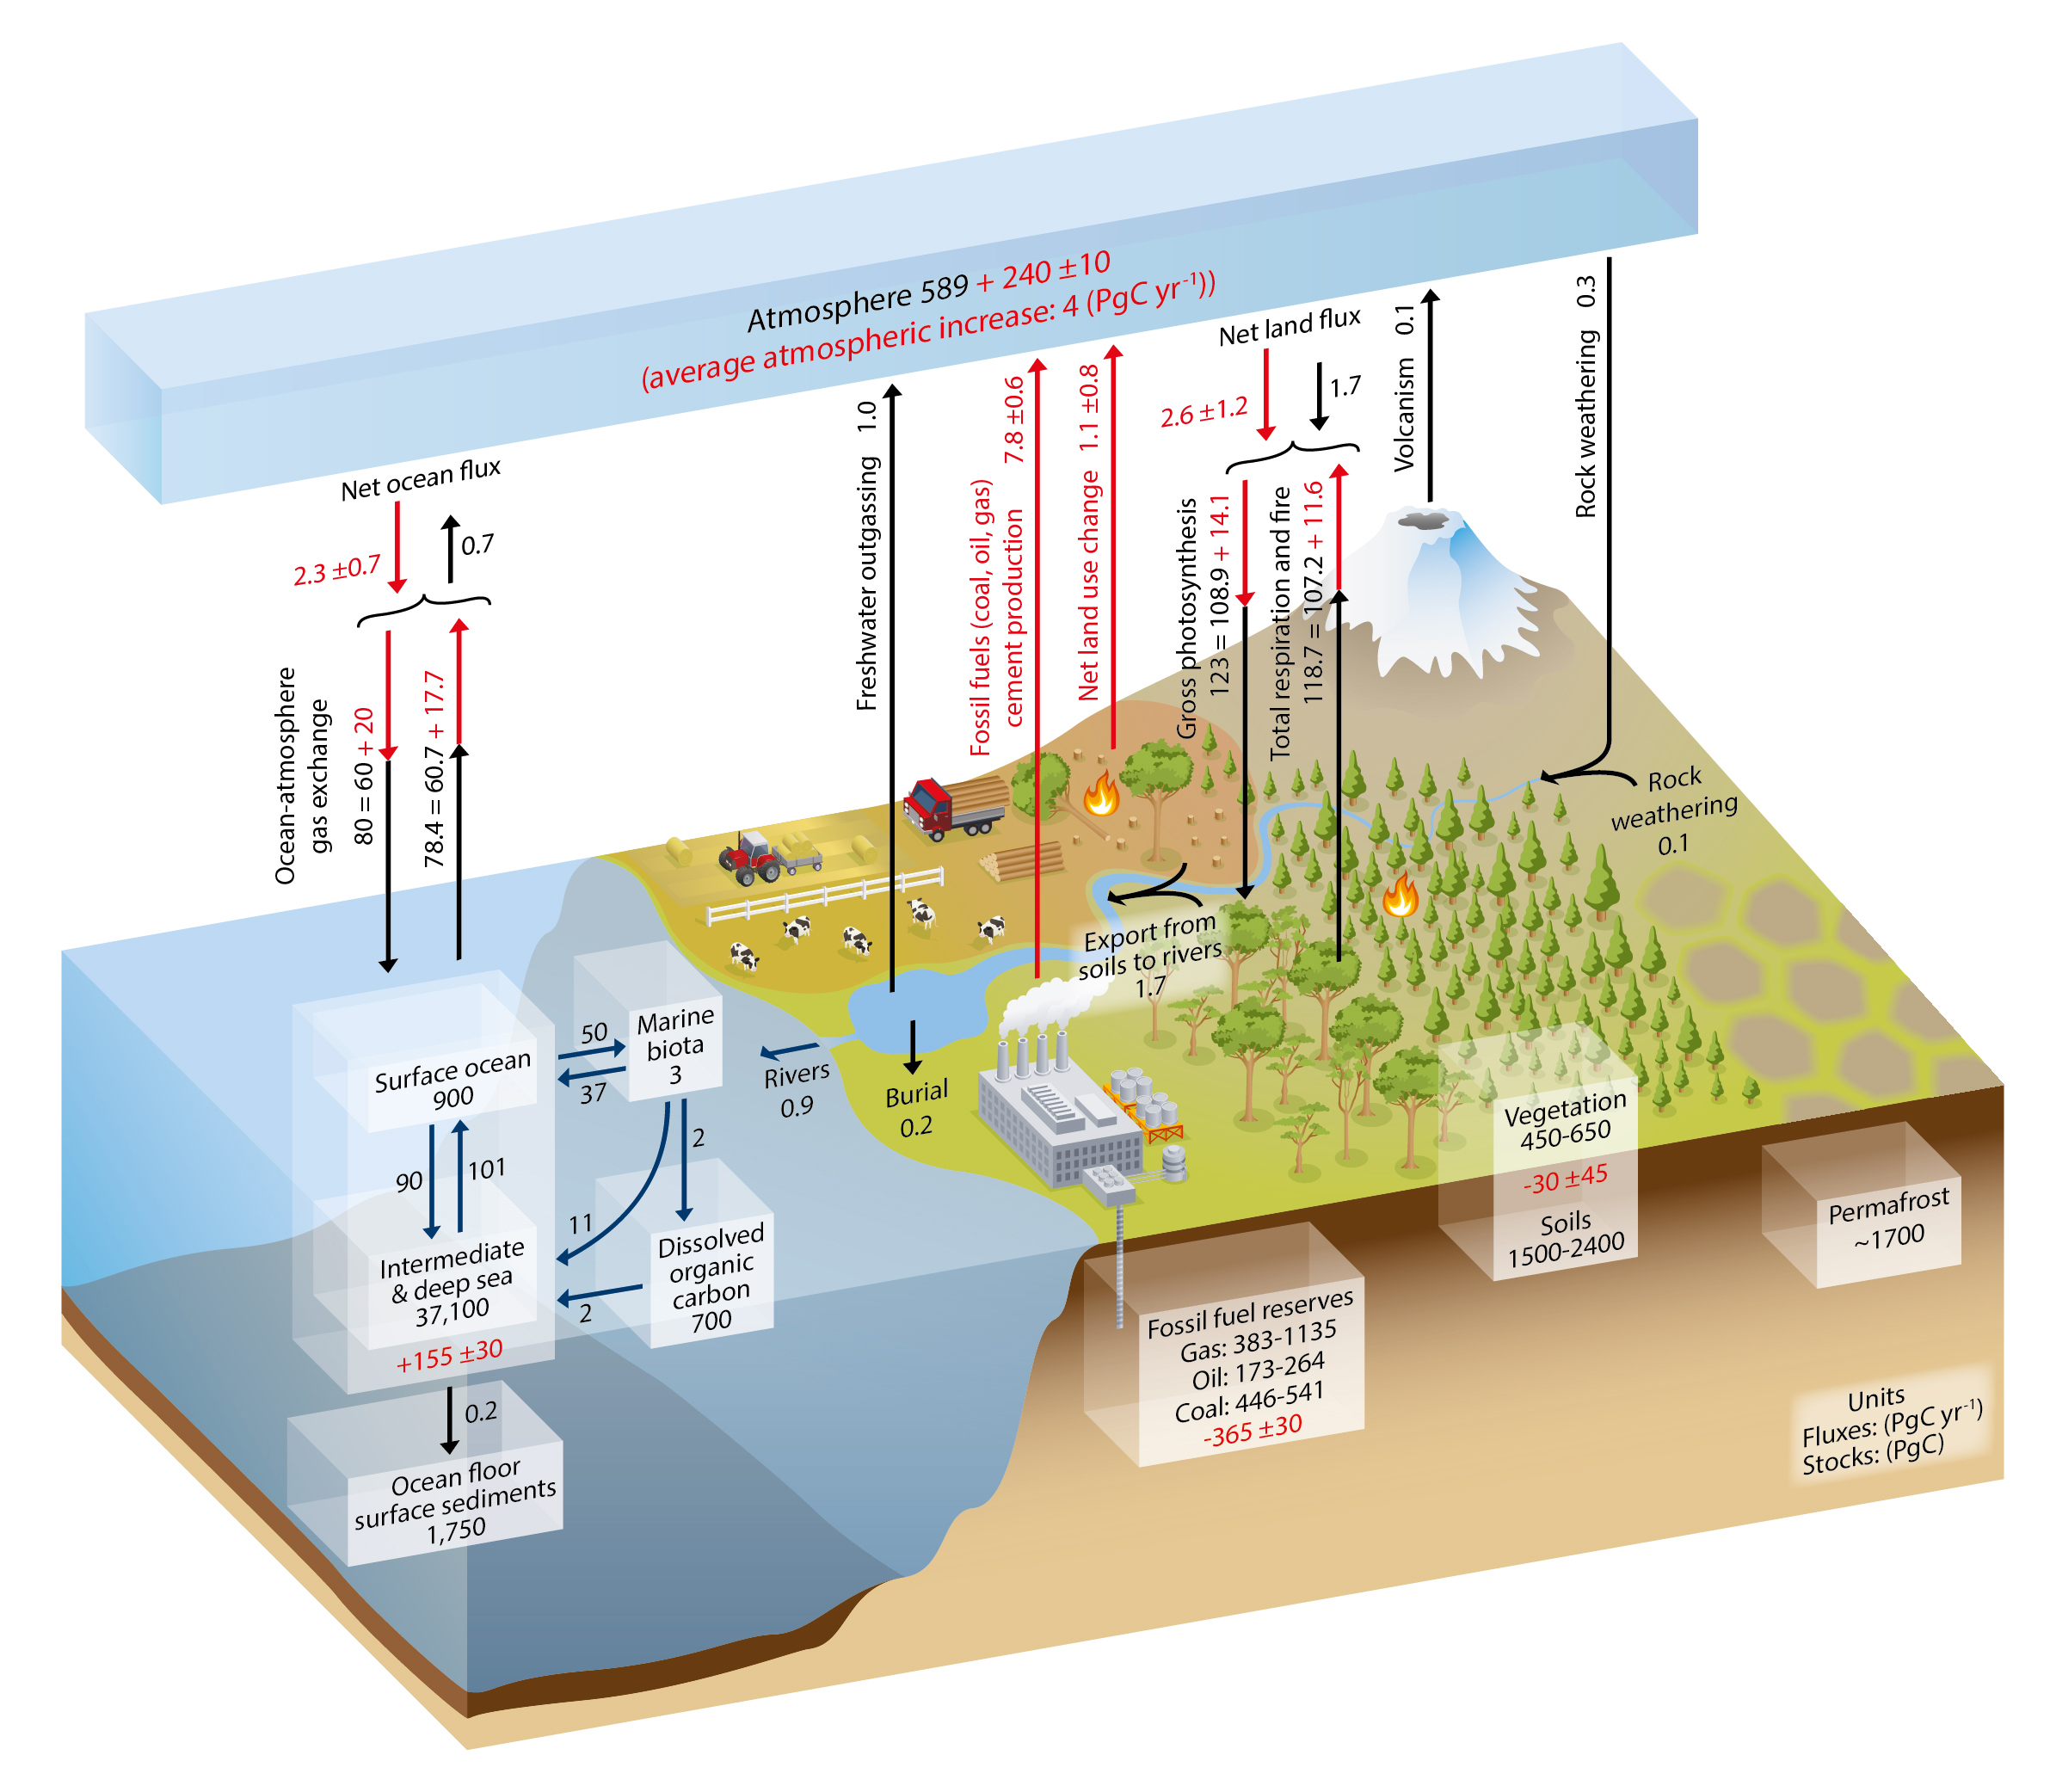
\includegraphics[width=0.3\textwidth]{cCycleIPCC.jpg}
  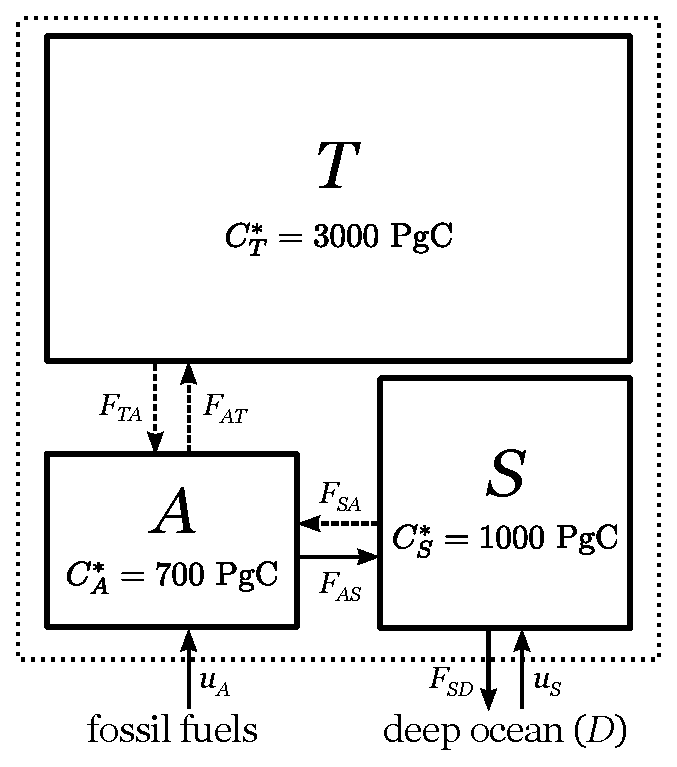
\includegraphics[width=0.35\textwidth]{model2.pdf}

\end{frame}
%%%%%%%%%%%%%%%%%%%%%%%%%%%%%%%%%%%%%%%%%%%%%%%%%%%%%%%%%%%%%%%%%%%%%%%%%%%%%%%%%%%%%%%%%%%%%%%%%%%%%
\subsection{Asking Simpler Questions}
%%%%%%%%%%%%%%%%%%%%%%%%%%%%%%%%%%%%%%%%%%%%%%%%%%%%%%%%%%%%%%%%%%%%%%%%%%%%%%%%%%%%%%%%%%%%%%%%%%%%%
\begin{frame}
	\frametitle{}
	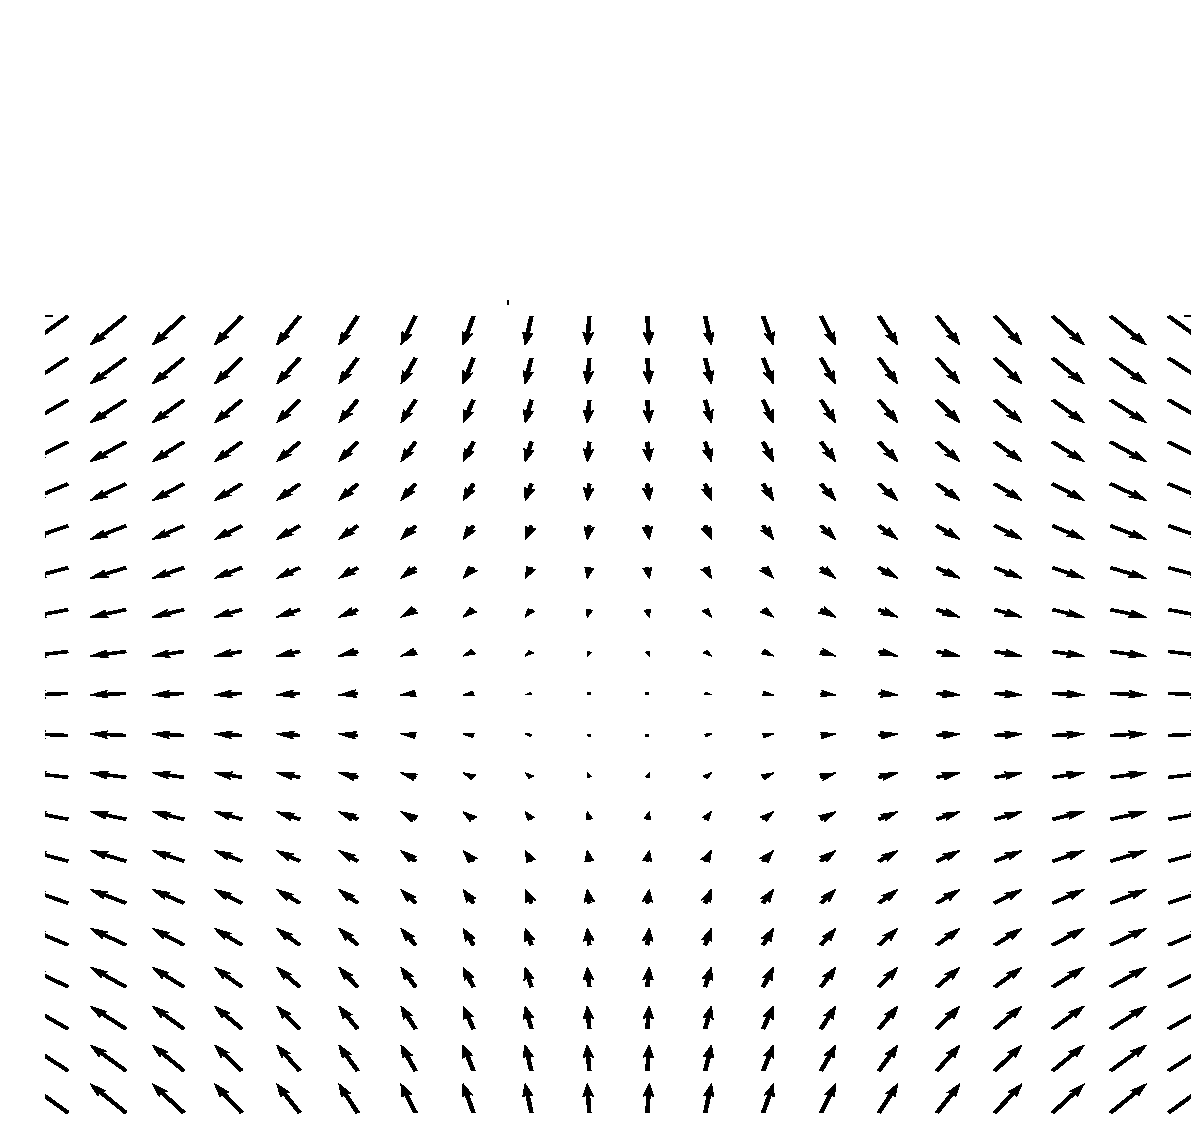
\includegraphics[width=0.9\textwidth]{Solenoidal_vector_field_2.pdf}
\end{frame}
%%%%%%%%%%%%%%%%%%%%%%%%%%%%%%%%%%%%%%%%%%%%%%%%%%%%%%%%%%%%%%%%%%%%%%%%%%%%%%%%%%%%%%%%%%%%%%%%%%%%%
\begin{frame}
	\frametitle{}
	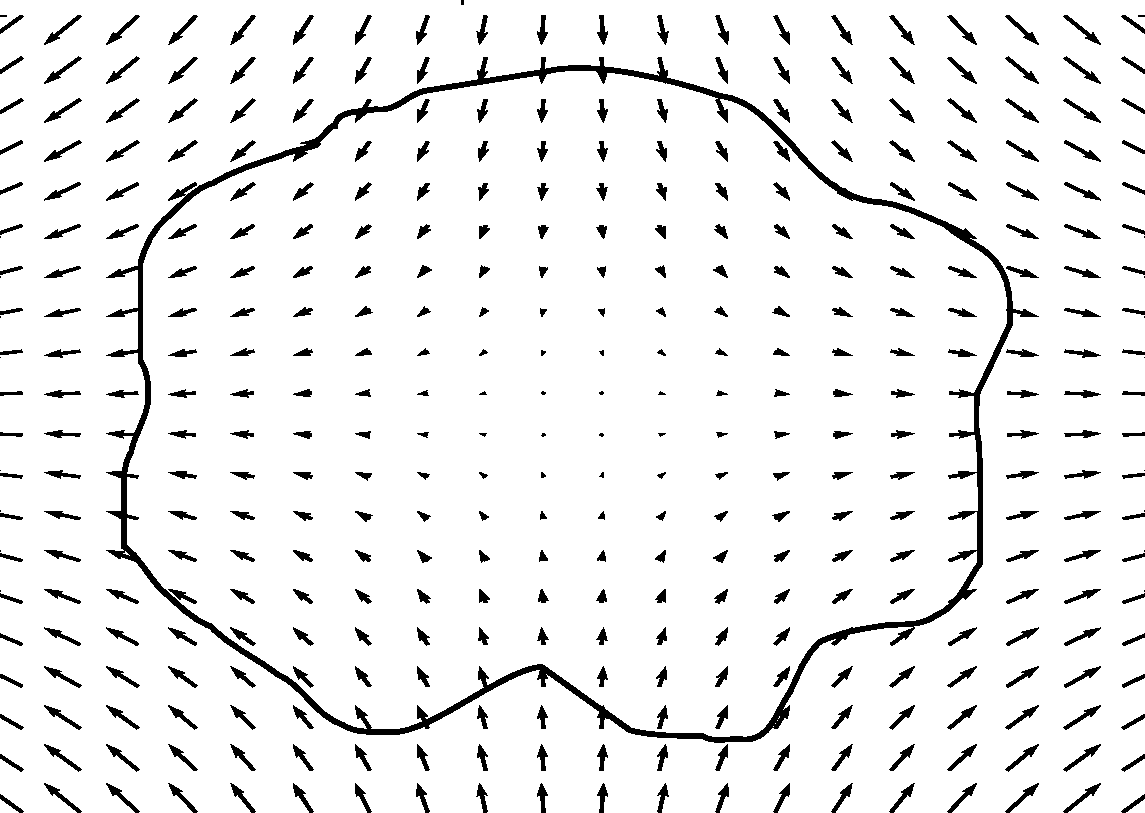
\includegraphics[width=0.9\textwidth]{VectorFieldWithOnePool.pdf}
\end{frame}
%%%%%%%%%%%%%%%%%%%%%%%%%%%%%%%%%%%%%%%%%%%%%%%%%%%%%%%%%%%%%%%%%%%%%%%%%%%%%%%%%%%%%%%%%%%%%%%%%%%%%
\begin{frame}
	\frametitle{}
	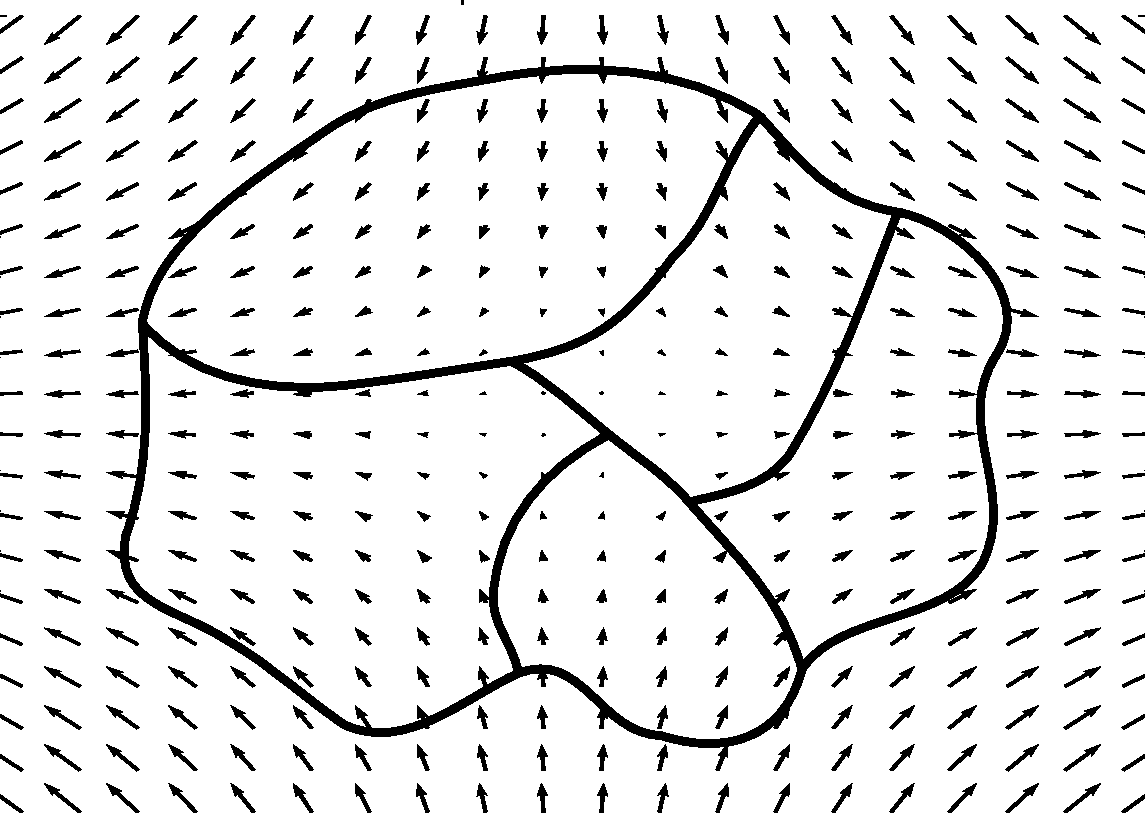
\includegraphics[width=0.9\textwidth]{VectorFieldWithOnePoolAndSubpools.pdf}
\end{frame}
%%%%%%%%%%%%%%%%%%%%%%%%%%%%%%%%%%%%%%%%%%%%%%%%%%%%%%%%%%%%%%%%%%%%%%%%%%%%%%%%%%%%%%%%%%%%%%%%%%%%%
\begin{frame}
	\frametitle{}
	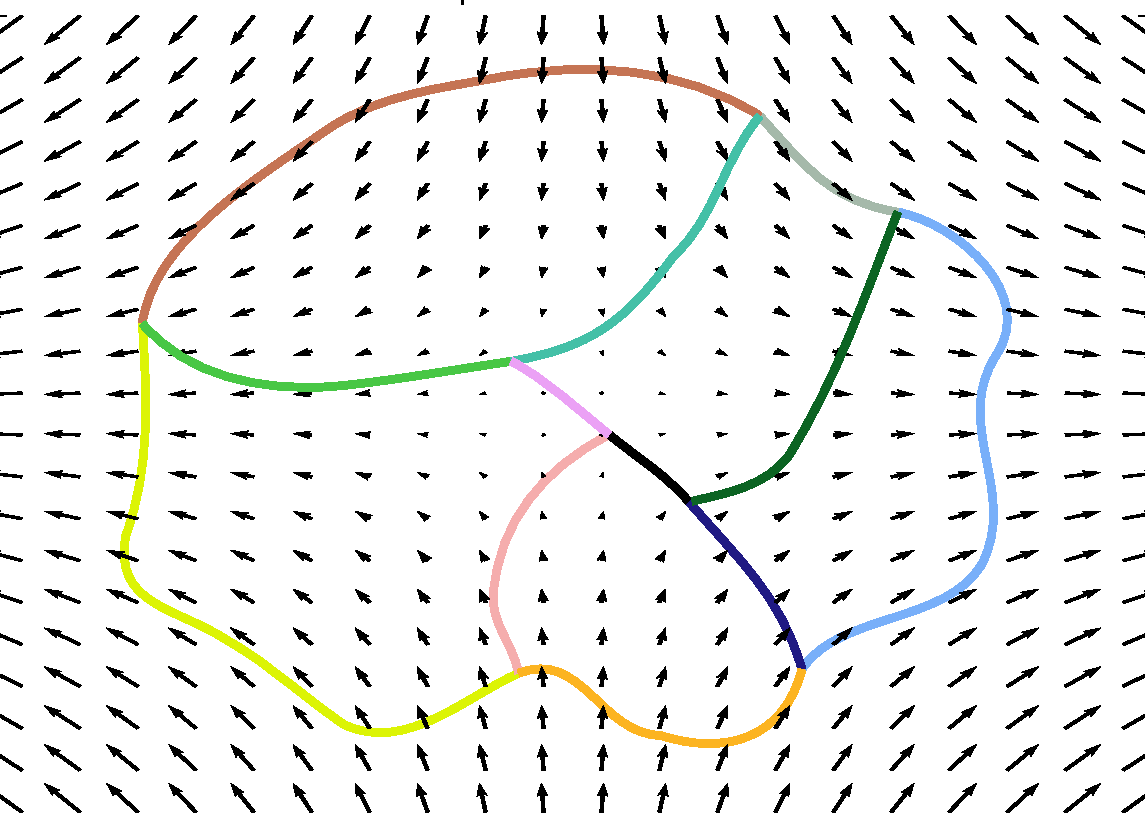
\includegraphics[width=0.9\textwidth]{VectorFieldWithOnePoolAndSubpoolsAndColoredBoundaries.pdf}
\end{frame}
%%%%%%%%%%%%%%%%%%%%%%%%%%%%%%%%%%%%%%%%%%%%%%%%%%%%%%%%%%%%%%%%%%%%%%%%%%%%%%%%%%%%%%%%%%%%%%%%%%%%%
\begin{frame}
	\frametitle{}
	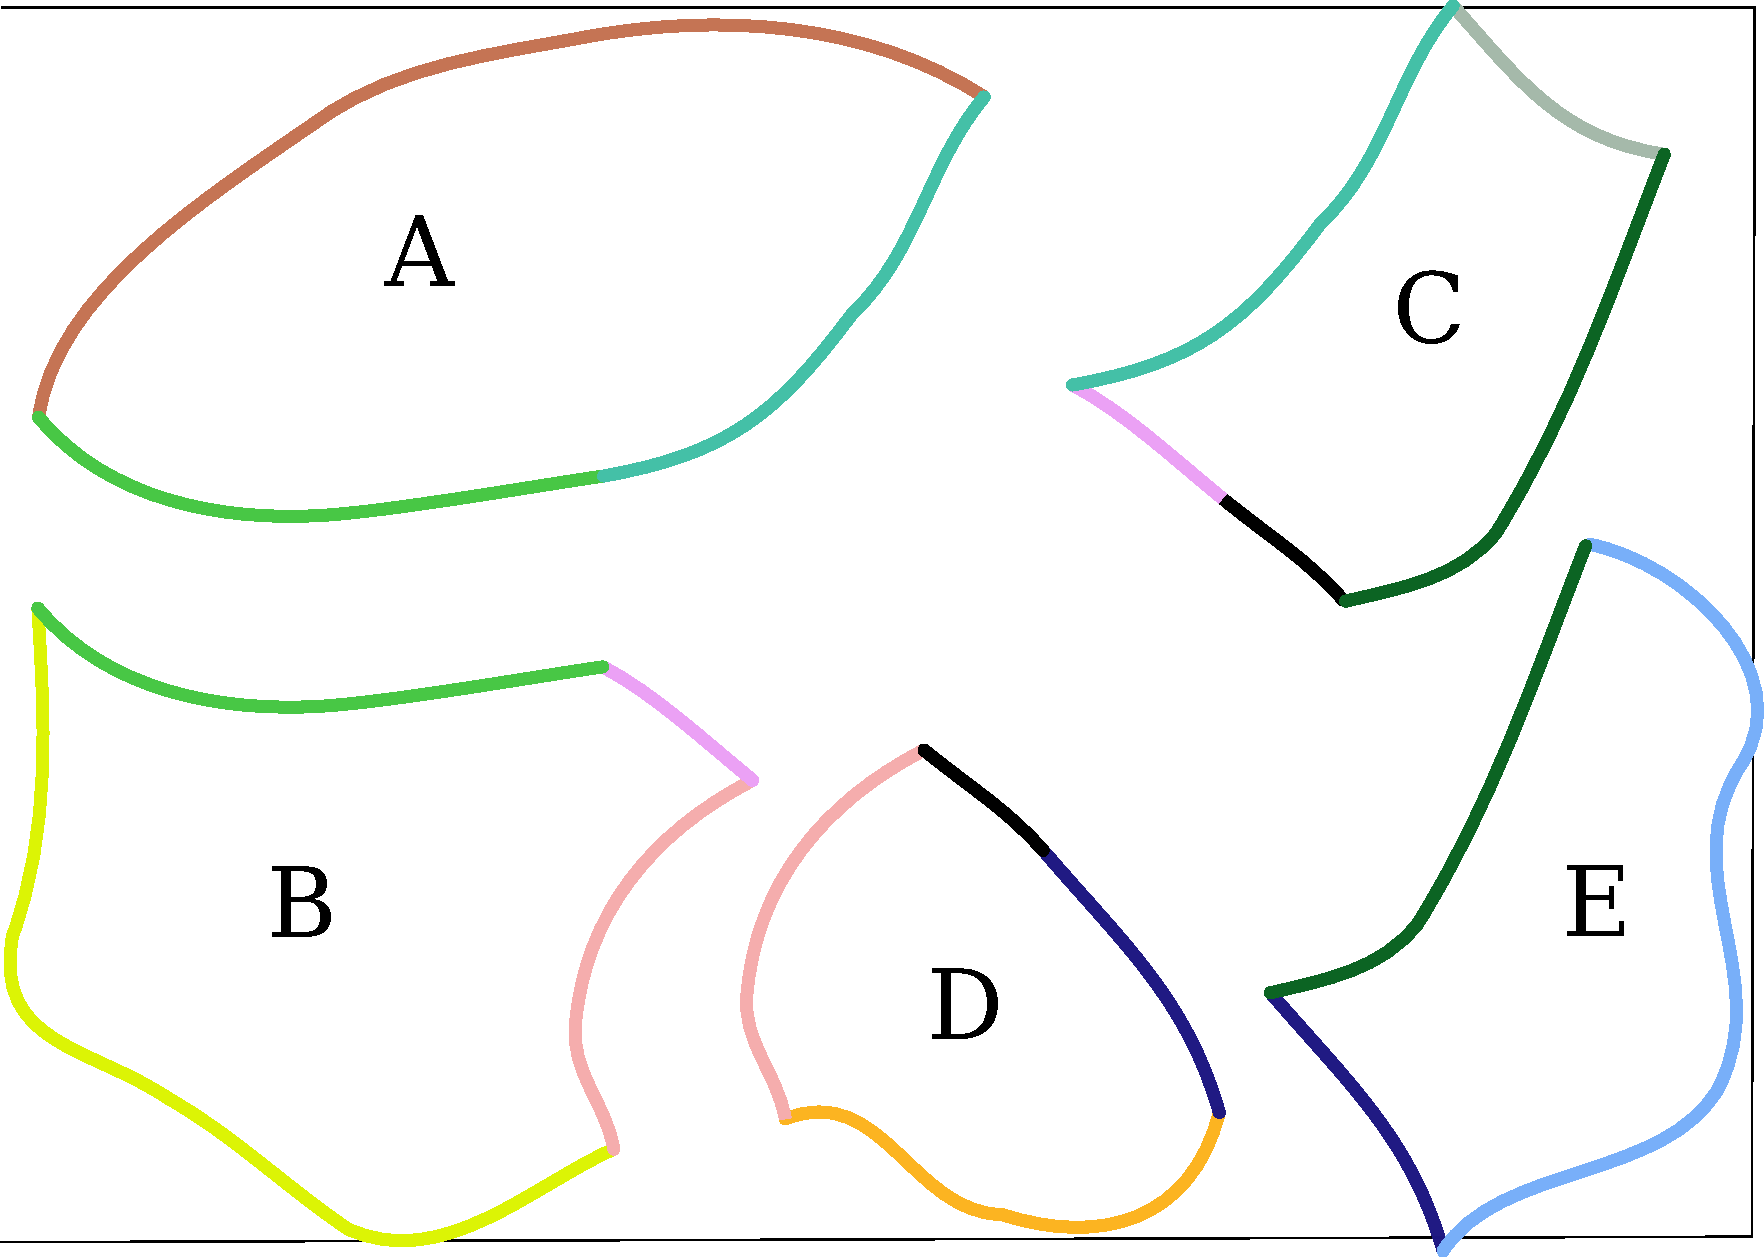
\includegraphics[width=0.9\textwidth]{SubpoolsAndColoredBoundaries.pdf}
\end{frame}
%%%%%%%%%%%%%%%%%%%%%%%%%%%%%%%%%%%%%%%%%%%%%%%%%%%%%%%%%%%%%%%%%%%%%%%%%%%%%%%%%%%%%%%%%%%%%%%%%%%%%
\begin{frame}
	\frametitle{}
	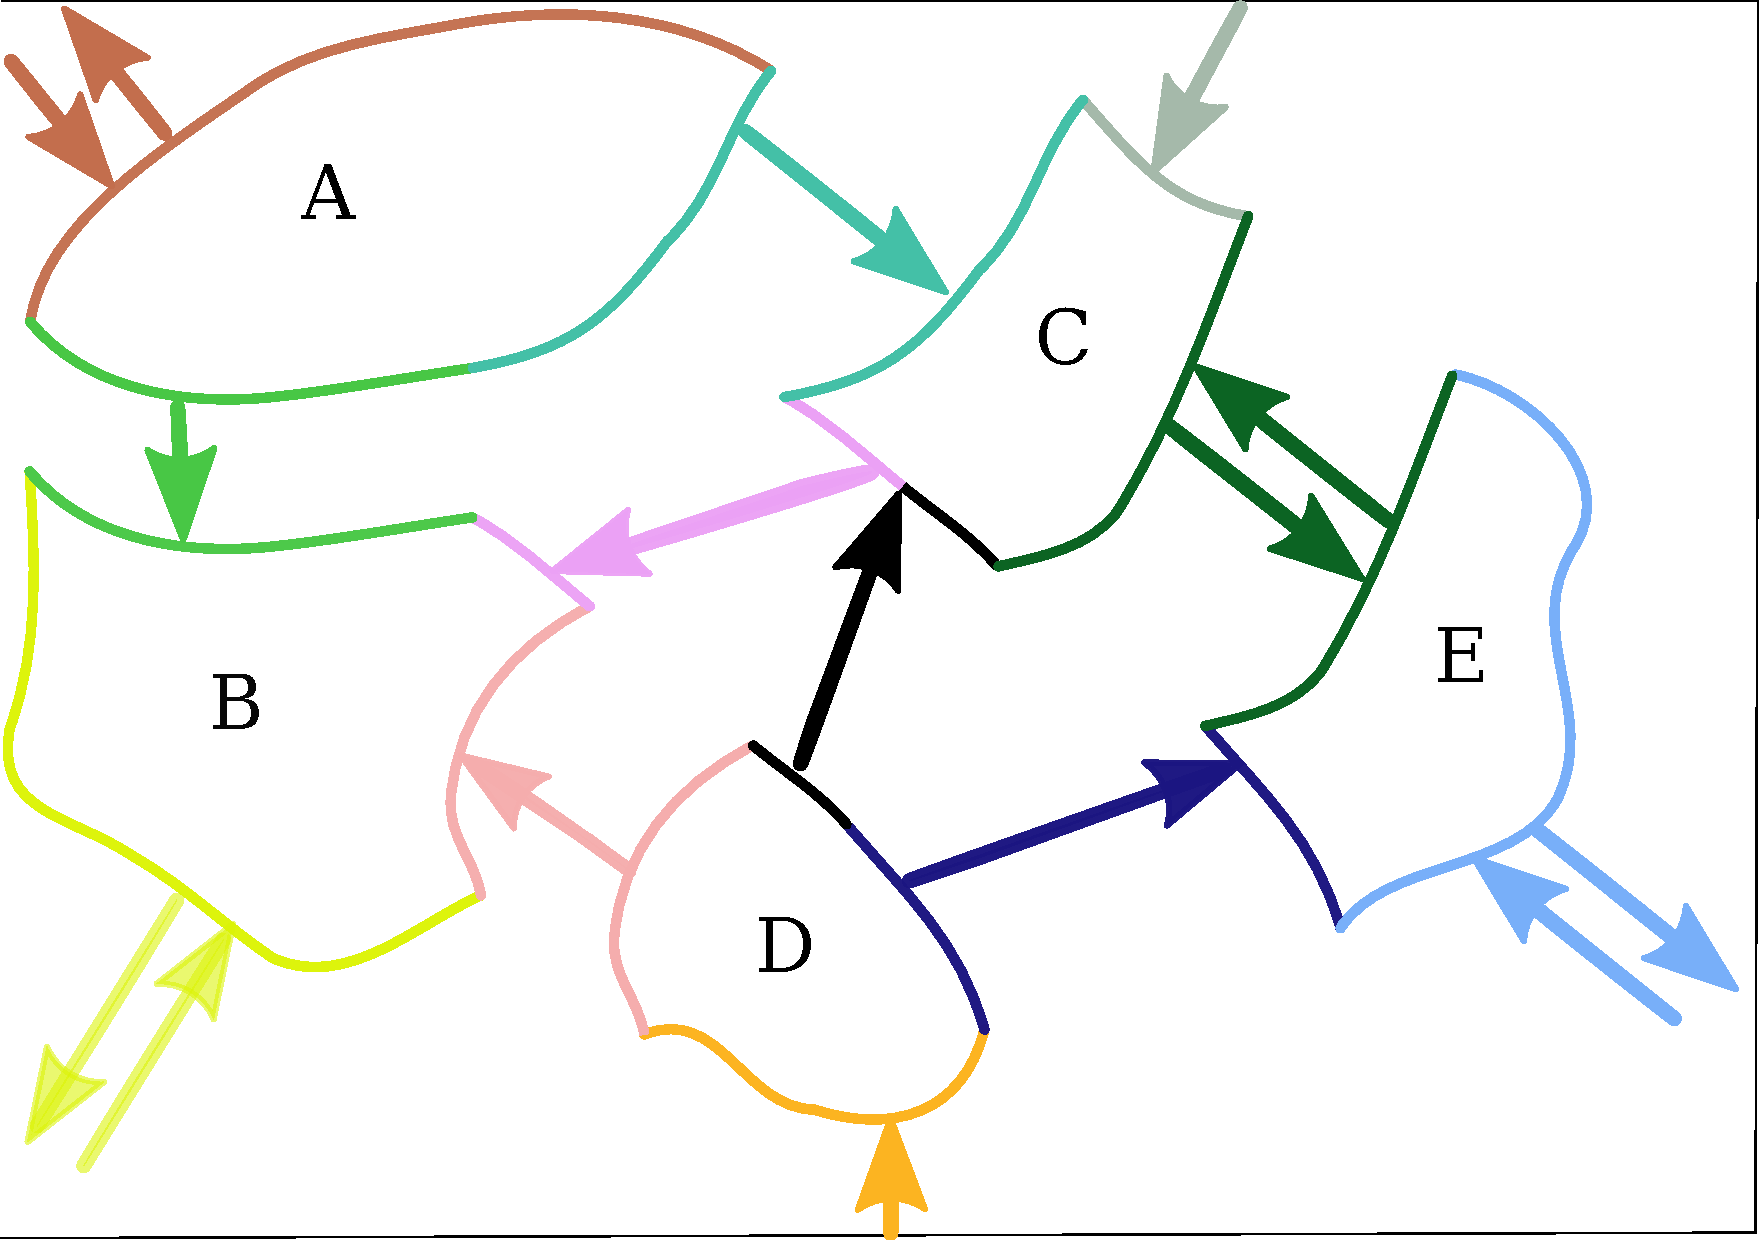
\includegraphics[width=0.9\textwidth]{SubpoolsAndColoredBoundariesAndArrows.pdf}
\end{frame}
%%%%%%%%%%%%%%%%%%%%%%%%%%%%%%%%%%%%%%%%%%%%%%%%%%%%%%%%%%%%%%%%%%%%%%%%%%%%%%%%%%%%%%%%%%%%%%%%%%%%%
\begin{frame}
	\frametitle{}
	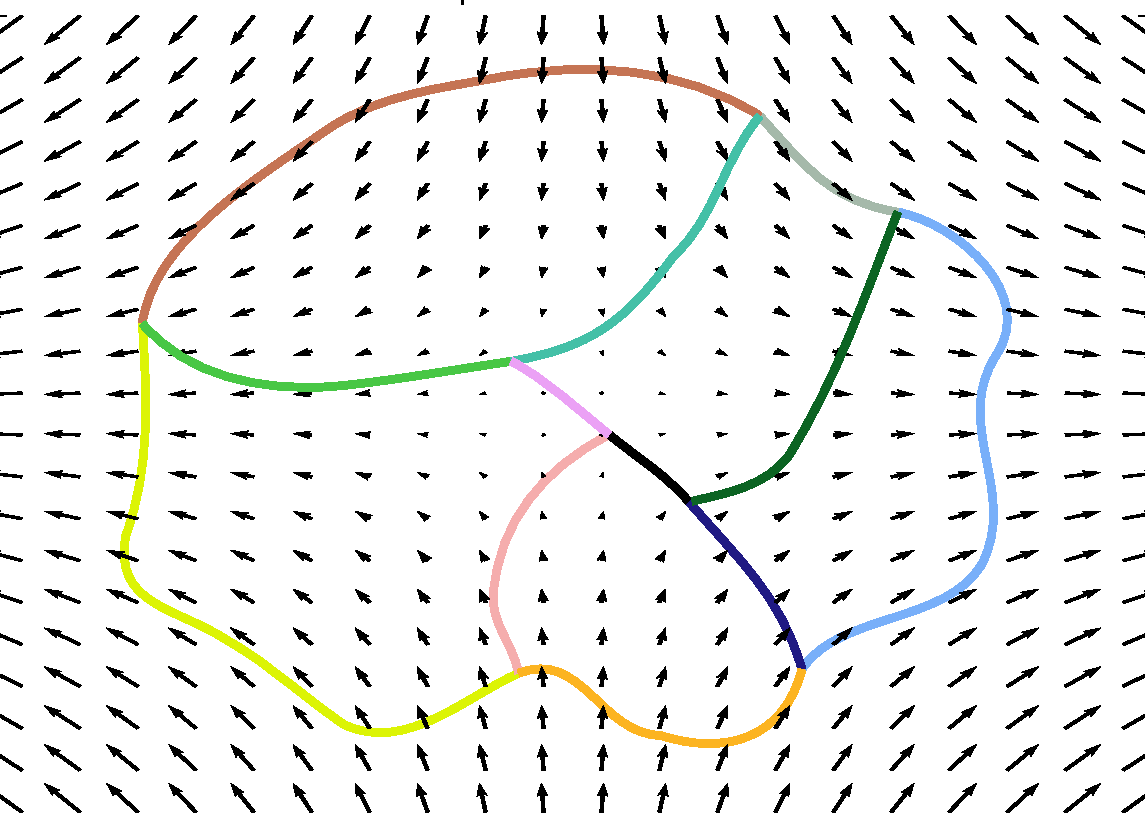
\includegraphics[width=0.45\textwidth]{VectorFieldWithOnePoolAndSubpoolsAndColoredBoundaries.pdf}
	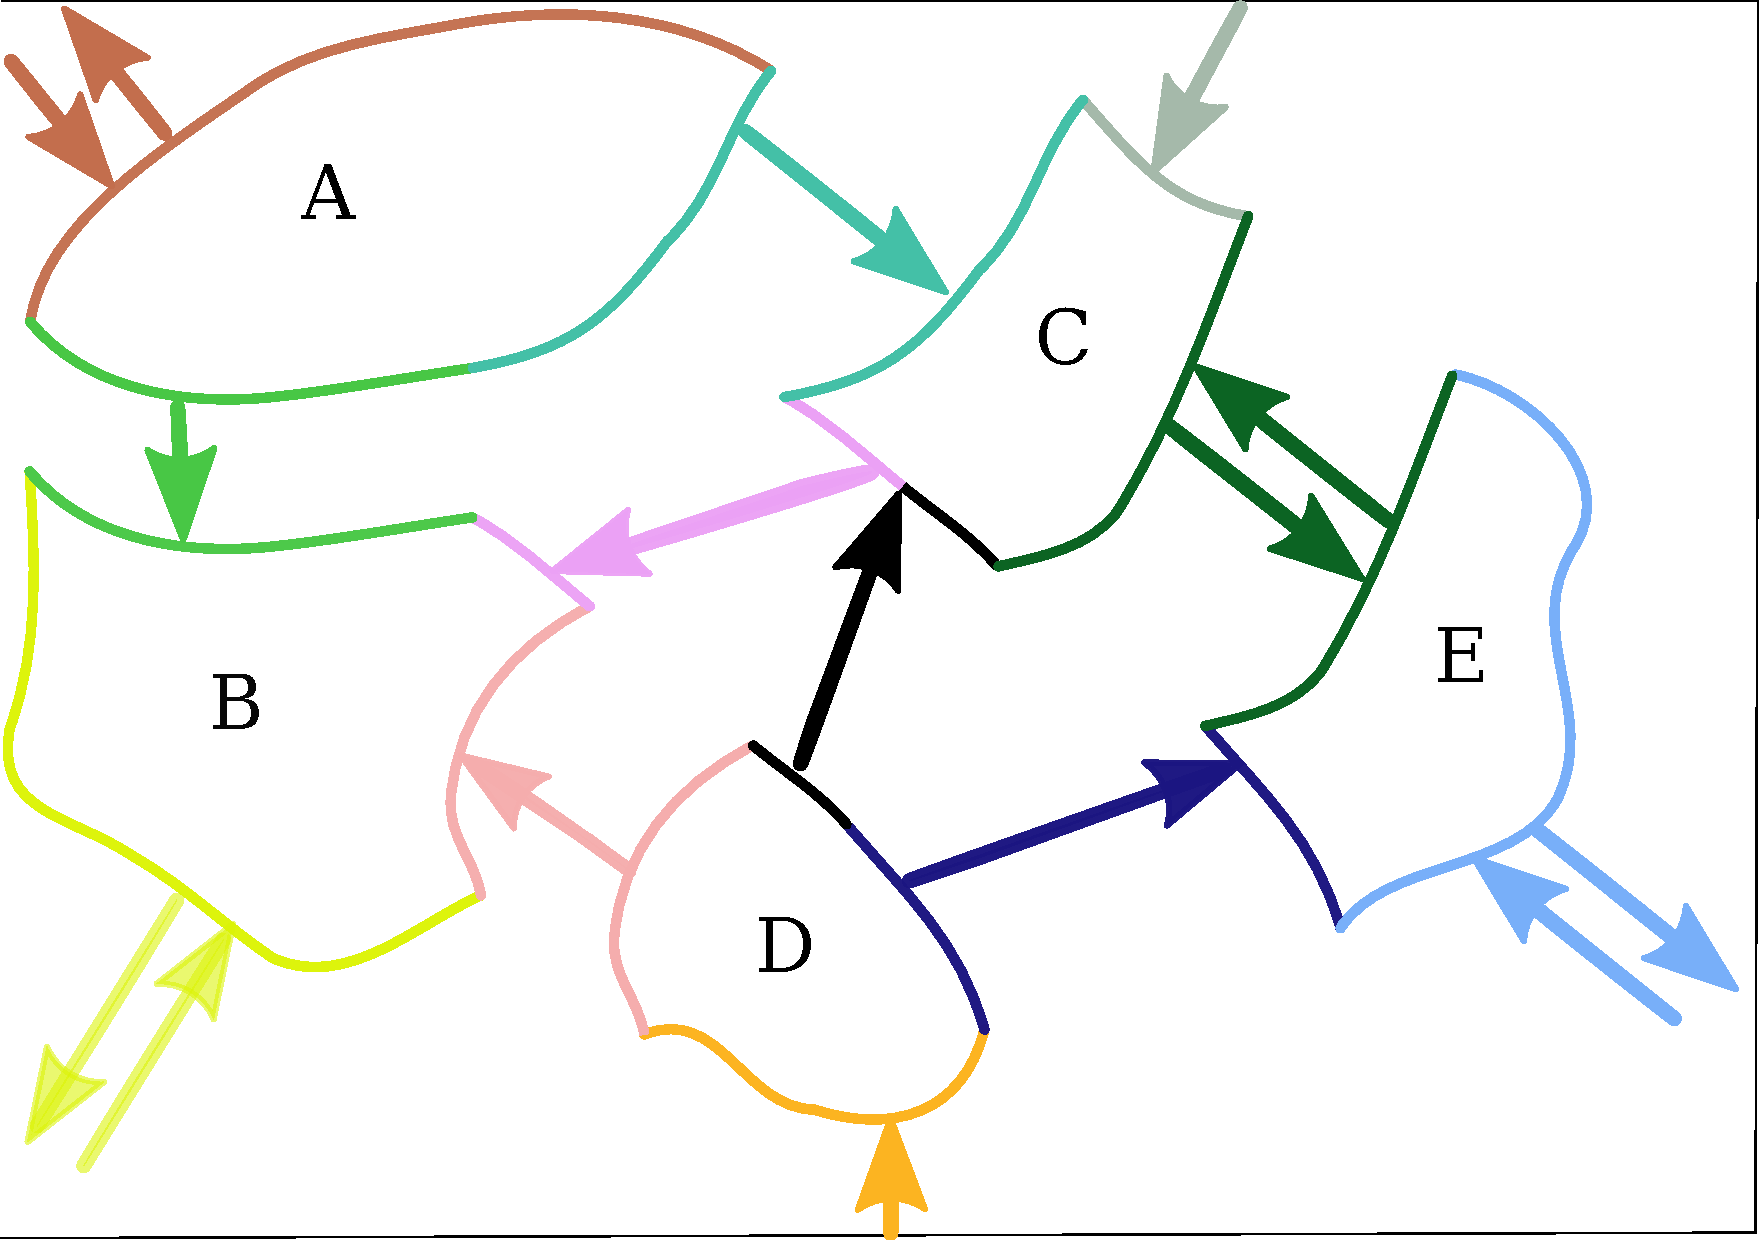
\includegraphics[width=0.45\textwidth]{SubpoolsAndColoredBoundariesAndArrows.pdf}
\end{frame}
%%%%%%%%%%%%%%%%%%%%%%%%%%%%%%%%%%%%%%%%%%%%%%%%%%%%%%%%%%%%%%%%%%%%%%%%%%%%%%%%%%%%%%%%%%%%%%%%%%%%%
\begin{frame}
	\frametitle{}
	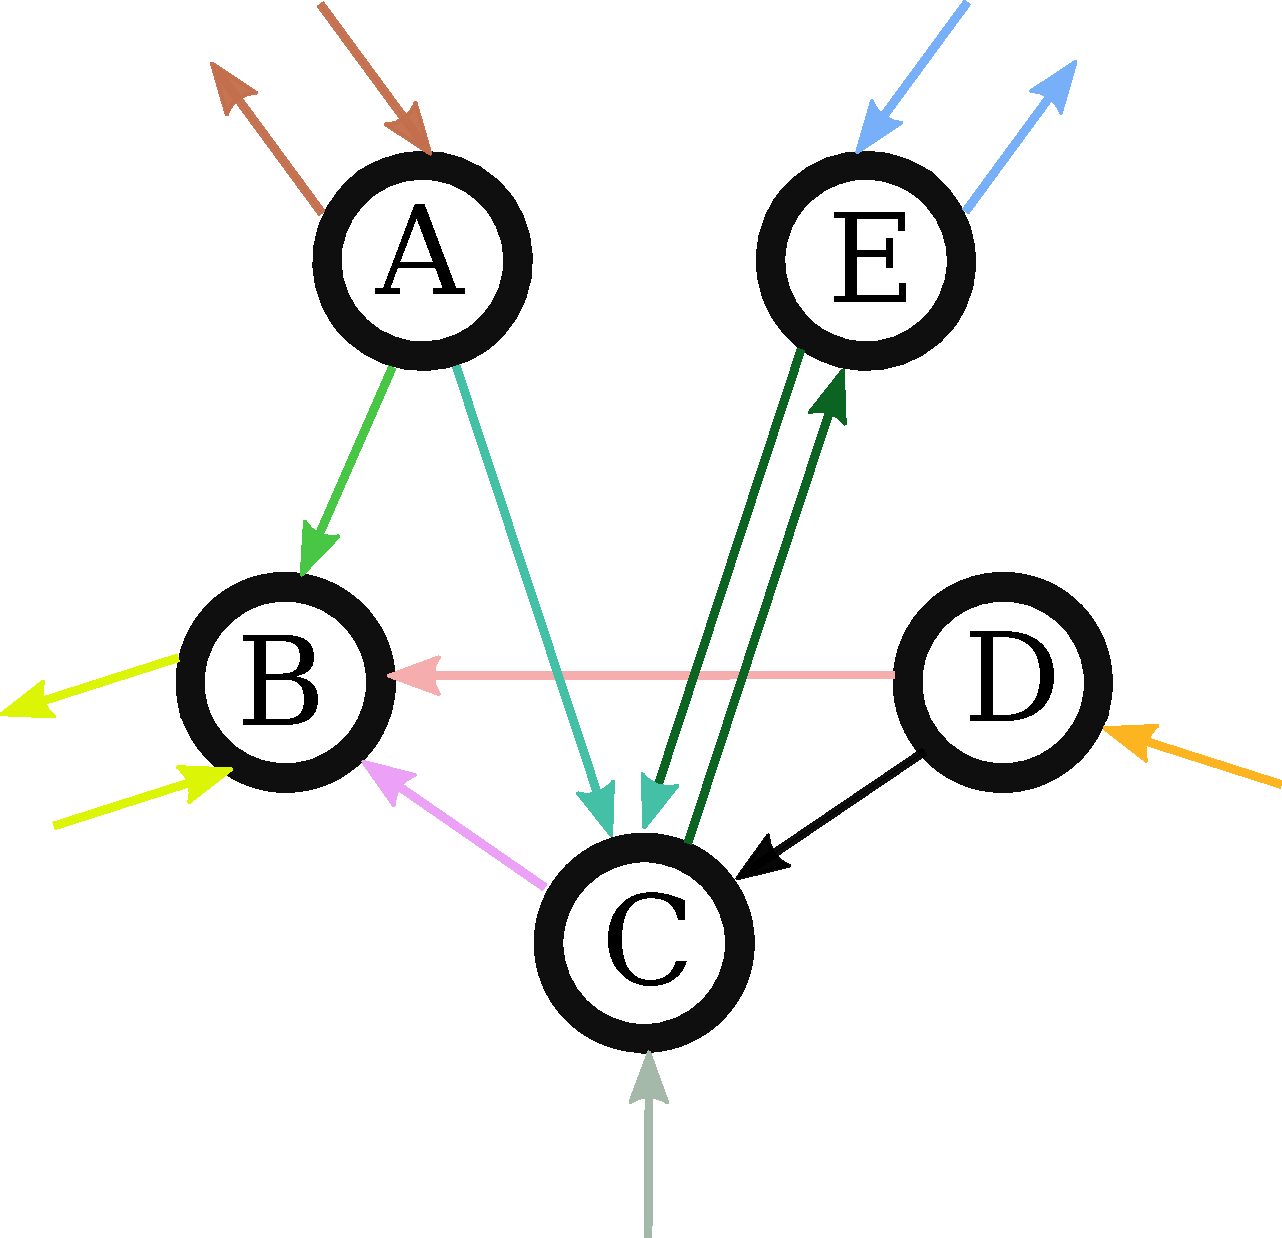
\includegraphics[height=0.9\textheight]{RoundPoolscColoredArrows.pdf}
\end{frame}
%%%%%%%%%%%%%%%%%%%%%%%%%%%%%%%%%%%%%%%%%%%%%%%%%%%%%%%%%%%%%%%%%%%%%%%%%%%%%%%%%%%%%%%%%%%%%%%%%%%%%
\begin{frame}
	\frametitle{}
	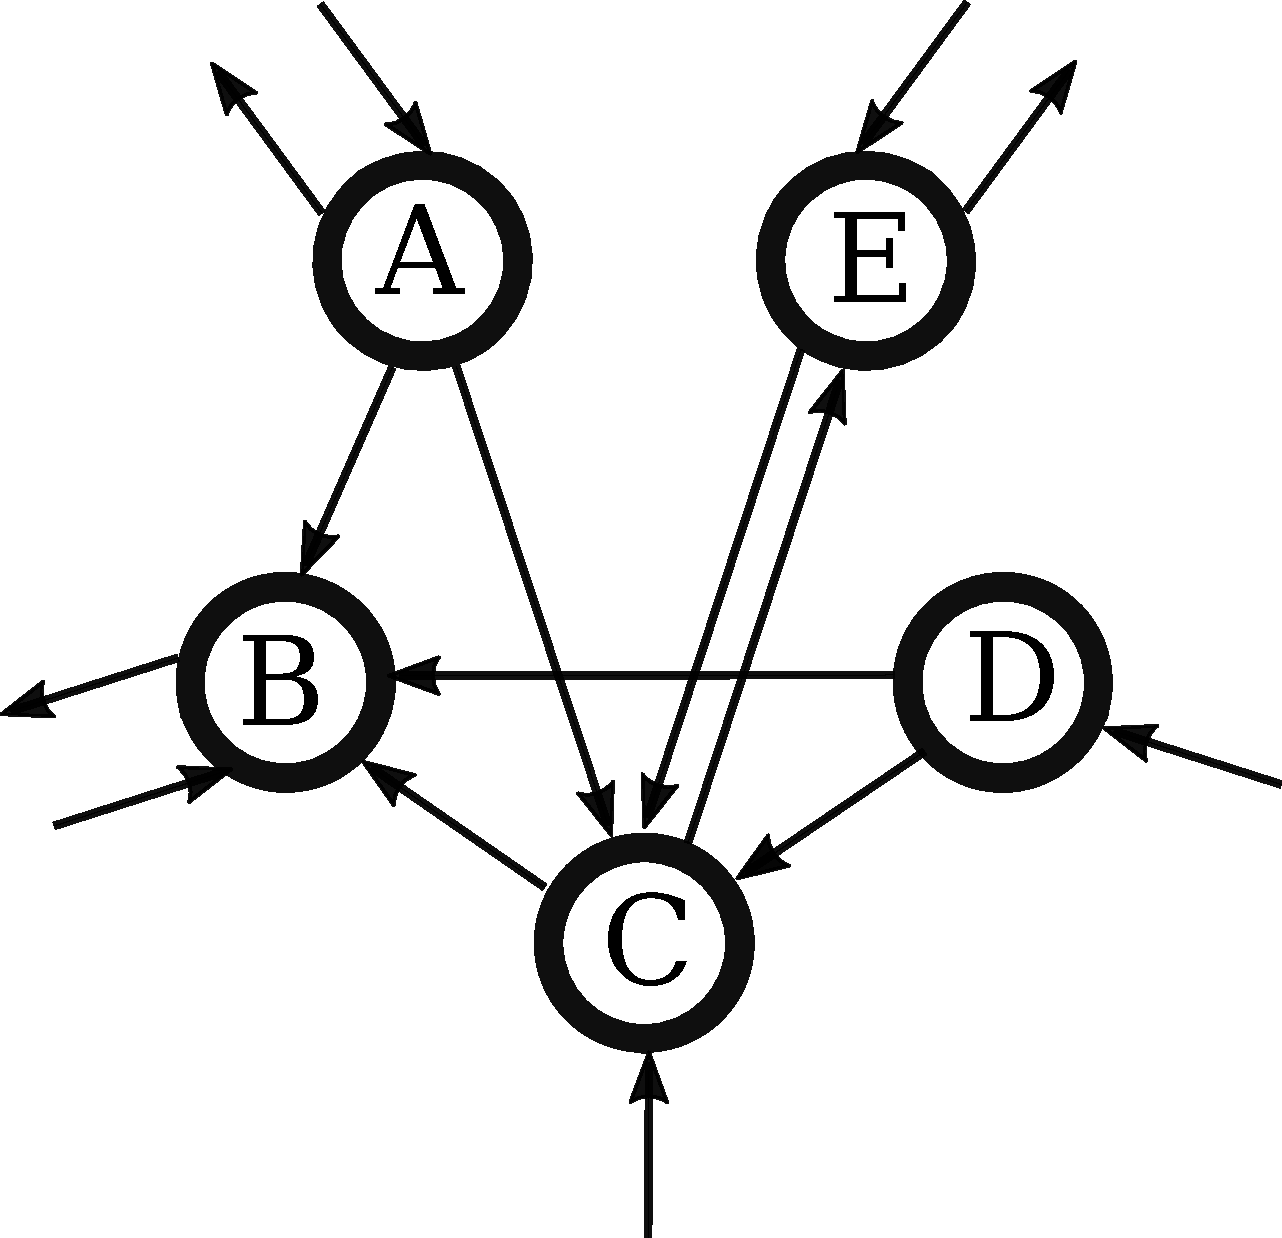
\includegraphics[height=0.9\textheight]{RoundPoolsBlackArrows.pdf}
\end{frame}
%%%%%%%%%%%%%%%%%%%%%%%%%%%%%%%%%%%%%%%%%%%%%%%%%%%%%%%%%%%%%%%%%%%%%%%%%%%%%%%%%%%%%%%%%%%%%%%%%%%%%
\begin{frame}
  
\includegraphics[width=0.45\textwidth]{FritzC.pdf}
  
\includegraphics[width=0.45\textwidth]{Open_passport.pdf}
\end{frame}
%%%%%%%%%%%%%%%%%%%%%%%%%%%%%%%%%%%%%%%%%%%%%%%%%%%%%%%%%%%%%%%%%%%%%%%%%%%%%%%%%%%%%%%%%%%%%%%%%%%%%
\begin{frame}
	\frametitle{}
	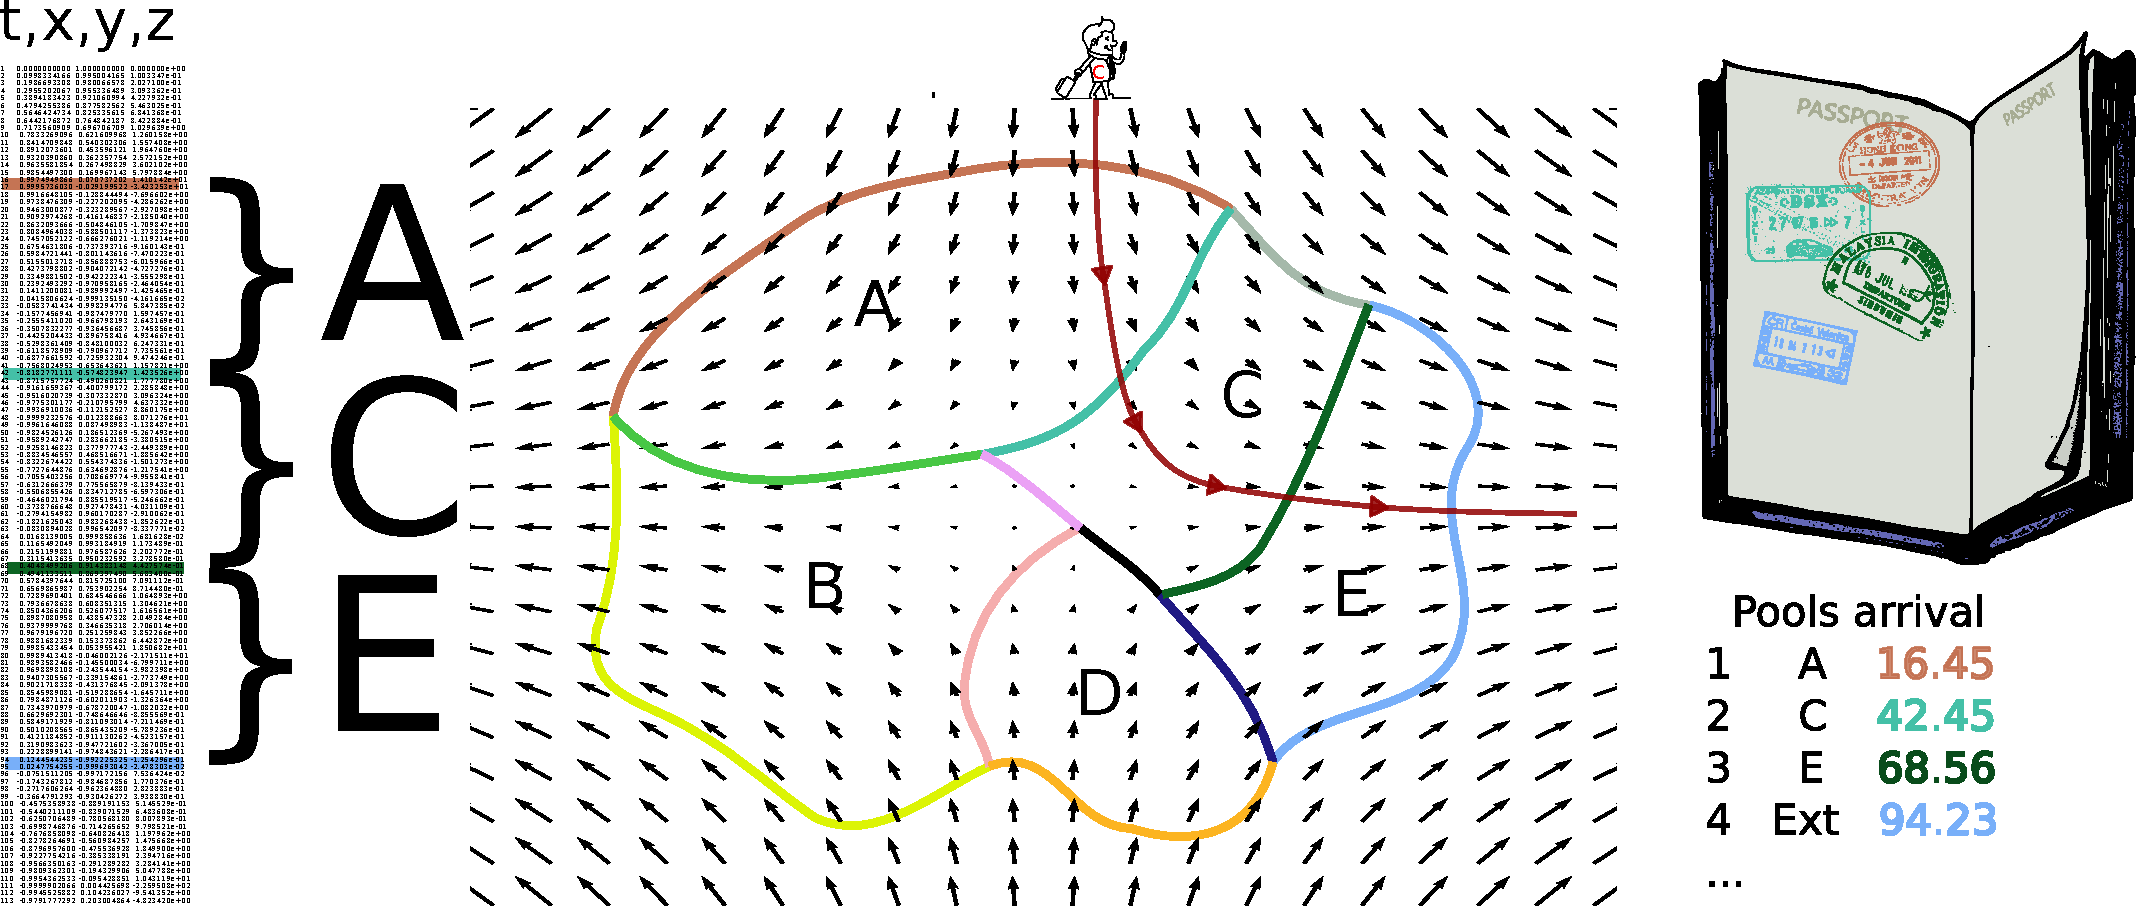
\includegraphics[width=0.9\textwidth]{VectorFieldWithOnePoolAndSubpoolsAndColoredBoundariesAndTrajectory.pdf} 
\end{frame}
%%%%%%%%%%%%%%%%%%%%%%%%%%%%%%%%%%%%%%%%%%%%%%%%%%%%%%%%%%%%%%%%%%%%%%%%%%%%%%%%%%%%%%%%%%%%%%%%%%%%%
\begin{frame}
	\frametitle{}
	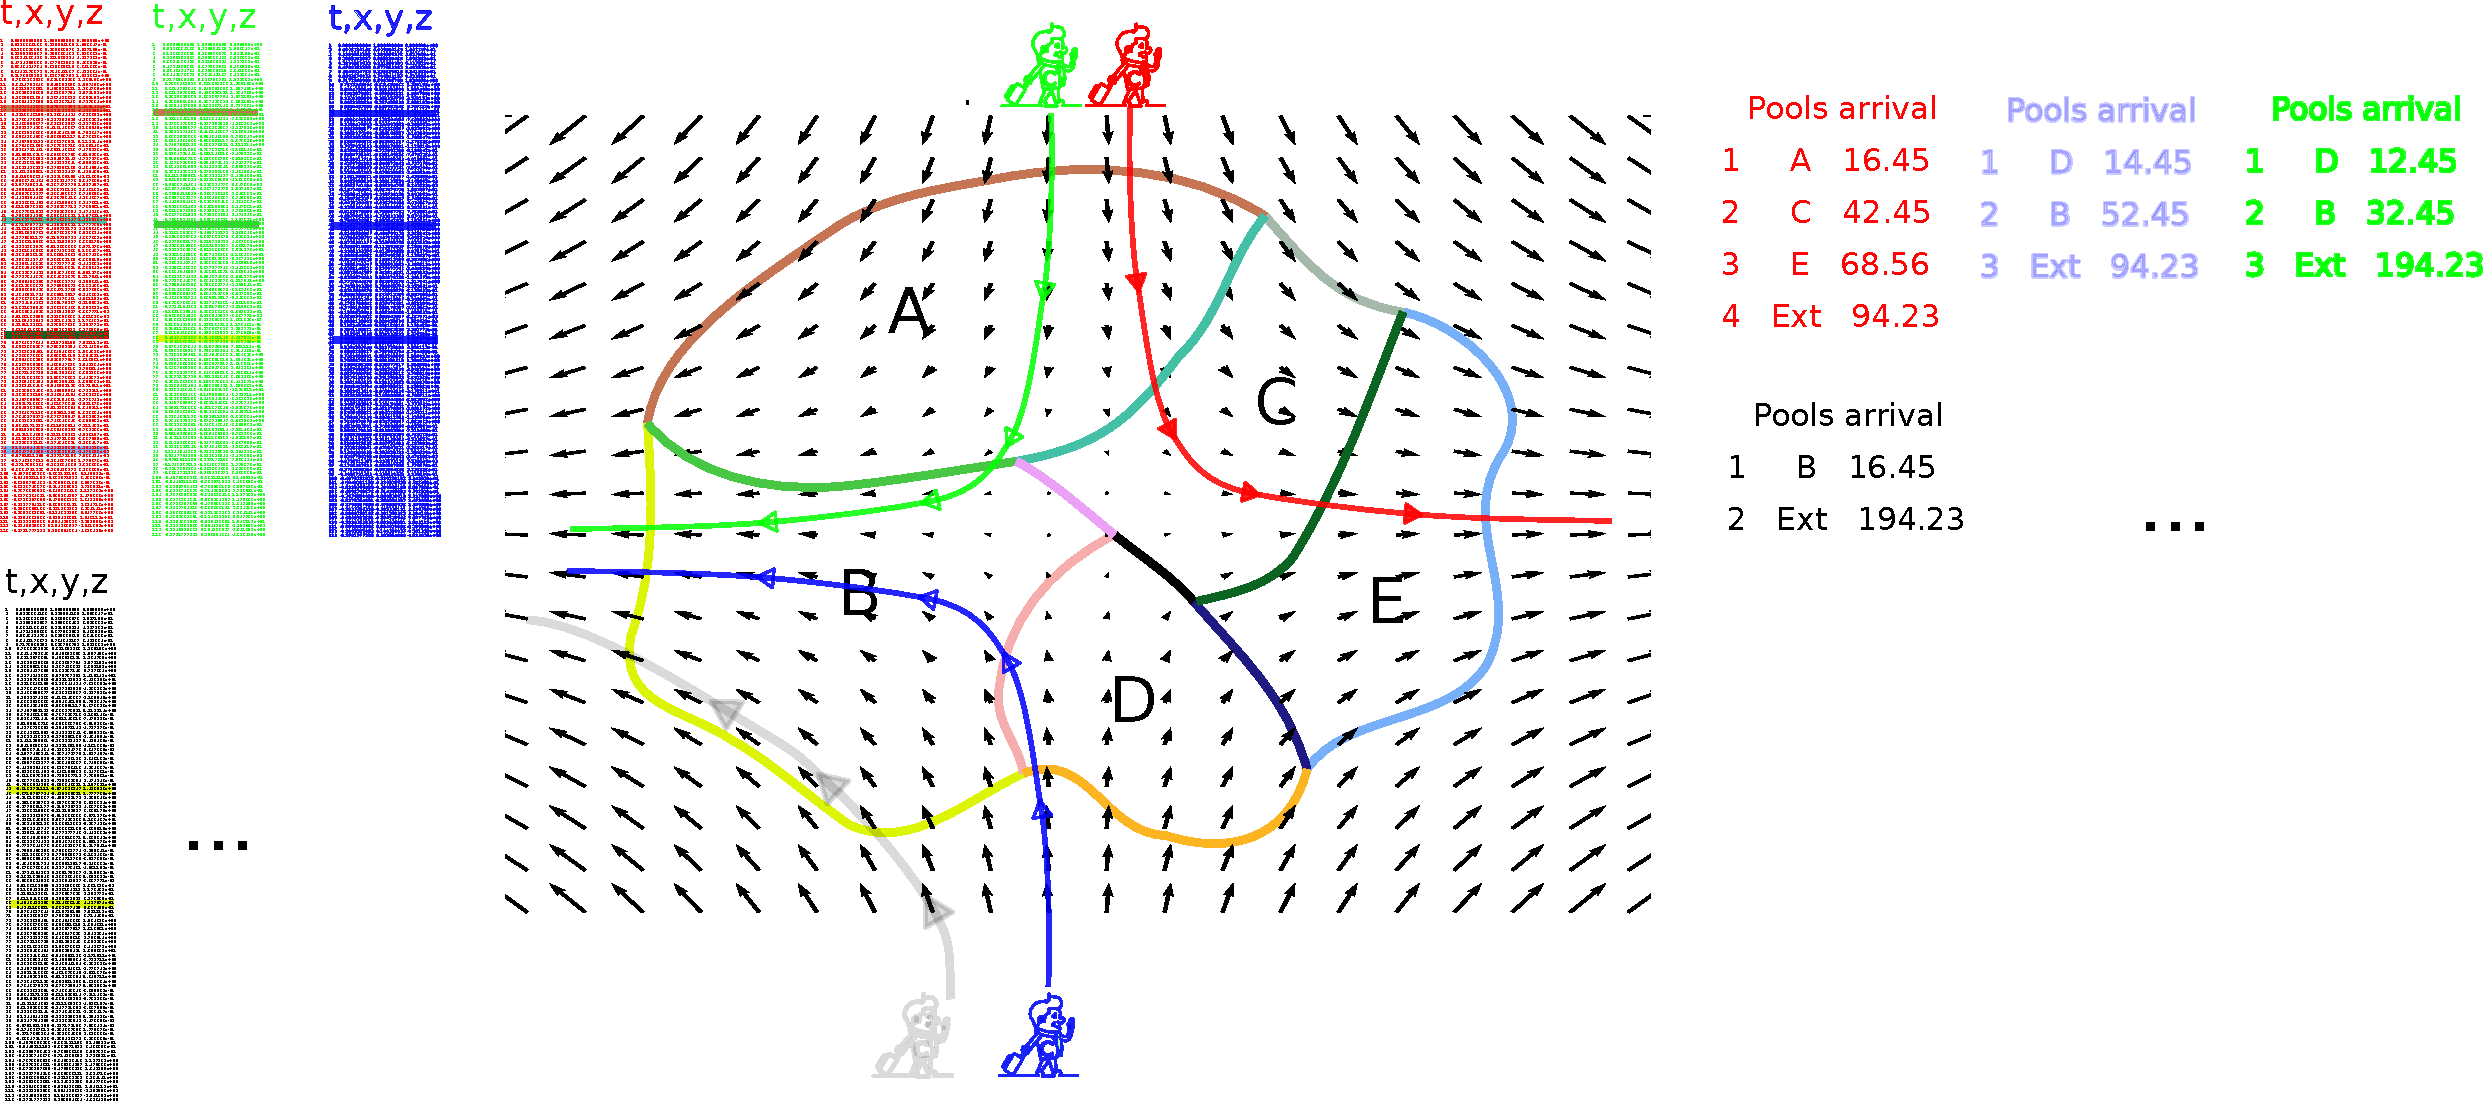
\includegraphics[width=0.99\textwidth]{VectorFieldWithOnePoolAndSubpoolsAndColoredBoundariesAndTrajectories.pdf} 
\end{frame}
%%%%%%%%%%%%%%%%%%%%%%%%%%%%%%%%%%%%%%%%%%%%%%%%%%%%%%%%%%%%%%%%%%%%%%%%%%%%%%%%%%%%%%%%%%%%%%%%%%%%%
\begin{frame}
	\frametitle{Possible  {\color{red} Descriptive} Statistics}
	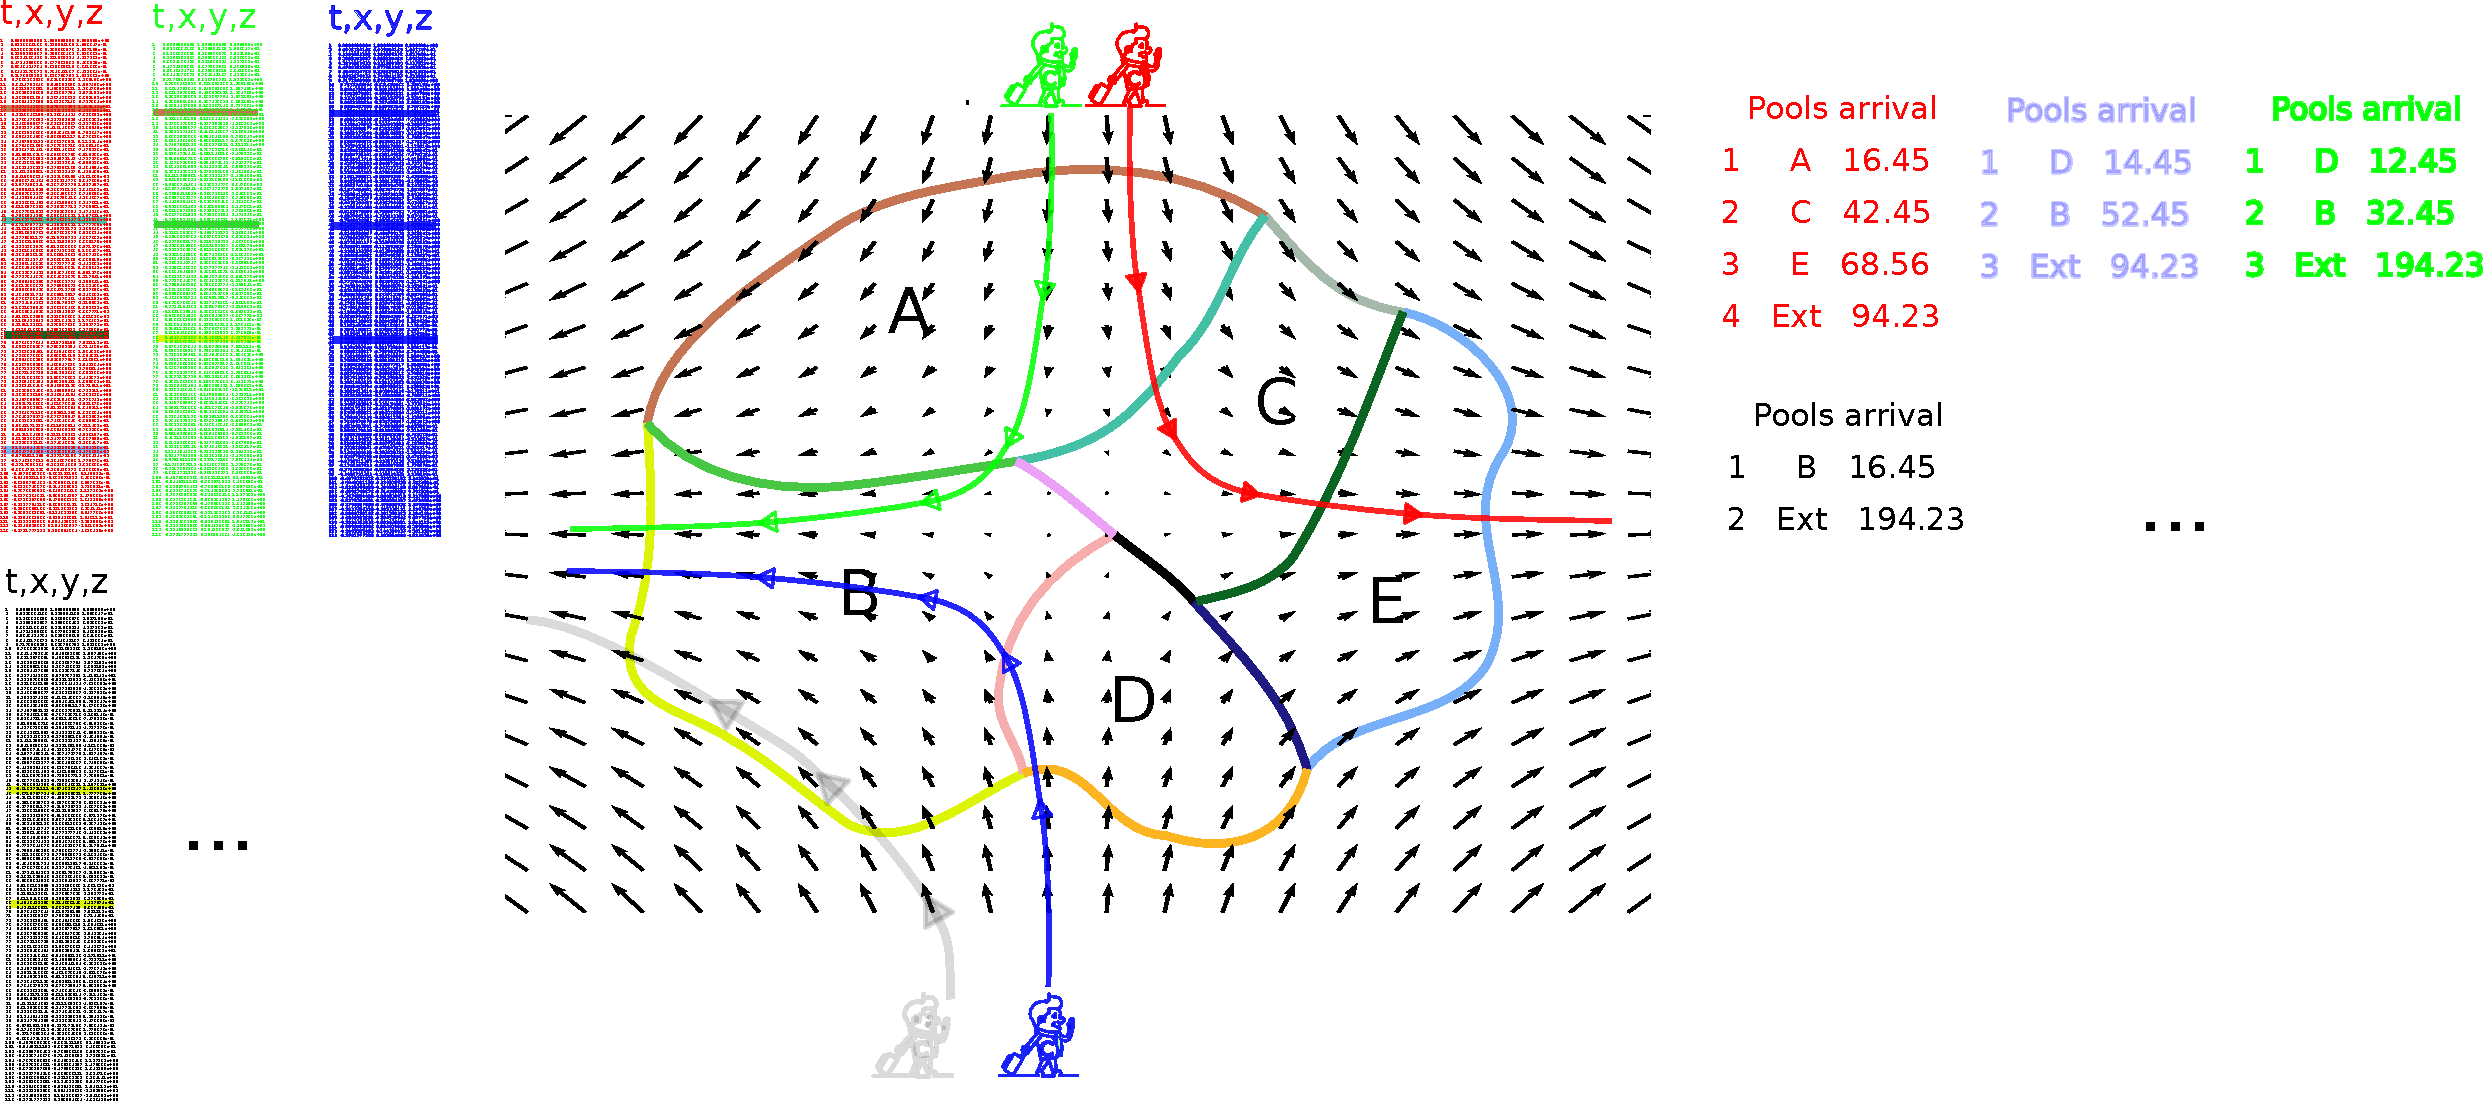
\includegraphics[height=0.45\textheight]{VectorFieldWithOnePoolAndSubpoolsAndColoredBoundariesAndTrajectories.pdf} 
	\begin{itemize}
		\item average time spent in a pool A ,B...
		\item average time spent in the whole system 
		\item average time of particles spent between pool C and E under the assumption of having entered by pool D (weird but possible...)
		\item number / mass of particles in pool A, B, 
		\item Deathrate of pool A.
		\item ...
	\end{itemize}
\end{frame}
%%%%%%%%%%%%%%%%%%%%%%%%%%%%%%%%%%%%%%%%%%%%%%%%%%%%%%%%%%%%%%%%%%%%%%%%%%%%%%%%%%%%%%%%%%%%%%%%%%%%%
\begin{frame}
\frametitle{Age of a Particle}
  \includegraphics<1,2,3>[width=0.6\textwidth]{ParticleAge.pdf}
  \note<1>{
  We can define the age of a particle with respect to the reservoir as the time it has spent in it.
  In the case of the human population this refers to the age in common sense.
  But in general the age refers not to the time of creation but to the time the reservoir was entered.
  If the reservoir in question is e.g. the soil and the particle a $^{14}C$ atom that entered the soil 5 minutes ago
  it is at least 
  possible that the atom is as old as the universe while its age with respect to the soil is only 5 minutes}
  
\begin{itemize}
     \item <2> The ``age '' is always defined in \emph{context} of the reservoir
     \item <3> The ``age '' can not be negative!
\end{itemize}

\end{frame}
%%%%%%%%%%%%%%%%%%%%%%%%%%%%%%%%%%%%%%%%%%%%%%%%%%%%%%%%%%%%%%%%%%%%%%%%%%%%%%%%%%%%%%%%%%%%%%%%%%%%%
\begin{frame}
 [fragile]
\frametitle{Mean Age }
\begin{itemize}
   \item Which set of particles to use for the average?\\ 
      proposition:
      \emph{all} particles that are in the reservoir at the given time. \\
      $\rightarrow$ usually depends on input rates as well as the dynamics of the system.
\end{itemize}
%\begin{tabular}{tt}
  \includegraphics<1>[height=0.3\textheight]{Reservoir_Peoples_Ages.pdf}
  \[
  \bar a(t) =\frac{a_1+a_2+\cdots+a_N}{N}
  \]
  With $N=N(t)$ the number of all particles in the reservoir at time $t$.
%\end{tabular}
  \note{To compute the average age of the population  of the world at a given time we would have to ask everybody how old he is and then compute the mean value.
  If we treat this room as a reservoir everybody would have started a stopwatch entering the room, press the stop button now and we would have to add all the times and divide them by the number of people.}
\end{frame}
%%%%%%%%%%%%%%%%%%%%%%%%%%%%%%%%%%%%%%%%%%%%%%%%%%%%%%%%%%%%%%%%%%%%%%%%%%%%%%%%%%%%%%%%%%%%%%%%%%%%%
\begin{frame}
 [fragile]
\frametitle{Mean Transit Time }
  \includegraphics<1>[height=0.3\textheight]{MeanTransitTime.pdf}
  \[
  \bar t_r(t) =\frac{a_1+a_2+\cdots+a_{n_{o}}}{n_{o}}
  \]
  With $n_{o}=n_{o}(t)$ the number of particles {\color{red} just leaving} at time $t$
\begin{itemize}
   \item Can be time dependent as well
      \pause
   \item Includes only the subset of particles that are just leaving at the given time.
   (Can only be computed when there is an output stream)
   %\item could be independent of input rates and only depend on the dynamics of the system.
\end{itemize}
\note{In the example of the world population it would be sufficient to observe the grave yards.
We would investigate the birth date of every person who dies and compute the average of the live spans. We ignore all the people still alive and concentrate only on the people just dying.
In this room it would be hard to compute the average transit time right now, because nobody is leaving at the moment. (dropping of to sleep does not count as leaving).
But we could after the talk.
Every person would press the stop bottom at its watch in the moment she passes the door.
If two or more people would leave in the same moment we could compute the average of the
times. 
It is also }
\end{frame}
%%%%%%%%%%%%%%%%%%%%%%%%%%%%%%%%%%%%%%%%%%%%%%%%%%%%%%%%%%%%%%%%%%%%%%%%%%%%%%%%%%%%%%%%%%%%%%%%%%%%%
\begin{frame}
 [fragile]
\frametitle{Differences between mean age and mean transit time}
\begin{tabular}{ll}
  \includegraphics<1>[height=0.2\textheight]{Reservoir_Peoples_Ages.pdf} 
  &
  \includegraphics<1>[height=0.2\textheight]{MeanTransitTime.pdf} 
  \\
  \parbox{0.45\textwidth}{
      \begin{itemize}
	 \item Includes { \color{red} all} particles that are in the reservoir at the given time.
         \item Directly coupled to input rates
      \end{itemize}
  }
  &
  \parbox{0.45\textwidth}{
      \begin{itemize}
	 \item Includes only the subset of particles that are {\color{red} just leaving} at the given time.
         \item Indirectly coupled to inputs 
      \end{itemize}
   }
\end{tabular}
\end{frame}
%%%%%%%%%%%%%%%%%%%%%%%%%%%%%%%%%%%%%%%%%%%%%%%%%%%%%%%%%%%%%%%%%%%%%%%%%%%%%%%%%%%%%%%%%%%%%%%%%%%%%
\begin{frame}
 [fragile]
\frametitle{Iteration over all particles}

   \begin{enumerate}
      \item
         To compute the mean transit time we have to identify the particles {\color{red} just leaving}.
      \item
         Ask every leaving  particle   when it entered and compute its age.
      \item
         Iterate over all particle and compute the average of their ages.
      \pause
     \[
     \bar t_r(t) =\frac{a_1+a_2+\cdots+a_{n_{o}}}{n_{o}}
     \]
     With $n_{o}=n_{o}(t)$ the number of particles just leaving at time $t$
   \end{enumerate}
\begin{knitrout}\footnotesize
\definecolor{shadecolor}{rgb}{0.969, 0.969, 0.969}\color{fgcolor}

{\centering 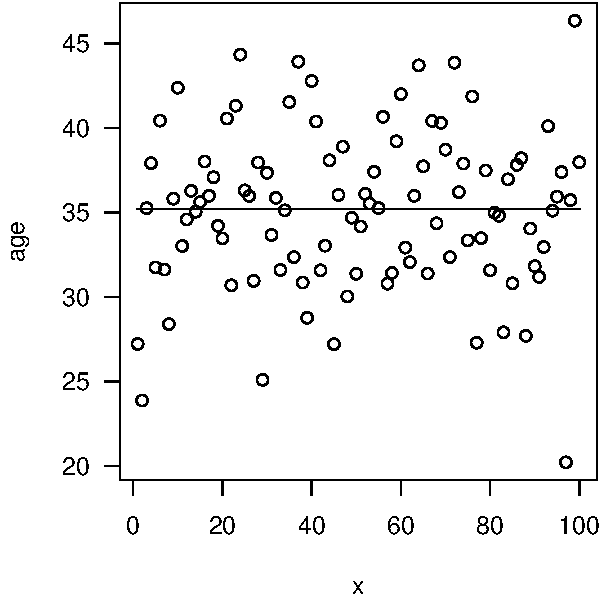
\includegraphics[width=.4\linewidth]{figure/beamer-mean-1} 

}



\end{knitrout}
\end{frame}
%%%%%%%%%%%%%%%%%%%%%%%%%%%%%%%%%%%%%%%%%%%%%%%%%%%%%%%%%%%%%%%%%%%%%%%%%%%%%%%%%%%%%%%%%%%%%%%%%%%%%%
\begin{frame}
 [fragile]
   \frametitle{Iteration over all {\color{red} ages}}
\begin{enumerate}
   \item as above
   \item as above + make a histogram of all ages
   \item iterate over all ages and compute their weighted average
      \pause
     \[
     \bar t_r(t) =\frac{a_1 n_{a_1} +a_2 n_{a_2} +\cdots+a_{n}n_{a_n}}{n_{o}}
     \]
     With $n_{o}=n_{o}(t)=n_{a_1} + n_{a_2} +\cdots +n_{a_n}$ 
   \end{enumerate}
\begin{knitrout}\footnotesize
\definecolor{shadecolor}{rgb}{0.969, 0.969, 0.969}\color{fgcolor}

{\centering 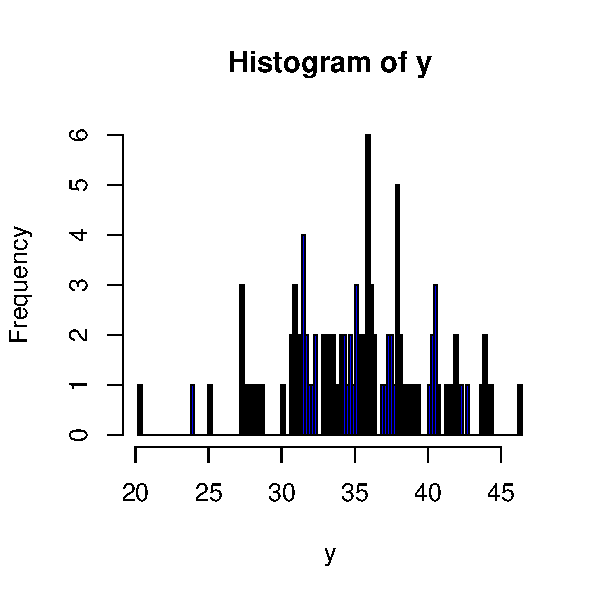
\includegraphics[width=.35\linewidth]{figure/beamer-histogram-1} 

}



\end{knitrout}
\end{frame}
%%%%%%%%%%%%%%%%%%%%%%%%%%%%%%%%%%%%%%%%%%%%%%%%%%%%%%%%%%%%%%%%%%%%%%%%%%%%%%%%%%%%%%%%%%%%%%%%%%%%%%
\begin{frame}
 [fragile]
   \frametitle{Integration over a {\color{red}density}}
\begin{eqnarray*}
     \bar t_r(t) &=&\lim_{n\to \infty} \frac{a_1 n_{a_1} +a_2 n_{a_2} +\cdots+a_{n}n_{a_n}}{n_{o}}
     \\
     &=&\lim_{n\to \infty}\sum_{minage}^{maxage} a \frac{n(a)}{n_o} da
     \\
     &=&\int_{minage}^{maxage} a \psi(a) da
\end{eqnarray*}
\begin{knitrout}\footnotesize
\definecolor{shadecolor}{rgb}{0.969, 0.969, 0.969}\color{fgcolor}

{\centering 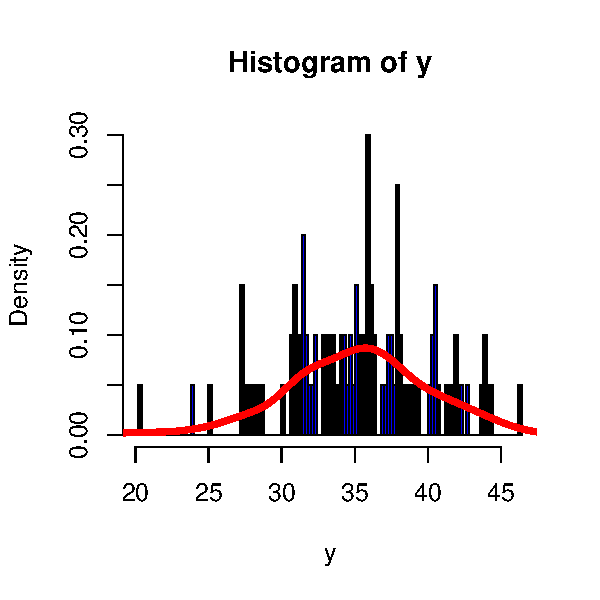
\includegraphics[width=.35\linewidth]{figure/beamer-dens-1} 

}



\end{knitrout}
\end{frame}
%%%%%%%%%%%%%%%%%%%%%%%%%%%%%%%%%%%%%%%%%%%%%%%%%%%%%%%%%%%%%%%%%%%%%%%%%%%%%%%%%%%%%%%%%%%%%%%%%%%%%%
\begin{frame}
 [fragile]
 \frametitle{Same procedure for {\color{red} age} density}
\begin{eqnarray*}
     \bar a(t) &=&\lim_{n\to \infty} \frac{a_1 n_{a_1} +a_2 n_{a_2} +\cdots+a_{n}n_{a_n}}{n_{p}}
     \\
     &=&\lim_{n\to \infty}\sum_{minage}^{maxage} a \frac{n(a)}{n_p} da
     \\
     &=&\int_{minage}^{maxage} a \phi(a) da
\end{eqnarray*}
\begin{knitrout}\footnotesize
\definecolor{shadecolor}{rgb}{0.969, 0.969, 0.969}\color{fgcolor}

{\centering 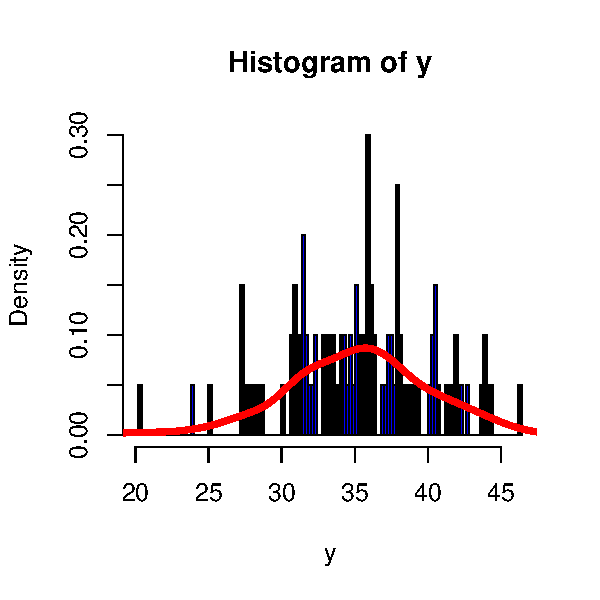
\includegraphics[width=.35\linewidth]{figure/beamer-dens2-1} 

}
\end{knitrout}
\end{frame}
%%%%%%%%%%%%%%%%%%%%%%%%%%%%%%%%%%%%%%%%%%%%%%%%%%%%%%%%%%%%%%%%%%%%%%%%%%%%%%%%%%%%%%%%%%%%%%%%%%%%%
\subsection{Answer Questions more simply}
%%%%%%%%%%%%%%%%%%%%%%%%%%%%%%%%%%%%%%%%%%%%%%%%%%%%%%%%%%%%%%%%%%%%%%%%%%%%%%%%%%%%%%%%%%%%%%%%%%%%%
\begin{frame}
	\frametitle{Possible {\color{red} Predictive} Statistics ?}
	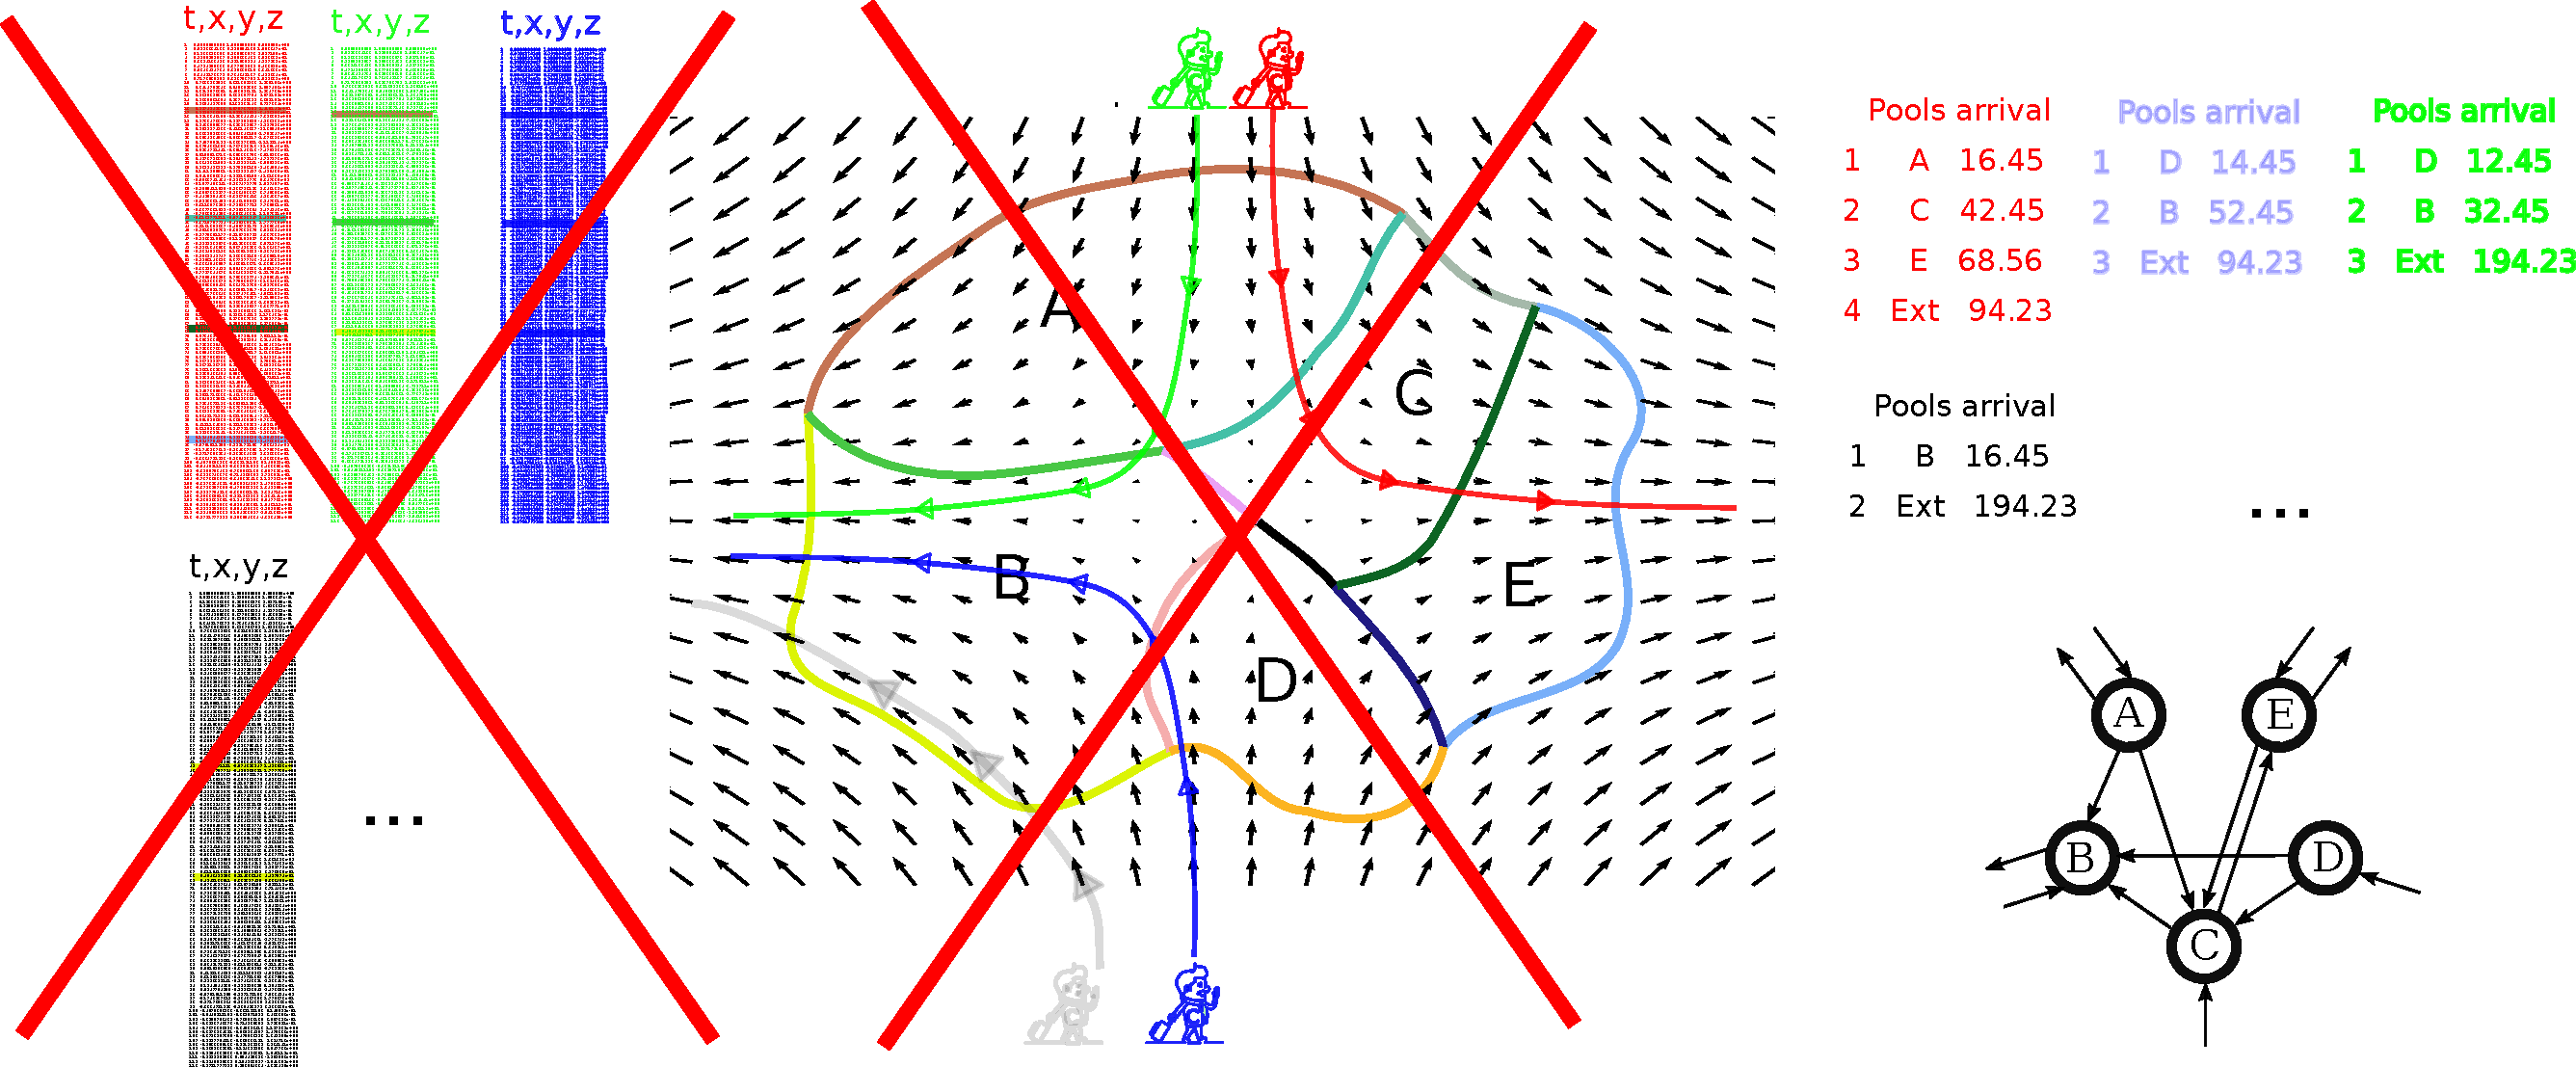
\includegraphics[height=0.45\textheight]{VectorFieldWithOnePoolAndSubpoolsAndColoredBoundariesAndCrossedTrajectories.pdf} 
	\begin{itemize}
	\item
		Could we make a rule to predict the number of particles exiting from Pool E at time using only the particle passports? (Assuming that the exit from E is not recorded.)  
	\item
		Could we make a rule to predict the age distribution of particles exiting from Pool E at time using only the particle passports? (Assuming again that the exit from E is not recorded.)  

	\end{itemize}
\end{frame}
%\begin{frame}
% [fragile]
%\frametitle{Example Model}
%\makebox[0pt][l]{
%  \includegraphics<1>[width=0.9\textwidth]{LasagaModel.pdf}
%  \includegraphics<2,3,4,5,6,7,8>[width=0.9\textwidth]{LasagaModelTransp.pdf}
%  }
%\raisebox{4cm}{
%\begin{minipage}{10cm}
%   \begin{itemize}
%      \item<2,3,4,5,6,7,8>
%	 We want to observe the behavior of arbitrary complex reservoir systems 
%	 under all imaginable conditions,which e.g. means:\\
%	 %\begin{itemize}
%	    \item<3,4,5,6,7,8>
%	       time dependent transfer rates.
%	    \item<4,5,6,7,8>
%	       time dependent inputs
%	    \item <5,6,7,8>
%	       non linear behavior
%	    \item<6,7,8>
%	       arbitrary perturbations (non steady states)
%	    \item<7,8>
%	       closed and open systems
%	    \item<8>
%	       reservoirs with nested reservoirs
%	 %\end{itemize}
%   \end{itemize}
%\end{minipage}
%}
%  \note{
%  We want to observe the behavior of arbitrary complex reservoir systems 
%  under all imaginable conditions. \\
%  To raise your interest we have chosen an example of an old global Carbon cycle model, that 
%  has some of the features we are interested in.}
%\end{frame}
%%%%%%%%%%%%%%%%%%%%%%%%%%%%%%%%%%%%%%%%%%%%%%%%%%%%%%%%%%%%%%%%%%%%%%%%%%%%%%%%%%%%%%%%%%%%%%%%%%%%%
%\begin{frame}
% [fragile]
%\frametitle{inappropriateness of previously proposed analytical solutions}
%\begin{itemize}
%      \pause
%      \item
%	 Only available for special cases 
%      \pause
%      \item
%	 involve a lot of assumptions that can be confusing sometimes, e.g.:
%      \pause
%      \begin{itemize}
%	    \item
%	    steady states, 
%      \pause
%	    \item
%	    time invariant systems
%      \pause
%	    \item
%	    linear systems 
%      \pause
%	    \item
%	    impulsive or constant inputs 
%      \pause
%      \end{itemize}
%      \pause
%      \item
%	 assumptions sometimes hard to recognize 
%	 \\
%      \pause
%	 $\rightarrow$ misleading into wrong generalizations
%	 \\
%      \pause
%	 $\rightarrow$ motivation for a numerical counterpart 
%	 where all the assumptions (if any) should be 
%	 {\color{red} intuitive and obvious.}
%\end{itemize}
%\end{frame}
%%%%%%%%%%%%%%%%%%%%%%%%%%%%%%%%%%%%%%%%%%%%%%%%%%%%%%%%%%%%%%%%%%%%%%%%%%%%%%%%%%%%%%%%%%%%%%%%%%%%%%
%\section{Our proposed solution}
%\subsection{Definitions}
%
%%%%%%%%%%%%%%%%%%%%%%%%%%%%%%%%%%%%%%%%%%%%%%%%%%%%%%%%%%%%%%%%%%%%%%%%%%%%%%%%%%%%%%%%%%%%%%%%%%%%%%
%\begin{frame}
% [fragile]
%\frametitle{Requirements for definitions}
%definitions should be:
%\begin{enumerate}
%      \pause
%   \item as generally applicable as possible\\
%      $\rightarrow$ observable even in the real world
%      \pause
%   \item easy to check
%      \pause
%   \item suitable for computer simulations \\
%      \pause
%      $\rightarrow$ based on a definite time scale with
%      \begin{enumerate}
%	 \item definite start
%	 \item definite end \\
%      \pause
%	 $\rightarrow$ no $\infty$
%      \end{enumerate}
%\end{enumerate}
%\note{
%Assume that we want to run a particle simulation, that we want to ``observe'' So all features used should be observable in the real world too.
%To formulate the problem in a numerical way we need to define the basic concepts precisely and in a way that a computer would understand. This means that we should avoid infinities.
%While the definitions are clear in some cases, there are subtle differences in details that may change the interpretations considerably.}
%\end{frame}
%%%%%%%%%%%%%%%%%%%%%%%%%%%%%%%%%%%%%%%%%%%%%%%%%%%%%%%%%%%%%%%%%%%%%%%%%%%%%%%%%%%%%%%%%%%%%%%%%%%%%%%
%\begin{frame}
%\frametitle{The general concept of a reservoir}
%  %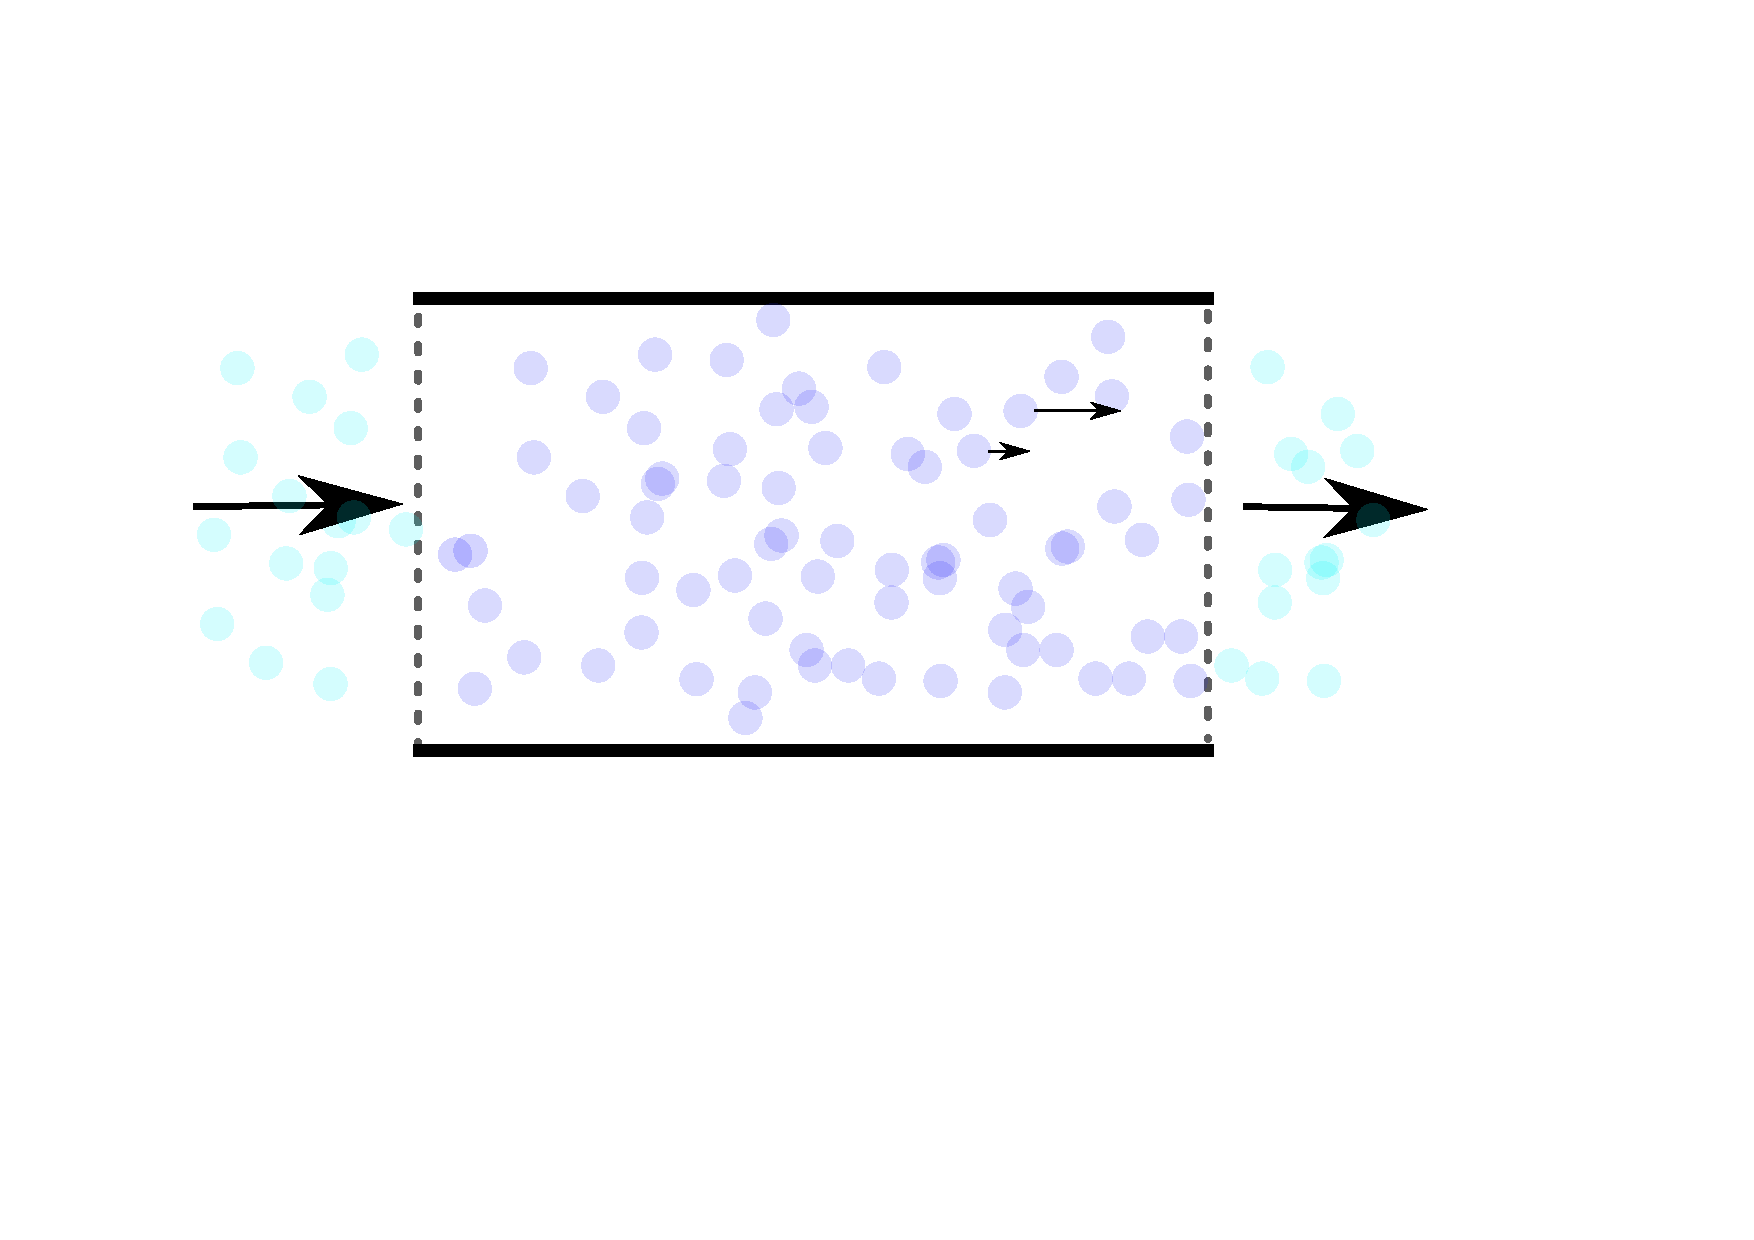
\includegraphics[height=0.8\textheight]{Reservoir.pdf}
%  \includegraphics<1>[height=0.5\textheight]{Reservoir.pdf}
%  %\includegraphics<2>[height=0.5\textheight]{Reservoir_People.pdf}
%  \includegraphics<3,4>[height=0.5\textheight]{ReservoirNested.pdf} 
%  \begin{enumerate}
%\item <1,2,3,4> 
%   In and out ``flows'' must be unambiguously  defined \\
%\item <2,3,4> 
%   ``Flows'' do not necessarily involve ``movement'' \\
%     In and out flow ``channels'' do not always have to be defined physically or spatially 
%\item <3,4> 
%   reservoirs can have arbitrary complex subsctructures
%\item <4> 
%   reservoirs can be mixed or not
%\end{enumerate}
%\note<1>{Imagine a reservoir of particles with an input and an output channel. 
%Particles will enter the system through some input channel, will stay there for a while and eventually leave the system through an output stream. 
%Here Only the dark blue particles are ``in'' the reservoir. 
%}
%\note<2>{
%Although the concept of a reservoir is usually intuitively attached to some kind of a pool with fluid moving trough it 
%the idea is more general. 
%
%An example that shows how generally this idea can be applied is the human population of the world.
%A particle here refers to a human being that is born, lives and dies.
%
%The inflow and outflow boundaries are not spatially defined in this case 
%}
%
%\end{frame}
%%%%%%%%%%%%%%%%%%%%%%%%%%%%%%%%%%%%%%%%%%%%%%%%%%%%%%%%%%%%%%%%%%%%%%%%%%%%%%%%%%%%%%%%%%%%%%%%%%%%%%
%\begin{frame}
%      \pause
%\begin{enumerate}
%   \item describe the rate of change for the stuff inside the system in the form inputrate - outputrate
%      which is possible for all reservoir systems:
%      $\dot{C}=F(C,t)=I(C,t)-O(C,t)$
%      \pause
%   \item solve the possibly nonlinear system (compute $C(t)$)
%      \pause
%   \item use the solution to transform it to a linear uncoupled system with {\color{red} exactly } the same solution
%      \pause
%   \item for every $t$ and every $a:0<a<t$ compute $\psi(a,t)$
%      \pause
%   \item for every $t$ 
%   	 compute the expected value of $a$ by integrating over the product:
%	 \[ 
%	 E(t)=\int_0^t \psi(a,t) \;a \; da
%	 \]
%\end{enumerate}
%\end{frame}
%%%%%%%%%%%%%%%%%%%%%%%%%%%%%%%%%%%%%%%%%%%%%%%%%%%%%%%%%%%%%%%%%%%%%%%%%%%%%%%%%%%%%%%%%%%%%%%%%%%%%%
%\begin{frame}
% [fragile]
%\frametitle{Transforming the system I}
%  inject the solution into the operator
%      \begin{eqnarray*}
%	 \dot{\vec{F}}	&=&\dot{\vec{C}}(\vec{C},t)\\
%	 &=&
%	 \left(
%	 \begin{array}{c}
%	    \dot{F}_1(C_1,\hdots ,C_n,t)\\
%	    \vdots \\
%	    \dot{F}_n(C_1,\hdots ,C_n,t)
%	 \end{array}
%	 \right)
%	 \\
%	 &=&
%	 \left(
%	 \begin{array}{c}
%	    \dot{I}_1(C_1,\hdots ,C_n,t)\\
%	    \vdots \\
%	    \dot{I}_n(C_1,\hdots ,C_n,t)
%	 \end{array}
%	 \right)
%	 +
%	 \left(
%	 \begin{array}{c}
%	    \dot{O}_1(C_1,\hdots ,C_n,t)\\
%	    \vdots \\
%	    \dot{O}_n(C_1,\hdots ,C_n,t)
%	 \end{array}
%	 \right)
%      \end{eqnarray*}
%\end{frame}
%%%%%%%%%%%%%%%%%%%%%%%%%%%%%%%%%%%%%%%%%%%%%%%%%%%%%%%%%%%%%%%%%%%%%%%%%%%%%%%%%%%%%%%%%%%%%%%%%%%%%%
%\begin{frame}
% [fragile]
%\frametitle{Transforming the system II}
%  For every component $F_i$ do:    
%      \begin{eqnarray*}
%	 \dot{F}_i(t) &=&\frac{I_i(C_1(t),\hdots ,C_n(t),t)}{C_i(t)}C_i(t)-\frac{O_i(C_1(t),\hdots ,C_n(t),t)}{C_i(t)}C_i(t)\\
%	 &=&I_{i_{lin}}(t)C_i(t)-O_{i_{lin}}(t)C_i(t)\\
%	 &=&F_{i_{lin}}(t)C_i(t)
%      \end{eqnarray*}
%  Now the equations are uncoupled and linear.    
%%      for all times ${\color{red}t}$ for which the result is sought compute $\bar{a}({\color{red}t})$ as follows: (the next slide has to be evaluated many times)
%\end{frame}
%%%%%%%%%%%%%%%%%%%%%%%%%%%%%%%%%%%%%%%%%%%%%%%%%%%%%%%%%%%%%%%%%%%%%%%%%%%%%%%%%%%%%%%%%%%%%%%%%%%%%%%
%\begin{frame}
% [fragile]
%\frametitle{Accumulating previous inputs}
%\begin{knitrout}\footnotesize
%\definecolor{shadecolor}{rgb}{0.969, 0.969, 0.969}\color{fgcolor}
%
%{\centering 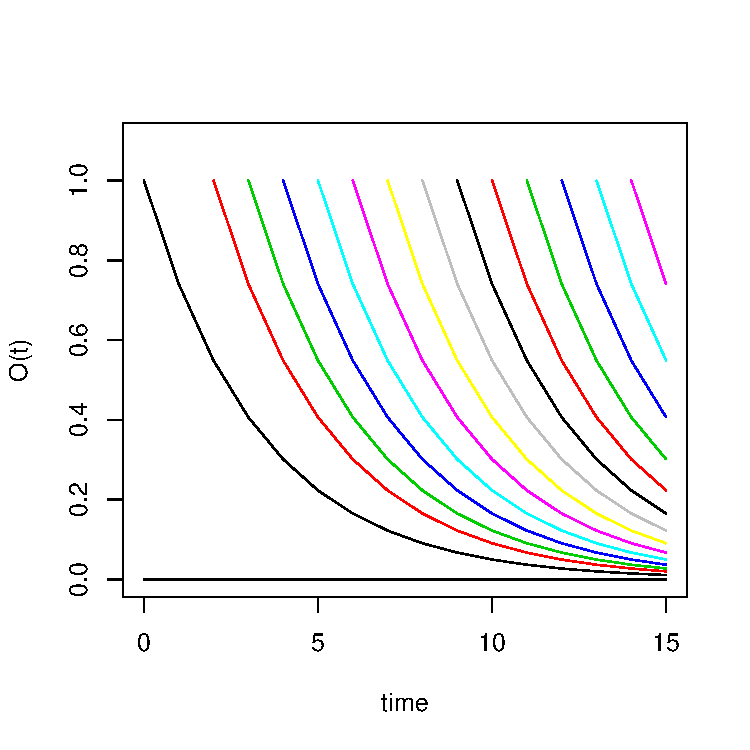
\includegraphics[width=.7\linewidth]{figure/beamer-O12-1} 
%
%}
%
%
%
%\end{knitrout}
%\end{frame}
%%%%%%%%%%%%%%%%%%%%%%%%%%%%%%%%%%%%%%%%%%%%%%%%%%%%%%%%%%%%%%%%%%%%%%%%%%%%%%%%%%%%%%%%%%%%%%%%%%%%%%%
%\begin{frame}
% [fragile]
% \frametitle{Compute $\psi( {\color{green}a}, {\color{red}t})$ }
% for every possible age $0<{\color{green}a}<{\color{red}t}$ (nested loop) compute the probability density
% $\psi(
% {\color{green}a},
% {\color{red}t}
% )$ 
% as follows:
%   	 \begin{enumerate}
%      \pause
%   	    \item
%   	       collect all inputs that have occurred since $t-a$   
%      \pause
%   	    \item 
%	       predict their time development (vanishing) under no input conditions (solve for $O_{lin}$)
%      \pause
%   	    \item 
%   	       integrate over all those partly vanished inputs to find out what is left of
%   	       the lot
%      \pause
%   	    \item 
%   	       divide by the amount of stuff present in the reservoir right now to get the probability for a particle 
%   	       to have age less than a and be still around.
%      \pause
%	    \item
%	       compute the derivative with respect to $a$ 
%   	 \end{enumerate}
%\end{frame}
%
%%%%%%%%%%%%%%%%%%%%%%%%%%%%%%%%%%%%%%%%%%%%%%%%%%%%%%%%%%%%%%%%%%%%%%%%%%%%%%%%%%%%%%%%%%%%%%%%%%%%%%
%\subsection{Comparison to standard theory}
%%%%%%%%%%%%%%%%%%%%%%%%%%%%%%%%%%%%%%%%%%%%%%%%%%%%%%%%%%%%%%%%%%%%%%%%%%%%%%%%%%%%%%%%%%%%%%%%%%%%%%
%\begin{frame}
% [fragile]
%\frametitle{Conceptual example}
%\begin{itemize}
%   \item Input(rate): impulsive only at the start $\dot{I}=C_0\delta(0)$
%   \item Output(rate): $\dot{O}(C,t)=-k C(t)$ 
%   \item wanted: $C(t),\phi(t),\psi(t),\bar{t_r},\bar{a}$
%      \pause
%   \item solution:
%   \begin{itemize}
%      \pause
%      \item 
%	 $C(t)=C_0 e^{-k t}$   
%\begin{knitrout}\footnotesize
%\definecolor{shadecolor}{rgb}{0.969, 0.969, 0.969}\color{fgcolor}
%
%{\centering 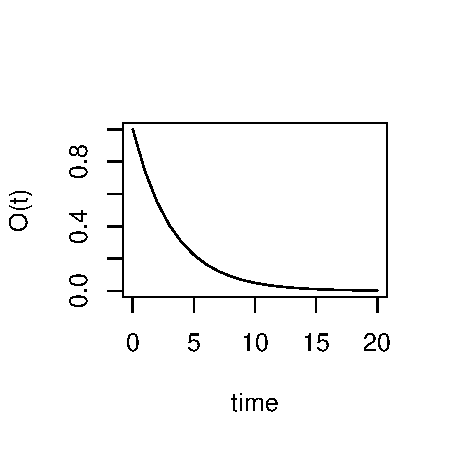
\includegraphics[width=.6\linewidth]{figure/beamer-O-1} 
%
%}
%
%
%
%\end{knitrout}
%      \end{itemize}
%   \end{itemize}
%\end{frame}
%%%%%%%%%%%%%%%%%%%%%%%%%%%%%%%%%%%%%%%%%%%%%%%%%%%%%%%%%%%%%%%%%%%%%%%%%%%%%%%%%%%%%%%%%%%%%%%%%%%%%%
%\begin{frame}
% [fragile]
%\frametitle{Intuitive solution for the example}
%   \includegraphics<1>[width=\textwidth]{MeanAgeImpuls.pdf}
%\end{frame}
%%%%%%%%%%%%%%%%%%%%%%%%%%%%%%%%%%%%%%%%%%%%%%%%%%%%%%%%%%%%%%%%%%%%%%%%%%%%%%%%%%%%%%%%%%%%%%%%%%%%%%%
%\begin{frame}
%[fragile]
%\frametitle{Theory for the example}
%      Manzoni,Katul,Porporato 2009:\\
%      ``for any linear systems  the transit time
%      distribution is the output flow resulting from an impulsive
%      unitary input.''
%   \begin{eqnarray*}
%      O(t)&=&\int_{0}^{\infty} \psi(T)I(t-T)dT
%	 \\
%	 &=&\psi(t) \text{ for } I=\delta(t-T)
%	 \\
%	 &=& e^{-kt} 
%   \end{eqnarray*}
%      \pause
%   Additionally we have:\\
%      $\phi(a)=\psi(a)=e^{-k a},\bar{t_r}=\bar{a}=\frac{1}{k}$
%   \\
%   Questions:
%	 \pause
%   \begin{itemize}
%      \item Where does the $\infty$ come from?
%	 \pause
%      \item is $\phi(a)=\psi(a)=e^{-k a}$ a probability density if we start the whole thing at some 
%	 definite time and not infinitely long ago? \\
%	 (does it integrate to $1$ ?)
%	 \pause
%      \item Are the above densities valid for arbitrary inputrates  $I(t)$ 
%	 \\
%	 (as functions of time.) 
%	 \pause
%	 \note{may be forever}
%   \end{itemize}
%\end{frame}
%%%%%%%%%%%%%%%%%%%%%%%%%%%%%%%%%%%%%%%%%%%%%%%%%%%%%%%%%%%%%%%%%%%%%%%%%%%%%%%%%%%%%%%%%%%%%%%%%%%%%%%
%\begin{frame}
% [fragile]
%\frametitle{Intuitive Solution to the Example}
%   \includegraphics<1>[width=\textwidth]{MeanAgeImpuls.pdf}
%\end{frame}
%%%%%%%%%%%%%%%%%%%%%%%%%%%%%%%%%%%%%%%%%%%%%%%%%%%%%%%%%%%%%%%%%%%%%%%%%%%%%%%%%%%%%%%%%%%%%%%%%%%%%%
%\begin{frame}
% [fragile]
%\frametitle{Conceptual example II}
%\begin{itemize}
%   \item Input(rate): constant $I_0=C_0 k$
%   \item Output(rate): $\dot{O}(C,t)=-k C(t)$ 
%   \item wanted: $C(t),\phi(t),\psi(t),\bar{t_r},\bar{a}$
%      \pause
%   \item solution:
%   \begin{itemize}
%      \item 
%	 $C(t)=C_0$
%\begin{knitrout}\footnotesize
%\definecolor{shadecolor}{rgb}{0.969, 0.969, 0.969}\color{fgcolor}
%
%{\centering 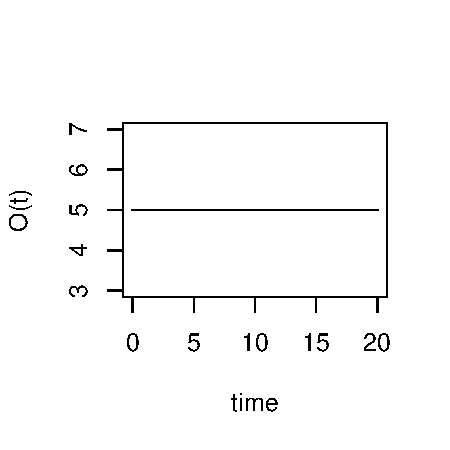
\includegraphics[width=.6\linewidth]{figure/beamer-OII-1} 
%
%}
%
%
%
%\end{knitrout}
%      \end{itemize}
%   \end{itemize}
%\end{frame}
%%%%%%%%%%%%%%%%%%%%%%%%%%%%%%%%%%%
%\begin{frame}
% [fragile]
%\frametitle{Intuitive Solution to the Example in steady state}
%   \includegraphics<1>[width=\textwidth]{MeanAgeSteady.pdf}
%\end{frame}
%%%%%%%%%%%%%%%%%%%%%%%%%%%%%%%%%%%%%%%%%%%%%%%%%%%%%%%%%%%%%%%%%%%%%%%%%%%%%%%%%%%%%%%%%%%%%%%%%%%%%%
%%\begin{frame}
%%\frametitle{Confusing Definitions}
%%\begin{tabular}{|c|c|c|}
%%\hline
%%Source &   Name 	& Definition \\
%%\hline
%%%Example text outside R code here; we know the value of pi is pi.
%%\end{tabular}
%%\end{frame}
%%%%%%%%%%%%%%%%%%%%%%%%%%%%%%%%%%%%%%%%%%%%%%%%%%%%%%%%%%%%%%%%%%%%%%%%%%%%%%%%%%%%%%%%%%%%%%%%%%%%%%
%%
%%%%%%%%%%%%%%%%%%%%%%%%%%%%%%%%%%%%%%%%%%%%%%%%%%%%%%%%%%%%%%%%%%%%%%%%%%%%%%%%%%%%%%%%%%%%%%%%%%%%%
%\section{Example}
%\begin{frame}
% [fragile]
%\frametitle{Example Model}
%  \includegraphics<1>[width=0.9\textwidth]{LasagaModel.pdf}
%\end{frame}
%%%%%%%%%%%%%%%%%%%%%%%%%%%%%%%%%%%%%%%%%%%%%%%%%%%%%%%%%%%%%%%%%%%%%%%%%%%%%%%%%%%%%%%%%%%%%%%%%%%%
%\begin{frame}
% [fragile]
%\frametitle{Didactical Considerations}
%
%\makebox[0pt][l]{
%  \includegraphics<1>[width=0.9\textwidth]{LasagaModelTransp.pdf}
%  \includegraphics<2>[width=0.9\textwidth]{LasagaModelTranspEquation.pdf}
%  \includegraphics<3>[width=0.9\textwidth]{LasagaModelTranspEquationLast.pdf}
%  \includegraphics<4>[width=0.9\textwidth]{LasagaModelTranspEquationLastWithParts.pdf}
%  \includegraphics<5>[width=0.9\textwidth]{LasagaModelTranspEquationLastWithPartsImputOutput.pdf}
%}
%\raisebox{5cm}{
%\begin{minipage}{10cm}
%   \begin{itemize}
%      \item<1,2,3>
%      The system is a \emph{cycle}. \\ 
%      $\rightarrow$ Nothing leaves the system as a whole. \\
%      $\rightarrow$ Transit times for the whole system do not make sense.\\
%      $\rightarrow$ We will observe sub reservoirs \\
%      \item<2,3> 
%	 We want to demonstrate a use case not accessible with analytic methods. \\
%	 $\rightarrow$ we will perturb the system out of its steady state.
%	 Fortunately \emph{all} equations are nonlinear. So there is no chance to
%	 compute anything without a numerical method.
%      \item <3> We do not want to complicate matters unnecessarily.\\
%      $\rightarrow$ We will go for the simplest equation.\\
%      $\rightarrow$ observe the last pool.\\
%   \end{itemize}
%\end{minipage}
%}
%\end{frame}
%%%%%%%%%%%%%%%%%%%%%%%%%%%%%%%%%%%%%%%%%%%%%%%%%%%%%%%%%%%%%%%%%%%%%%%%%%%%%%%%%%%%%%%%%%%%%%%%%%%%%%%
%\subsection{Results}
%%%%%%%%%%%%%%%%%%%%%%%%%%%%%%%%%%%%%%%%%%%%%%%%%%%%%%%%%%%%%%%%%%%%%%%%%%%%%%%%%%%%%%%%%%%%%%%%%%%%%%%
%%\begin{frame}
%%[fragile]
%%\frametitle{Python}
%%Now we proudly present a python script that uses sympy to produce the latex part.
%%<<mm,echo=FALSE,eval=TRUE,engine='python',results="asis">>=
%%from meanage import *
%%lp(dic["sol_abstract"])
%%lp(dic["sol_constant"])
%%@
%%\end{frame}
%%%%%%%%%%%%%%%%%%%%%%%%%%%%%%%%%%%%%%%%%%%%%%%%%%%%%%%%%%%%%%%%%%%%%%%%%%%%%%%%%%%%%%%%%%%%%%%%%%%%%%
%\begin{frame}
% [fragile]
%\frametitle{Solution}
%  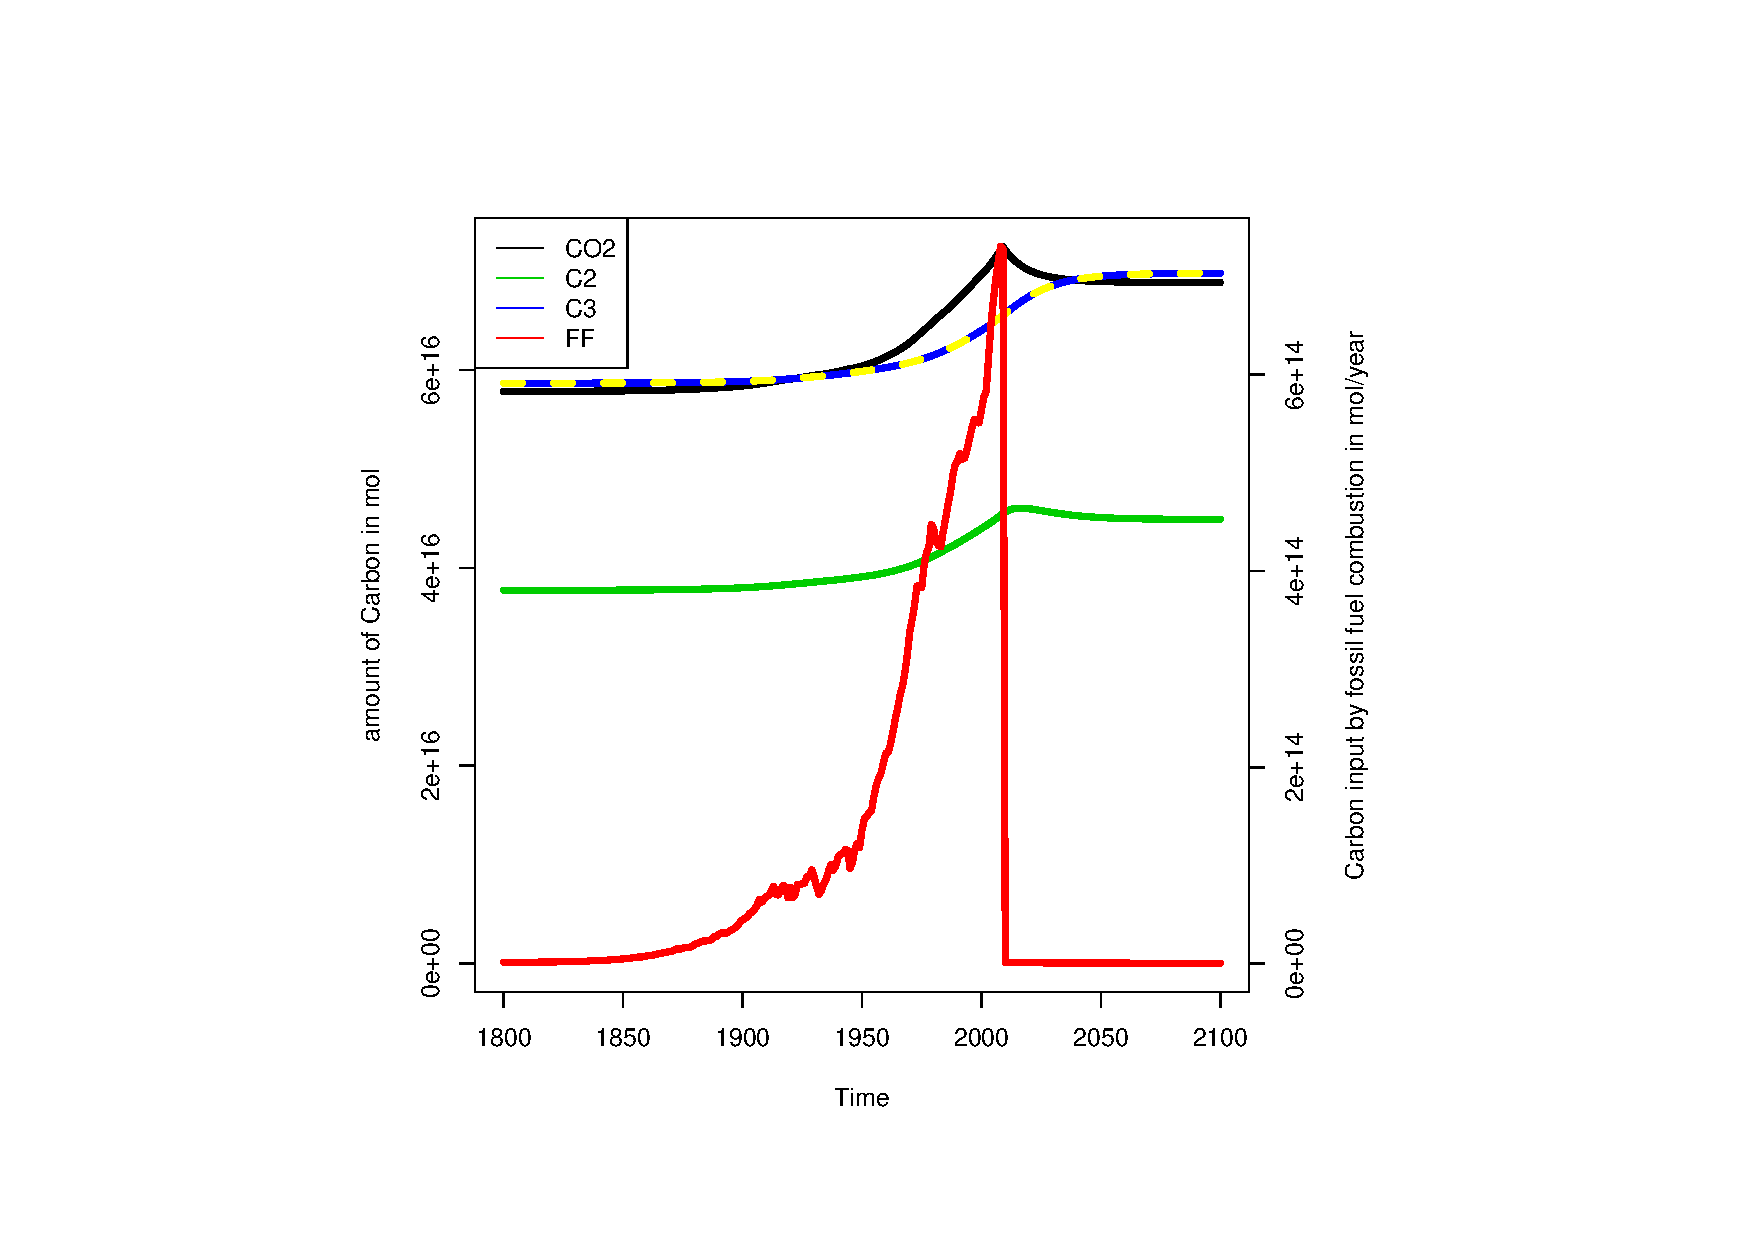
\includegraphics[width=0.9\textwidth]{NonlinearAtmosphericModelLong.pdf}
%\end{frame}
%%%%%%%%%%%%%%%%%%%%%%%%%%%%%%%%%%%%%%%%%%%%%%%%%%%%%%%%%%%%%%%%%%%%%%%%%%%%%%%%%%%%%%%%%%%%%%%%%%%%%%
%\begin{frame}
% [fragile]
%\frametitle{Mean age as function of time}
%  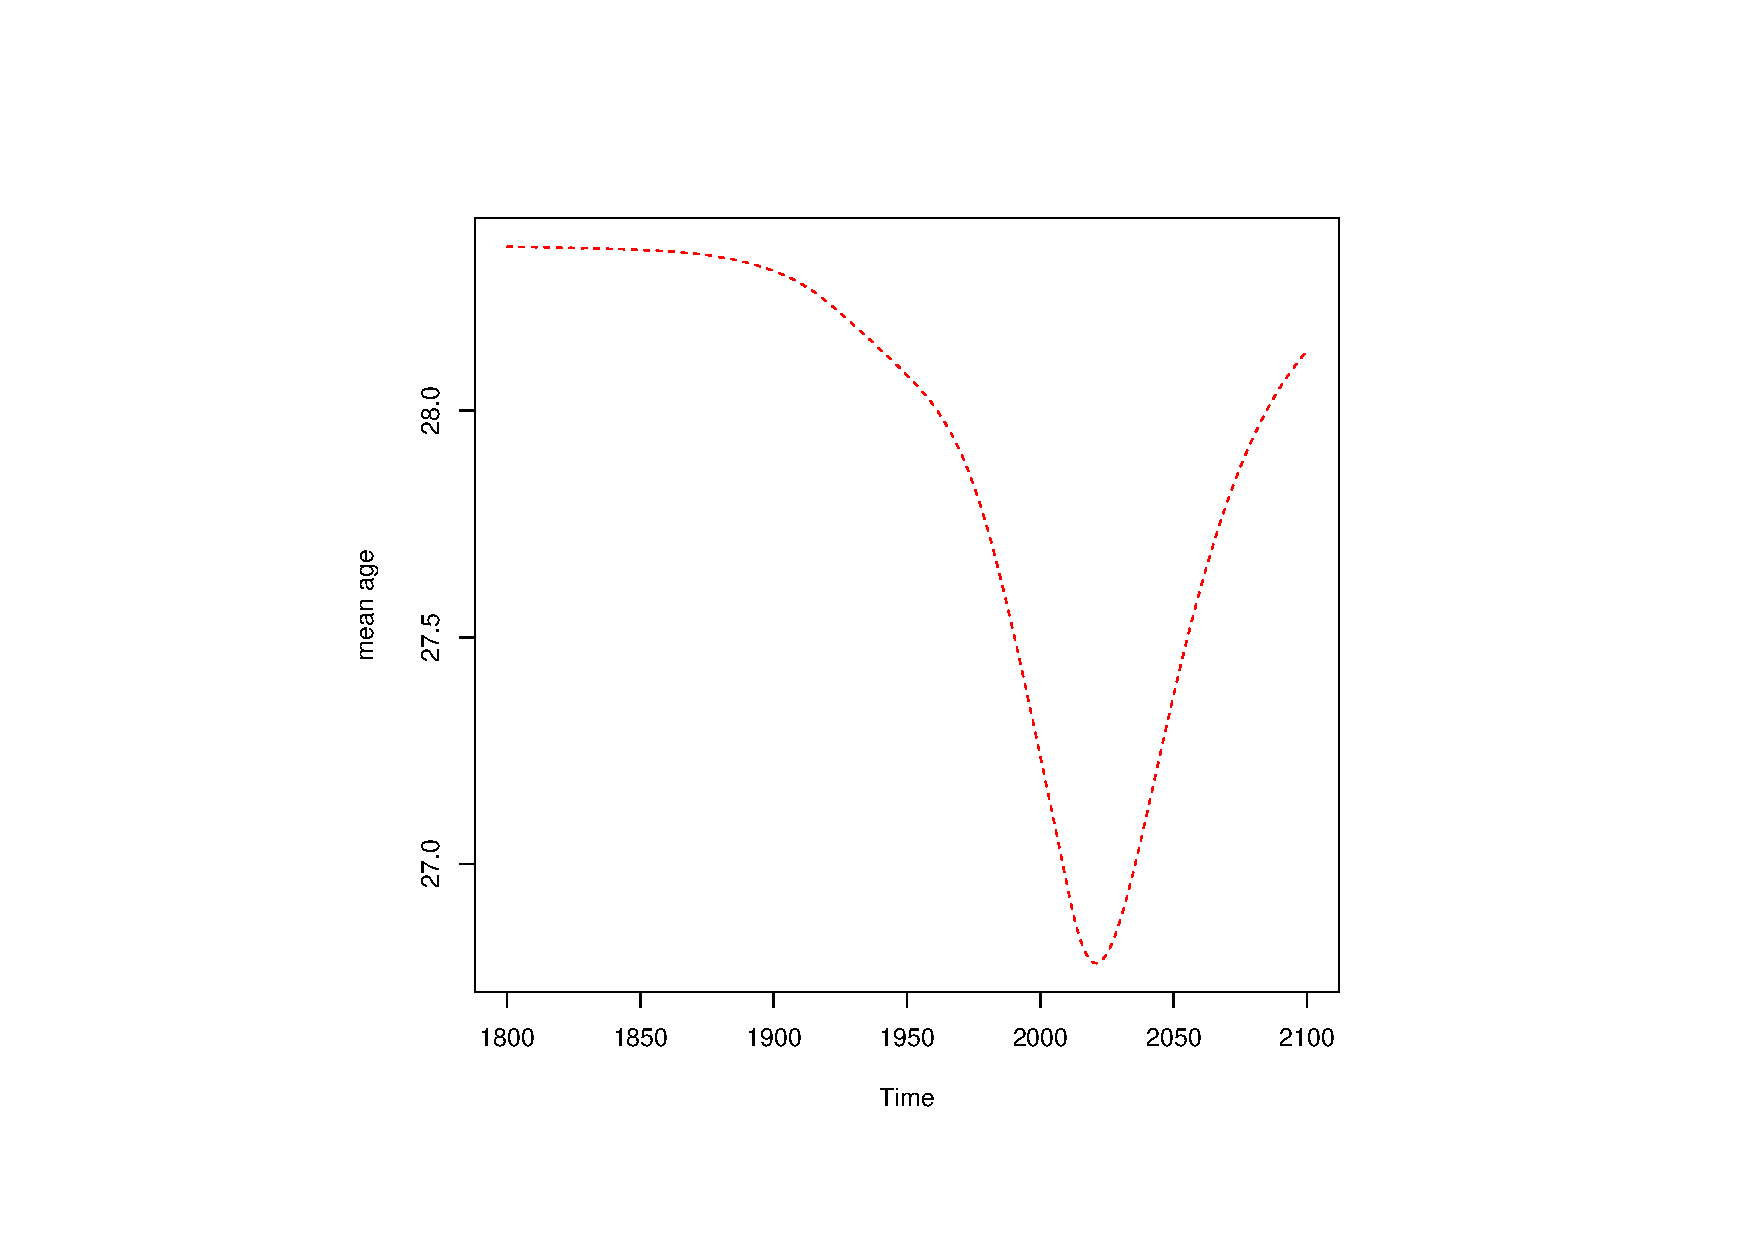
\includegraphics[width=0.9\textwidth]{NonlinearAtmosphericModelMeanAge.pdf}
%\end{frame}
%
%%%%%%%%%%%%%%%%%%%%%%%%%%%%%%%%%%%%%%%%%%%%%%%%%%%%%%%%%%%%%%%%%%%%%%%%%%%%%%%%%%%%%%%%%%%%%%%%%%%%%%
%\begin{frame}
% [fragile]
%\frametitle{Conclusions and outlook}
%\begin{itemize}
%      \pause
%   \item The previously available methods for the computation of mean ages and mean transit times
%      may lead to confusing interpretations if applied to time invariant systems.
%      \pause
%   \item One more generally applicable set of definitions has been proposed.
%      \pause
%   \item A numerical method has been (partly) developed to obtain the desired values for 
%      nonlinear, coupled, time variant systems.
%      \pause
%   \item The method has to be applied to coupled open systems
%      \pause
%   \item Other definitions of mean age and transit times could be evaluated for suitability.
%\end{itemize}
%\end{frame}
%%%%%%%%%%%%%%%%%%%%%%%%%%%%%%%%%%%%%%%%%%%%%%%%%%%%%%%%%%%%%%%%%%%%%%%%%%%%%%%%%%%%%%%%%%%%%%%%%%%%%%
\begin{frame}
 [fragile]
\frametitle{Thank you for your attention}
   \includegraphics<1>[width=\textwidth]{Verwirrung2.jpg}
%   \\
%   If you cannot win through you should at least create confusion...
\end{frame}

\lyxframeend{}
\begin{frame}
\frametitle{bibliography}
	\bibliography{/home/mm/SoilR/Bibliography/TEE-clean.bib}
\end{frame}
\end{document}
